% 本文件是 SolusMan-LADR4e 的一部分。
%
% Copyright (C) 2024 Songbingzhi628
%
% SolusMan-LADR4e is free software: you can redistribute it and/or modify
% it under the terms of the GNU Affero General Public License as
% published by the Free Software Foundation, either version 3 of the
% License, or any later version.
%
% This program is distributed in the hope that it will be useful,
% but WITHOUT ANY WARRANTY; without even the implied warranty of
% MERCHANTABILITY or FITNESS FOR A PARTICULAR PURPOSE.  See the
% GNU Affero General Public License for more details.
%
% You should have received a copy of the GNU Affero General Public License
% along with this program.  If not, see <https://www.gnu.org/licenses/>.
% Email: 13012057210@163.com

\ChDecl{Ch4}{4}{}\orMode{\hLk{4O2}{2}\;\;\hLk{4O3}{3}\;\;\hLk{4O4}{4}\;\;\hLk{4O5}{5}\;\;\hLk{4O6}{6}\;\;\hLk{4O7}{7}\;\;\hLk{4O8}{8}\;\;\hLk{4O9}{9}\;\;\hLk{4O10}{10}\;\;\hLk{4O11}{11}\;\;|\;\;\hLk{4O4e2}{4E:\;\;2}\;\;\hLk{4O4e3}{3}\;\;\hLk{4O4e13}{13}}{[2]: (4E 2), (4E 3), 4, 5, 2; [3]: 3, 6, 7, 9; [4]: 8, 11; [5]: 10, (4E 13).}

\vspace{3pt}

\ProblemBnoor[]{\Tips \,\,\,}[]{
	\TextB{\tgsl\large\envFontDefault Suppose $p\in\PoF{},\deg p\leqslant m$ and $p$ has at least $\Par{m+1}$ distinct zeros.}
	\Blind{\Tips \,\,\,} \TextB{\tgsl\large\envFontDefault Then by the contrapositive of [4.12], 又 $\deg p=m,$ we conclude that $m<0.$ Hence $p=0.$}
}\TextB{}
\Or We show that if $p$ has at least $m$ distinct zeros, then either $p=0$ or $\deg p\geqslant m.$\TextB{}
If $p=0$ then we are done. If not, then suppose $p$ has exactly $n$ distinct zeros $\lambda_1,\dots,\lambda_n.$\TextB{}
Because $\exists\,!\,\alpha_i\geqslant 1,q\in\PoF{},$ and $q\neq 0,$ such that $p\Par{z}=\Sbra{\Par{z-\lambda_1}{^{\alpha_1}}\cdots\Par{z-\lambda_n}{^{\alpha_n}}}q\Par{z}.$\PfEnd\vspace{2pt}

\ProblemBnoor[]{\Comment\,\,\,}[]{
	\TextB{\large\envFontDefault\NOTICE that by [4.17], some term of the poly factorization might not be in the form $\Par{x-\lambda_k}{^{\alpha_k}}.$\vspace{-6pt}}
}\SepLine

\BulletPointX\NoteFor{[4.7]} {\tgsl the uniqness of coeffs of polys} \hfill[{\tgsc Another proof}]\TextB{\vspace{2pt}}
If a poly had two different sets of coeffs, then
subtracting the two representations\TextB{}
would give a poly with some nonzero coeffs but infinitely many zeros. By \TIPS.\PfEnd\vspace{-3pt}
\SepLine

\BulletPointX\NoteFor{[4.8]} {\tgsl division algorithm for polys} \hfill[{\tgsc Another proof}]\TextB{\vspace{4pt}}
Suppose $\deg p\geqslant \deg s$. Then $\XPar{\underbrace{1, z,\dots, z^{\deg s-1}}_{\text{of\,length}\,\deg s},\underbrace{s,zs,\cdots,z^{\deg p-\deg s}s}_{\text{of\,length}\,\Par{\deg p-\deg s+1}}}$ is a basis of $\PoF{\deg p}.$\TextB{}
Because $q\in\PoF{},\exists\,!\,a_i,b_j\in\Fbb,$\TextB{}
$q=a_0+a_1 z+\dots+a_{\deg s-1}z^{\deg s-1}+ b_0 s+b_1 zs +\dots+ b_{\deg p-\deg s}z^{\deg p-\deg s}s$\TextB{}
$=\underbrace{a_0+a_1 z+\dots+a_{\deg s-1}z^{\deg s-1}}_{r}+s\underbrace{\XPar{b_0+b_1 z +\dots+ b_{\deg p-\deg s}z^{\deg p-\deg s}}}_{q}.$ Note that $r,q$ are unique.\PfEnd[-16pt]
\SepLine

\BulletPointX\NoteFor{[4.11]}\;\;{\tgsl each zero of a poly corresponds to a degree-one factor;}\hfill[{\tgsc Another proof}]\TextB{\vspace{2pt}}
First suppose $p\Par{\lambda}=0.$ Write $p\Par{z}=a_0+a_1 z+\dots+a_m z^m,\exists\,!\,a_0,a_1,\dots,a_m\in\Fbb$ for all $z\in\Fbb.$\vspace{2pt}\TextB{}
Then $p\Par{z}=p\Par{z}-p\Par{\lambda}=a_1\Par{z-\lambda}+\dots+a_m\Par{z^m-\lambda^m}$ for all $z\in\Fbb.$\vspace{2pt}\TextB{}
Hence $\forall k\in\Bra{1,\dots,m},z^k-\lambda^k=\Par{z-\lambda}\Par{ z^{k-1}\lambda^0+ z^{k-2}\lambda^1+\dots+z^{k-\Par{j+1}}\lambda^j+\dots+z\lambda^{k-2}+z^0\lambda^{k-1}}.$\vspace{4pt}\TextB{}
Thus $p\Par{z}=\sum_{j=1}^m a_j \Par{z-\lambda}\sum_{i=1}^k \lambda^{i-1}z^{k-i}=\Par{z-\lambda}\sum_{j=1}^m a_j\sum_{i=1}^k \lambda^{i-1}z^{k-i}=\Par{z-\lambda}q\Par{z}.$\PfEnd
\SepLine

\BulletPointX\NoteFor{[4.13]}\;\;{\tgsl Every nonconst poly with complex coefficients has a zero in $\Cbb$.} \vspace{2pt}\hfill[{\tgsc Another proof}]\TextB{}
For any $w\in\Cbb,k\in\Nbp,$ by polar coordinates, $\exists\,r\geqslant 0,\theta\in\Rbb,r\Par{\cos\theta + \i \sin\theta} = w$.\vspace{2pt}\TextB{}
By De Moivre' theorem, $w^k=\Sbra{r\Par{\cos\theta +\i\sin \theta}}{^k}=r^k\Par{\cos k\theta + \i \sin k\theta}$.\vspace{2pt}\TextB{}
Hence $\BigPar{r^{1/k}\Par{\cos\frac{\theta}{k} +\i\sin\frac{\theta}{k}}}{^k}=w$. Thus every complex number has a {\tgsl $k^{th}$ root}.\vspace{6pt}\TextB{}
Suppose a nonconst $p\in\PoC{}$ with highest-order nonzero term $c_m z_m.$\vspace{3pt}\TextB{}
Then $\aMid{p\Par{z}}\rightarrow\infty$ as $\aMid{z}\rightarrow\infty$ \XPar{ because $\Frac{\aMid{p\Par{z}}}{\aMid{z_m}}\rightarrow\aMid{c_m}$ as $\aMid{z}\rightarrow\infty$ }.\vspace{3pt}\TextB{}
\vspace{3pt}Thus the continuous function $z\rightarrow\aMid{p\Par{z}}$ has a global minimum at some point $\zeta\in\Cbb.$\TextB{}
\vspace{3pt}To show that $p\Par{\zeta} = 0$, assume $p\Par{\zeta}\neq 0$. Define $q\in\PoC{}$ by $q\Par{z}=\Frac{p\Par{z+\zeta}}{p\Par{\zeta}}.$\TextB{}
\vspace{3pt}The function $z\rightarrow\aMid{q\Par{z}}$ has a global minimum value of $1$ at $z = 0$.\TextB{}
\vspace{3pt}Write $q\Par{z} = 1 + a_k z^k + \dots + a_m z^m$, where $k\in\Nbp$ is the smallest such that $a_k\neq 0$.\TextB{}
\vspace{3pt}Let $\beta\in\Cbb$ be such that $\beta^k=-\Frac{1}{a_k}$.\TextB{}
\vspace{4pt}There is a const $c > 1$ so that if
$t\in \Par{0, 1}$, then $\aMid{q\Par{t\beta}}\leqslant\aMid{1 + a_k t^k\beta^k}+t^{k+1}c = 1 - t^k \Par{1 - tc}$.\TextB{}
Now letting $t=1/\Par{2c}$, we get $\aMid{q\Par{t\beta}}<1$. Contradicts. Hence $p\Par{\zeta} = 0$, as desired.\PfEnd
\SepLine\pagebreak

\ProblemBnoor{\hypertarget{4O4e2}{4E 4.2}}{
	\TextB{Prove that if $w,z\in\Cbb,$ then $\aXMid{\aMid{w}-\aMid{z}}\leqslant\aMid{w-z}.$}
}\par\quad
\vspace{-6pt}\AlignEq{}{
	\aMid{w-z}{^2}&=\Par{w-z}\Par{\overline{w}-\overline{z}}\hspace{380pt}\\
	&=\aMid{w}{^2}+\aMid{z}{^2}-\Par{w\overline{z}+\overline{w}z}\\
	&=\aMid{w}{^2}+\aMid{z}{^2}-\BigPar{\overline{\overline{w}z}+\overline{w}z}\\
	&=\aMid{w}{^2}+\aMid{z}{^2}-2Re\Par{\overline{w}z}\\
	&\geqslant\aMid{w}{^2}+\aMid{z}{^2}-2\aMid{\overline{w}z}\\
	&=\aMid{w}{^2}+\aMid{z}{^2}-2\aMid{w}\aMid{z}=\aXMid{\aMid{w}-\aMid{z}}{^2}.}\par
\vspace{-130pt}\hspace{200pt}$\hMath{l}{\left|}{\right.}{$\;\Or \!\!$\MathRightBrace{l}{
	\aMid{w}=\aMid{w-z+z}\leqslant\aMid{w-z}+\aMid{z}\Rightarrow \aMid{w}-\aMid{z}\leqslant\aMid{w-z}\\
	\aMid{z}=\aMid{z-w+w}\leqslant\aMid{z-w}+\aMid{w}\Rightarrow \aMid{z}-\aMid{w}\leqslant\aMid{w-z}}\\
	\;\\\;\text{\tgsl\normalsize Geometric interpretation: The length of each side of a triangle}\\
	\;\text{\tgsl\normalsize is greater than or equal to the difference of the lengths of the two other sides.}\\\;}$\PfEnd[7pt]\vspace{-2pt}
\SepLine

\ProblemBnoor{\hypertarget{4O4e3}{4E 4.3}}{
	\TextB{Suppose $\Fbb=\Cbb,\varphi\in V\apostrophe.$ Define $σ:V\rightarrow\Rbb$ by $\sigma\Par{v} = \mathfrak{Re}\,\varphi\Par{v}$ for each $v\in V.$\vspace{4pt}}
	\TextB{Show that $\varphi\Par{v}=\sigma\Par{v}-\i\sigma\Par{\i v}$ for all $v\in V.$\vspace{2pt}}
}Notice that \,$\varphi\Par{v}=\mathfrak{Re}\,\varphi\Par{v}+\i\,\mathfrak{Im}\,\varphi\Par{v}=\sigma\Par{v}+\i\,\mathfrak{Im}\,\varphi\Par{v}.$\par
\Blind{\Solution} 又 $\mathfrak{Re}\,\varphi\Par{\i\, v}=\mathfrak{Re}\BigPar{\i\,\varphi\Par{v}}=-\mathfrak{Im}\,\varphi\Par{v}=\sigma\Par{\i\,v}.$ Hence $\varphi\Par{v}=\sigma\Par{v}-\i\,\sigma\Par{\i\,v}.$\PfEnd
\SepLine

\ProblemN{\hypertarget{4O4}{4}}{
	\TextN{Suppose $m,n\in\Nbp$ with $m\leqslant n,\;\lambda_1,\dots,\lambda_m\in\Fbb.$}
	\TextN{Prove that $\exists\,p\in\PoF{},\deg p = n,$ the zeros of $\,p\,$ are $\lambda_1,\dots,\lambda_m.$\vspace{3pt}}
}Let $p\Par{z}=\Par{z-\lambda_1}^{{\envFontSmall[\scriptsize]n-\Par{m-1}}}\Par{z-\lambda_2}\cdots\Par{z-\lambda_m}.$\PfEnd
\SepLine

\ProblemN{\hypertarget{4O5}{5}}{
	\TextN{Suppose $m\in\Nbb,$ and $z_1,\dots,z_{m+1}$ are distinct in $\Fbb,$ and $w_1,\dots,w_{m+1}\in\Fbb.$}
	\TextN{Prove that $\exists\,!\,p\in\PoF{m},p\Par{z_k}=w_k$ for each $k\in\Bra{1,\dots, m+1}.$}
}\par\quad
Define $T:\PoF{m}\rightarrow\Fbb^{m+1}$ by $Tq=\BigPar{q\Par{z_1},\dots,q\Par{z_m},q\Par{z_{m+1}}}.$ Moreover, $T$ is linear.\vspace{4pt}\par\quad
We now show that $T$ is surj, so that such $p$ exists;\; and that $T$ is inje, so that such $p$ is unique.\vspace{1pt}\par\quad
Inje: $Tq=0\Longleftrightarrow q\Par{z_1}=\dots=q\Par{z_m}=q\Par{z_{m+1}}=0\Longleftrightarrow q=0,$ by \TIPS.\vspace{1pt}\par\quad
Surj: $\dim\range T=\dim\PoF{m}-\dim\null T=m+1=\dim\Fbb^{m+1}$ 又$\range T\subseteq\Fbb^{m+1}\Rightarrow T$ is surj.\PfEnd\vspace{8pt}\quad
\Or Let $p_1=1,\;p_k\Par{z}=\prod_{i=1}^{k-1}\Par{z-z_i}=\Par{z-z_1}\cdots\Par{z-z_{k-1}}$ for each $k\in\Bra{2,\dots,m+1}.$\vspace{2pt}\par\quad
By (2.C.10), $B_p=\Par{p_1,\dots,p_{m+1}}$ is a basis of $\PoF{m}.$ Let $B_e=\Par{e_1,\dots,e_{m+1}}$ be the std basis of $\Fbb^{m+1}.$\vspace{4pt}\par\quad
\NOTICE that $Tp_1=\Par{1,\dots,1},\;Tp_k=\XPar{\prod_{i=1}^{k-1}\Par{z_1-z_i},\dots,\underbrace{\prod_{i=1}^{k-1}\Par{z_j-z_i}}_{\envFontSmall[\scriptsize]j^{th}\text{ entry}},\dots,\prod_{i=1}^{k-1}\Par{z_{m+1}-z_i}}.$\vspace{2pt}\par\quad
And that $\prod_{i=1}^{k-1}\Par{z_j-z_i}=0\Longleftrightarrow j\leqslant k-1,$ because $z_1,\dots,z_{m+1}$ are distinct.\vspace{4pt}\par\quad
Thus $\Mt[\BigPar]{T,B_p,B_e}=\,${\normalsize$\begin{pmatrix}
	1 & 0 & 0 & \cdots & 0\\
	1 & A_{2,2} & 0 & \cdots & 0\\
	1 & A_{3,2} & A_{3,3} & \cdots & 0\\
	\vdots & \vdots & \vdots & \ddots & \vdots\\
	1 & A_{m+1,2} & A_{m+1,3} & \cdots & A_{m+1,m+1}
\end{pmatrix}$}.\vspace{6pt}\par\quad
Where $A_{j,k}=\prod_{i=1}^{k-1}\Par{z_j-z_i}\neq 0$ for all $j> k-1\geqslant 1.$ The rows of $\Mt{T}$ is linely inde.\vspace{4pt}\par\quad
By (4E 3.C.17) 又 $\dim\PoF{m}=\dim\Fbb^{m+1};\;$ \OR By (3.F.32); $T$ is inv.\PfEnd
\SepLine

\ProblemN{\hypertarget{4O2}{2}}{
	\TextN{Suppose $m\in\Nbp$. Is the set $U=\zeroSubs\cup\Bra{p\in\PoF{}:\deg p = m}$ a subsp of $\PoF{}$?}
}$x^m,x^m+x^{m-1}\in U$ \,\,but\,\, $\Deg\Sbra{\Par{x^m+x^{m-1}}-\Par{x^m}}\neq m\Rightarrow \Par{x^m+x^{m-1}}-\Par{x^m}\not\in U.$\PfEnd
\SepLine

\ProblemN{\hypertarget{4O3}{3}}{
	\TextN{Suppose $m\in\Nbp$. Is the set $U=\zeroSubs\cup\Bra{p\in\PoF{}:2\;\mmid\,\deg p}$ a subsp of $\PoF{}$?}
}$x^2,x^2+x\in U$ \,\,but\,\, $\Deg\Sbra{\Par{x^2+x}-\Par{x^2}}$ is odd and hence $\Par{x^2+x}-\Par{x^2}\not\in U.$\PfEnd
\SepLine

\ProblemN{\hypertarget{4O6}{6}}{
	\TextN{Suppose nonzero $p\in\PoF{m}$ has degree $m.$ Prove that}
	\TextN{[P] $p$ has $m$ distinct zeros $\Longleftrightarrow p$ and its derivative $p\apostrophe$ have no zeros in common [Q].}
}\par\quad
(a) Suppose $p$ has $m$ distinct zeros. And $\deg p=m.$ By [4.14], $\exists\,!\,c,\lambda_i\in\Rbb,p\Par{z}=c\Par{z-\lambda_1}\cdots\Par{z-\lambda_m}.$\par\vspace{2pt}\quad\Ha
If $m=0,$ then $p=c\neq 0\Rightarrow p$ has no zeros, and $p\apostrophe=0,$ we are done.\par\quad\Ha
If $m=1,$ then $p\Par{z}=c\Par{z-\lambda_1},$ and $p\apostrophe=c$ has no zeros, we are done.\par\vspace{2pt}\quad\Ha
For each $j\in\Bra{1,\dots,m}$, let $q_j\in\PoF{m-1}$ be such that ${p\Par{z}}={\Par{z-\lambda_j}}q_j\Rightarrow q_j\Par{\lambda_j}\neq 0.$\par\vspace{2pt}\quad\Ha
Now $p\apostrophe\Par{z}=\Par{z-\lambda_j}q_j\apostrophe\Par{z}+q_j\Par{z}\Rightarrow p\apostrophe\Par{\lambda_j}=q_j\Par{\lambda_j}\neq 0,$ as desired.\par\vspace{6pt}\quad\Ha
\Or To prove $[P]\Rightarrow[Q],$ we prove ${}^{\neg}[Q]\Rightarrow{}{^\neg}[P]$:\par\quad\Ha
Suppose $p\Par{z}=\Par{z-\lambda}q\Par{z},\;p\apostrophe\Par{z}=\Par{z-\lambda}r\Par{z}.$ 又 $p\apostrophe\Par{z}=\Par{z-\lambda}q\apostrophe\Par{z}+q\Par{z}.$\vspace{2pt}\par\quad\Ha
Now $p\apostrophe\Par{\lambda}=q\Par{\lambda}=0\Rightarrow q\Par{z}=\Par{z-\lambda}s\Par{z},p\Par{z}=\Par{z-\lambda}{^2}s\Par{z}.$\vspace{2pt}\par\quad\Ha
Hence $p$ has strictly less than $m$ distinct zeros.\par\vspace{6pt}\quad
(b) To prove $[Q]\Rightarrow[P]$, we prove ${}^{\neg}[P]\Rightarrow{}{^\neg}[Q]$:\par\quad\Hb
Because nonzero $p\in\PoF{m},$ we suppose $\lambda_1,\dots,\lambda_M$ are all the distinct zeros of $p,$ where $M<m.$\vspace{2pt}\par\quad\Hb
By Pigeon Hole Principle, $\exists\,\lambda_k$ such that $p\Par{z}=\Par{z-\lambda_k}{^{2}}q\Par{z}$ for some $q\in\PoF{}.$\vspace{3pt}\par\quad\Hb
Hence $p\apostrophe\Par{z}=2\Par{z-\lambda_k}q\Par{z}+\Par{z-\lambda_k}{^2}q\apostrophe\Par{z}\Rightarrow p\apostrophe\Par{\lambda_k}=0=p\Par{\lambda_k}.$\PfEnd
\SepLine

\ProblemN{\hypertarget{4O7}{7}}{
	\TextN{Prove that every $p\in\PoR{}$ of odd degree has a zero.}
}\par\quad
Using the notation and proof of [4.17]. $\deg p=2M+m$ is odd $\Rightarrow m$ is odd. Hence $\lambda_1$ exists.\PfEnd\vspace{6pt}\quad
\Or Using calculus only. Suppose $p\in\PoF{m},\deg p=m,m$ is odd.\par\quad
Let $p\Par{x}=a_0+a_1 x+\dots+a_m x^m.$ Then $a_m\neq 0.$ Denote $\aMid{a_m}{^{-1}}a_m$ by $\delta.$\par\vspace{3pt}\quad
Write $p\Par{x}=x^m\XPar{\Frac{a_0}{x^m}+\Frac{a_1}{x^{m-1}}+\dots+\Frac{a_{m-1}}{x}+a_m}.$\par\vspace{5pt}\quad
Thus $p\Par{x}$ is continuous, and $\lim\limits_{x\rightarrow -\infty}p\Par{x}=-\delta\infty\,;\quad\lim\limits_{x\rightarrow \infty}p\Par{x}=\delta\infty.$\par\quad
Hence we conclude that $p$ has at least one real zero.\PfEnd
\SepLine

\ProblemN{\hypertarget{4O9}{9}}{
	\TextN{Suppose $p\in\PoC{}$. Define $q:\Cbb\rightarrow\Cbb\,$ by $q\Par{z} = p\Par{z}\overline{p\Par{\overline z}}$. Prove that $q\in\PoR{}$.}
}\par\quad
\NOTICE that by [4.5], $\overline z{^n}=\overline{z^n}.$\par\quad
Suppose $q\Par{z}=a_n z^n+\dots+a_1 z+a_0\Rightarrow q\Par{\overline z}=a_n \overline z{^n}+\dots+a_1 \overline z+a_0\Rightarrow \overline{q\Par{\overline z}}=\overline{a_n}z^n+\dots+\overline{a_1}z+\overline{a_0}.$\vspace{8pt}\par\quad
Note that $q\Par{z}=p\Par{z}\overline{p\Par{\overline z}}=\overline{p\Par{\overline z}}p\Par{z}=\overline{p\Par{\overline z}\overline{\overline{p\Par{\overline z}}}}=\overline{q\Par{\overline z}}.$ Hence for each $a_k,\overline{a_k}=a_k\Rightarrow a_k\in\Rbb.$\PfEnd\vspace{14pt}\quad
\Or Suppose $p\Par{z}=a_m z^m+\dots+a_1z+a_0.$ Now $\overline{p\Par{\overline z}}=\overline{a_m} z^m+\dots+\overline{a_1}z+\overline{a_0}.$\vspace{4pt}\par\quad
\NOTICE that $q\Par{z}=p\Par{z}\overline{p\Par{\overline z}}=\sum_{k=0}^2m\XPar{\sum_{i+j=k}a_i\overline{a_j}}z^k.$\vspace{4pt}\par\quad
\NOTICE that by [4.5], $z-\overline z=2\Par{\mathfrak{Im}\,z}\Rightarrow z=\overline z+2\Par{\mathfrak{Im}\,z}.$ So that $z=\overline z\Longleftrightarrow\mathfrak{Im}\,z=0\Longleftrightarrow z\in\Rbb.$\vspace{4pt}\par\quad
Now for each $k\in\Bra{0,\dots,2m},\overline{\sum_{i+j=k}a_i\overline{a_j}}=\sum_{i+j=k}\overline{a_i\overline{a_j}}=\sum_{i+j=k}{a_j}\overline{a_i}=\sum_{i+j=k}a_i\overline{a_j}\in\Rbb.$\PfEnd
\SepLine\pagebreak

\ProblemN{\hypertarget{4O8}{8}}{
	\TextN{For $p\in\PoR{}$, define $Tp:\Rbb\rightarrow\Rbb\,$ by $\Par{Tp}\Par{x}=\,${\large\envFontDefault$\MathLeftBrace{l}{
		\Frac{p\Par{x}-p\Par{3}}{x-3}\;$ if $x\neq 3,\\[4pt]
		p\apostrophe\Par{3}$\hfill if $x=3.
	}$}\vspace{6pt}}
	\TextN{Show that {\tgnr(a)} $Tp\in\PoR{}$ for all $p\in\PoR{}$ and that {\tgnr(b)} $T:\PoR{}\rightarrow\PoR{}$ is linear.}
}\vspace{2pt}\par\quad
(a) For $x\neq 3,T\Par{x^n}=\Frac{x^n-3^n}{x-3}=\sum_{i=1}^n 3^{i-1}x^{n-i}.$ For $x=3,T\Par{x^n}=3^{n-1}\cdot n.$\vspace{6pt}\par\quad\Ha
Note that if $x=3,$ then $\sum_{i=1}^n 3^{i-1}x^{n-i}=\sum_{i=1}^n 3^{n-1}=3^{n-1}\cdot n.$\vspace{2pt}\par\quad\Ha
Hence $T\Par{x^n}=\sum_{i=1}^n 3^{i-1}x^{n-i}\Rightarrow T\Par{x^n}\in\PoR{}.$\par\vspace{6pt}\quad
(b) Now we show that $T$ is linear: $\forall p,q\in\PoR{},\lambda\in\Rbb,$\vspace{6pt}\par\quad\Hb
$T\Par{p+\lambda q}\Par{x}=\,${\normalsize\envFontSmall$\hMath{l}{\left\{}{\right|}{
		\Frac{\Par{p+\lambda q}\Par{x}-\Par{p+\lambda q}\Par{3}}{x-3},\;$ if $x\neq 3,\\
		\Par{p+\lambda q}\apostrophe\Par{3},$ \hfill if $x=3\Blind{.}
	}$}$\;=\Sbra{T\Par{p}+\lambda T\Par{q}}\Par{x}$ for all $x\in\Rbb.$\PfEnd\vspace{16pt}\quad
\Or (a) Note that $\exists\,!\,q\in\PoR{},p\Par{x}-p\Par{3}=\Par{x-3}q\Par{z}\Rightarrow q\Par{x}=\Frac{p\Par{x}-p\Par{3}}{x-3}.$\vspace{4pt}\par\quad\Ha
\Blind{\Or} $p\apostrophe\Par{x}=\BigPar{p\Par{x}-p\Par{3}}\apostrophe=\BigPar{\Par{x-3}q\Par{x}}\apostrophe=q\Par{x}+\Par{x-3}q\apostrophe\Par{x}.$\vspace{2pt}\par\quad\Ha
\Blind{\Or} Hence $p\apostrophe\Par{3}=q\Par{3}.$ Now $Tp=q\in\PoR{}.$\vspace{6pt}\par\quad
\Blind{\Or} (b) $\forall p_1,p_2\in\PoR{},\lambda\in\Rbb,\exists\,!\,q_1,q_2\in\PoR{},$\vspace{2pt}\par\quad\Hb
\Blind{\Or} $p_1\Par{x}-p_1\Par{3}=\Par{x-3} q_1\Par{x}$ and $p_2\Par{x}-p_2\Par{3}=\Par{x-3} q_2\Par{x}.$\vspace{2pt}\par\quad\Hb
\Blind{\Or} By (a), $Tp_1=q_1,Tp_2=q_2.$ Note that $\Par{p_1+\lambda p_2}\Par{x}-\Par{p_1+\lambda p_2}\Par{3}=\Par{x-3}\Par{q_1+\lambda q_2}\Par{x}.$\vspace{2pt}\par\quad\Hb
\Blind{\Or} Hence by the uniqnes of $q_1+\lambda q_2$ for $p_1+\lambda p_2,$ we must have $T\Par{p_1+\lambda p_2}=q_1+\lambda q_2.$\PfEnd
\SepLine

\ProblemN{\hypertarget{4O11}{11}}{
	\TextNL{Suppose $p\in\PoF{}$ with $p\neq 0$. Let $U=\Bra{pq:q\in\PoF{}}$.}
	(a) \TextNL{Show that $\dim\PoF{}\mySlash U = \deg p$.}
	(b) \TextNL{Find a basis of $\PoF{}\mySlash U$.}
}\NOTICE that $pq\neq p\circ q,$ see (4E 3.A.10).\par\quad
$U$ is a subsp of $\PoF{}$ because $\forall s_1,s_2\in\PoF{},\lambda\in\Fbb,ps_1+\lambda ps_2=p\Par{s_1+\lambda s_2}\in U.$\par\vspace{3pt}\quad
If $\deg p=0,$ then $U=\PoF{},\PoF{}\mySlash U=\Bra{0},$ with the unique basis $\Par{}.$ Suppose $\deg p\geqslant 1.$\par\vspace{6pt}\quad
(a) By [4.8], $\forall s\in\PoF{},\exists\,!\,r\in\PoF{\deg p-1},q\in\PoF{}\,\Sbra{\,\exists\,!\,pq\in U\,},s=\Par{p}q+\Par{r}.$\vspace{2.5pt}\par\quad\Ha
Thus $\PoF{}=U\oplus\PoF{\deg p-1}.$ By the \NOTEFOR\;[3.91] in (3.E), $\PoF{}\mySlash U$ and $\PoF{\deg p-1}$ are iso.\par\vspace{4.5pt}\quad\Ha
\Or Define $R:\PoF{}\rightarrow\PoF{\deg p-1}$ by $R\Par{s}=r$ for all $s\in\PoF.$ We show that $R$ is linear.\vspace{2pt}\par\quad\Ha
$\forall s_1,s_2\in\PoF{},\lambda\in\Fbb,\exists\,!\,r_1,r_2\in\PoF{\deg p-1},q_1,q_2\in\PoF{},s_1=\Par{p}q_1+\Par{r_1};\;s_2=\Par{p}q_2+\Par{r_2}.$\vspace{2pt}\par\quad\Ha
又 $\exists\,!\,r\in\PoF{\deg p-1},q\in\PoF{},\Par{s_1+\lambda s_2}=\Par{p}q+\Par{r}=\Par{p}\Par{q_1+\lambda q_2}+\Par{r_1+\lambda r_2}.$\vspace{2pt}\par\quad\Ha
Note that $r_1,r_2\in\PoF{\deg p-1}\Rightarrow r_1+\lambda r_2\in\PoF{\deg p-1}.$\vspace{2pt}\par\quad\Ha
\OR Note that $\Deg\Par{r_1+\lambda r_2}\leqslant\max\!\Bra{\deg r_1,\Deg\Par{\lambda r_2}}\leqslant\max\!\Bra{\deg r_1,\deg r_2}<\deg p.$\vspace{2pt}\par\quad\Hb
By the uniqnes part of [4.8], $s=s_1+\lambda s_2;\;r=r_1+\lambda r_2.$
Thus $R\Par{s_1+\lambda s_2}=R\Par{s_1}+\lambda R\Par{s_2}.$\vspace{6pt}\par\quad\Ha
Because $Rs=0\Longleftrightarrow s=pq,\exists\,!\,q\in\PoF{}\Longleftrightarrow s\in U.$ And $\forall r\in\PoF{\deg p-1},Rr=r.$\vspace{2pt}\par\quad\Ha
Now $\null R=U,\;\range R=\PoF{\deg p-1}.$\vspace{3pt}\par\quad\Ha
Hence $\tilde{R}:\PoF{}\mySlash U\rightarrow\PoF{\deg p-1}$ is defined by $\tilde{R}\Par{s+U}=Rs.$ By [3.91(d)], $\tilde{R}$ is an iso.\par\vspace{6pt}\quad
(b) For each $k\in\Bra{0,1,\dots,\deg p-1},\tilde{R}\Par{z^k+U}=R\Par{z^k}=z^k\Rightarrow \tilde{R}{^{-1}}\Par{z^k}=z^k+U.$\par\quad\Hb
Thus $\Par{1+U,z+U,\dots,z^{\deg p-1}+U}$ can be a basis of $\PoF{}\mySlash U.$\PfEnd
\SepLine

\ProblemN{\hypertarget{4O10}{10}}{
	\TextNL{Suppose $m\in\Nbb,p\in\PoC{m}$ is such that $p\Par{x_k}\in\Rbb$ for each of distinct $x_0,x_1,\dots,x_m\in\Rbb.$}
	\TextNL{Prove that $p\in\PoR{}$.}
}\par\quad
By \TIPS and Problem (5), $\exists\,!\,q\in\PoR{m}$ such that $q\Par{x_k}=p\Par{x_k}.$ Hence $p=q.$\PfEnd\vspace{6pt}\quad
\Or Using the Lagrange Interpolating Polynomial.\par\vspace{6pt}\quad
Define $q\Par{x}=\displaystyle\sum\limits_{j=0}^m\frac{\Par{x-x_0}\Par{x-x_1}\cdots\Par{x-x_{j-1}}\Par{x-x_{j+1}}\cdots\Par{x-x_m}}{\Par{x_j-x_0}\Par{x_j-x_1}\cdots\Par{x_j-x_{j-1}}\Par{x_j-x_{j+1}}\cdots\Par{x_j-x_m}}p\Par{x_j}.$\par\vspace{4pt}\quad
又 Each $x_j,\,p\Par{x_j}\in\Rbb\Rightarrow q\in\PoR{m}.$ Notice that $q\Par{x_k}=1\cdot p\Par{x_k}\Rightarrow \Par{q-p}\Par{x_k}=0$ for each $x_k.$\par\quad
Then $\Par{q-p}$ has $\Par{m+1}$ zeros, while $\Par{q-p}\in\PoC{m}$. By \TIPS, $q-p=0\Rightarrow p=q\in\PoR{}.$\PfEnd
\SepLine

\ProblemBnoor{\hypertarget{4O4e13}{4E 4 13}}{
	\TextB{Suppose nonconst $p,q\in\PoC{}$ have no zeros in common. Let $m = \deg p$, $n = \deg q$.\vspace{3pt}}
	\TextB{Define $T:\PoC{n-1}\times\PoC{m-1}\rightarrow\PoC{m+n-1}$ by $T\Par{r, s} = rp + sq.$ Prove that $T$ is an iso.\vspace{3pt}}
	\Corollary \,\,\,\TextB{$\exists\,!\,r\in\PoC{n-1},s\in\PoC{m-1}$ such that $rp + sq = 1.$}
}\par\quad
$T$ is linear because $\forall\,r_1,r_2\in\PoC{n-1},s_1,s_2\in\PoC{m-1},\lambda\in\Fbb,$\par\quad
$T\BigPar{\Par{r_1,s_1}+\lambda\Par{r_2,s_2}}=T\Par{r_1+\lambda r_2,s_1+\lambda s_2}=\Par{r_1+\lambda r_2}p+\Par{s_1+\lambda s_2}q=T\Par{r_1,s_1}+\lambda T\Par{r_2,s_2}.$\par\vspace{6pt}\quad
Let $\lambda_1,\dots,\lambda_M$ and $\mu_1,\dots,\mu_N$ be the distinct zeros of $p$ and $q$ respectively. \NOTICE that $M\leqslant m,N\leqslant n.$\vspace{2pt}\par\quad
Note that the contrapositive of [4.13], $M=0\Longleftrightarrow m=0\Rightarrow s=0\Longleftrightarrow r=0 \Leftarrow n=0\Longleftrightarrow N=0.$\vspace{2pt}\par\quad
Now suppose $M,N\geqslant 1.$ We show that $s=0.$ Showing $r=0$ is almost the same.\vspace{2pt}\par\quad
Write $p\Par{z}=a\Par{z-\lambda_1}{^{\alpha_1}}\cdots\Par{z-\lambda_M}{^{\alpha_M}}.$ \BigPar{ $\exists\,!\,\alpha_j\geqslant 1,a\in\Fbb.$ } Let $\max\!\Bra{\alpha_1,\dots,\alpha_M}=A.$\vspace{2pt}\par\quad
For each $D\in\Bra{0,1,\dots,A-1},$ let $I_{D,\alpha}=\Bra{{\gamma_{D,1}},\dots,{\gamma_{D,J}}}$ be such that each $\alpha_{\gamma_{D,j}}\geqslant D+1.$\vspace{2pt}\par\quad
Note that $I_{A-1,\alpha}\subseteq \cdots\subseteq I_{0,\alpha}=\Bra{1,\dots,M}.$ Because $rp+sq=0\Rightarrow\Par{rp+sq}{^{\SmallPar{k}}}=0$ for all $k\in\Nbp.$\vspace{2pt}\par\quad
We use induction by $D$ to show that $s{^{\SmallPar{D}}}\Par{\lambda_{\gamma_{D,j}}}=0$ for each $D\in\Bra{0,\dots,A-1}.$\vspace{2pt}\par\quad
\NOTICE that $p{^{\SmallPar{D}}}\Par{\lambda_\gamma}=0$ for each $D\in\Bra{0,\dots,A-1}$ and each $\lambda_\gamma\in I_{D,\alpha}.$\hfill{$\Par{\Delta}$}\vspace{2pt}\par\quad
(i) $D=0.$ $\Par{rp+sq}\Par{\lambda_{\gamma_{0,j}}}=\Par{sq}\Par{\lambda_{\gamma_{0,j}}}=s\Par{\lambda_{\gamma_{0,j}}}=0.$\vspace{2pt}\par\quad\Hi
$D=1.$ $\Par{rp+sq}\apostrophe\Par{\lambda_{\gamma_{1,j}}}=\Par{r\apostrophe p+rp\apostrophe}\Par{\lambda_{\gamma_{1,j}}}+\Par{s\apostrophe q+sq\apostrophe}\Par{\lambda_{\gamma_{1,j}}}=\Par{s\apostrophe q}\Par{\lambda_{\gamma_{1,j}}}=s\apostrophe\Par{\lambda_{\gamma_{1,j}}}=0.$\vspace{4pt}\par\quad\Endi
(ii) $2\leqslant D\leqslant A-1.$ Assume that $\;s{^{\SmallPar{d}}}\Par{\lambda_{\gamma_{d,j}}}=0$ for each $d\in\Bra{1,\dots,D-1}$ and each $\lambda_{\gamma_{d,j}}\in I_{d,\alpha}.$\vspace{2pt}\par\quad\Hii
\XPar{ Because $\forall p,q\in\PoF{},k\in\Nbp,\Par{pq}{^{\SmallPar{k}}}=\mathC_{k}^k p{^{\SmallPar{k}}}q{^{\SmallPar{0}}}+\dots+\mathC_{k}^j p{^{\SmallPar{j}}}q{^{\SmallPar{k-j}}}+\dots+\mathC_{k}^0 p{^{\SmallPar{0}}}q{^{\SmallPar{k}}}.$ }\hfill{$\Par{\Delta}$}\vspace{4pt}\par\quad\Hii
Now $\Sbra{rp+sq}{^{\SmallPar{D}}}\Par{\lambda_{\gamma_{D,j}}}=\Sbra{\mathC_{D}^D r{^{\SmallPar{D}}}p{^{\SmallPar{0}}}+\dots+\mathC_{D}^d r{^{\SmallPar{d}}}p{^{\SmallPar{D-d}}}+\dots+\mathC_{D}^0 r{^{\SmallPar{0}}}p{^{\SmallPar{D}}}}\Par{\lambda_{\gamma_{D,j}}}$\vspace{4pt}\par\quad\Hii
\Blind{Now} $\Blind{\Sbra{rp+sq}{^{\SmallPar{D}}}\Par{\lambda_{\gamma_{D,j}}}=}+\Sbra{\mathC_{D}^D s{^{\SmallPar{D}}}q{^{\SmallPar{0}}}+\dots+\mathC_{D}^d s{^{\SmallPar{d}}}q{^{\SmallPar{D-d}}}+\dots+\mathC_{D}^0 s{^{\SmallPar{0}}}q{^{\SmallPar{D}}}}\Par{\lambda_{\gamma_{D,j}}}$\vspace{4pt}\par\quad\Hii
\Blind{Now} $\Blind{\Sbra{rp+sq}{^{\SmallPar{D}}}\Par{\lambda_{\gamma_{D,j}}}}=\Sbra{\mathC_{D}^D s{^{\SmallPar{D}}}q{^{\SmallPar{0}}}}\Par{\lambda_{\gamma_{D,j}}}.$\; Where each $\lambda_{\gamma_{D,j}}\in I_{D,\alpha}\subseteq I_{D-1,\alpha}.$\vspace{4pt}\par\quad\Hii
Hence $s{^{\SmallPar{D}}}\Par{\lambda_{\gamma_{D,j}}}=0.$ The assumption holds for all $D\in\Bra{0,\dots,A-1}.$\vspace{6pt}\par\quad
\NOTICE that $\forall k=\Bra{0,\dots,A-2},s{^{\SmallPar{k}}}$ and $s{^{\SmallPar{k+1}}}$ have zeros $\Bra{\lambda_{\gamma_{k+1,1}},\dots,\lambda_{\gamma_{k+1,J}}}$ in common.\vspace{2pt}\par\quad
Now $\forall D\in\Bra{1,A-1},s=s{^{\SmallPar{0}}},\dots,s{^{\SmallPar{D}}}$ have zeros $\Bra{\lambda_{\gamma_{D,1}},\dots,\lambda_{\gamma_{D,J}}}$ in common.\vspace{2pt}\par\quad
Thus $\forall D\in\Bra{0,A-1},\;s\Par{z}$ is divisible by $\Par{z-\lambda_{\gamma_{D,1}}}{^{\alpha_{\gamma_{D,1}}}}\cdots\Par{z-\lambda_{\gamma_{D,J}}}{^{\alpha_{\gamma_{D,J}}}}.$\vspace{2pt}\par\quad
Hence we write $s\Par{z}=\XPar{\Par{z-\lambda_1}{^{\alpha_1}}\cdots\Par{z-\lambda_M}{^{\alpha_M}}}\,s_0\Par{z},$ while $\deg s\leqslant m-1<m=\alpha_1+\dots+\alpha_M.$\vspace{2pt}\par\quad
Thus by \TIPS, $s=0.$ Following the same pattern, we conclude that $r=0.$\vspace{2pt}\par\quad
Hence $T$ is inje. And $\Dim\BigPar{\PoC{n-1}\times\PoC{m-1}}=\dim\PoC{m+n-1}\Rightarrow T$ is surj. Thus $T$ is an iso.\PfEnd
\SepLine\pagebreak
\Comment\,\,\, We now prove the statement that marked by $\Par{\Delta}$ above.\vspace{6pt}\par
\ProblemN{L1:}{
	\TextB{Prove that $\forall p,q\in\PoF{},k\in\Nbp,\Par{pq}{^{\SmallPar{k}}}=\mathC_{k}^k p{^{\SmallPar{k}}}q{^{\SmallPar{0}}}+\dots+\mathC_{k}^j p{^{\SmallPar{j}}}q{^{\SmallPar{k-j}}}+\dots+\mathC_{k}^0 p{^{\SmallPar{0}}}q{^{\SmallPar{k}}}.$}
}\par\quad
We use induction by $k\in\Nbp.$\par\quad
(i) $k=1.$ $\Par{pq}{^{\SmallPar{1}}}=pq=C_{1}^1 p{^{\SmallPar{1}}}q{^{\SmallPar{0}}}+C_{1}^0 p{^{\SmallPar{0}}}q{^{\SmallPar{1}}}.$\par\quad\Endi
(ii) $k\geqslant 2.$ Assume that for $\Par{pq}{^{\SmallPar{k-1}}}=\mathC_{k-1}^{k-1} p{^{\SmallPar{k-1}}}q{^{\SmallPar{0}}}+\dots+\mathC_{k-1}^j p{^{\SmallPar{j}}}q{^{\SmallPar{k-1-j}}}+\dots+\mathC_{k-1}^0 p{^{\SmallPar{0}}}q{^{\SmallPar{k-1}}}.$\vspace{4pt}\par\quad\Hii
Now $\Par{pq}{^{\SmallPar{k}}}=\BigPar{\Par{pq}{^{\SmallPar{k-1}}}}\apostrophe=\XPar{\sum_{j=0}^{k-1}\mathC_{k-1}^{j} p{^{\SmallPar{j}}}q{^{\SmallPar{k-j-1}}}}\apostrophe=\sum_{j=0}^{k-1}\XSbra{\mathC_{k-1}^{j} \XPar{p{^{\SmallPar{j+1}}}q{^{\SmallPar{k-j-1}}}+p{^{\SmallPar{j}}}q{^{\SmallPar{k-j}}}}}.$\vspace{4pt}\par\quad\Hii
\Blind{Now} $\Blind{\Par{pq}{^{\SmallPar{k}}}\!}=\XSbra{\mathC_{k-1}^{0}\XPar{ \uwave{p{^{\SmallPar{1}}}q{^{\SmallPar{k-1}}}}+\boxed{p{^{\SmallPar{0}}}q{^{\SmallPar{k}}}}}}+\XSbra{\mathC_{k-1}^1\XPar{p{^{\SmallPar{2}}}q{^{\SmallPar{k-2}}}+\uwave{p{^{\SmallPar{1}}}q{^{\SmallPar{k-1}}}}}}$\vspace{6pt}\par\quad\Hii
\Blind{Now} $\Blind{\Par{pq}{^{\SmallPar{k}}}=}+\dots+\XSbra{\mathC_{k-1}^{j-2}\XPar{ \uline{p{^{\SmallPar{j-1}}}q{^{\SmallPar{k-j+1}}}}+p{^{\SmallPar{j-2}}}q{^{\SmallPar{k-j+2}}}}}+\XSbra{\mathC_{k-1}^{j-1}\XPar{ \uuline{p{^{\SmallPar{j}}}q{^{\SmallPar{k-j}}}}+\uline{p{^{\SmallPar{j-1}}}q{^{\SmallPar{k-j+1}}}}}}$\vspace{4pt}\par\quad\Hii
\Blind{Now} $\Blind{\Par{pq}{^{\SmallPar{k}}}=}+\XSbra{\mathC_{k-1}^{j}\XPar{ \uwave{p{^{\SmallPar{j+1}}}q{^{\SmallPar{k-j-1}}}}+\uuline{ p{^{\SmallPar{j}}}q{^{\SmallPar{k-j}}}}}}+\XSbra{\mathC_{k-1}^{j+1}\XPar{p{^{\SmallPar{j+2}}}q{^{\SmallPar{k-j-2}}}+\uwave{p{^{\SmallPar{j+1}}}q{^{\SmallPar{k-j-1}}}}}}$\vspace{4pt}\par\quad\Hii
\Blind{Now} $\Blind{\Par{pq}{^{\SmallPar{k}}}=}+\dots+\XSbra{\mathC_{k-1}^{k-2}\XPar{ \uline{p{^{\SmallPar{k-1}}}q{^{\SmallPar{1}}}}+p{^{\SmallPar{k-2}}}q{^{\SmallPar{2}}}}}+\XSbra{\mathC_{k-1}^{k-1}\XPar{ \boxed{p{^{\SmallPar{k}}}q{^{\SmallPar{0}}}}+\uline{p{^{\SmallPar{k-1}}}q{^{\SmallPar{1}}}}}}.$\vspace{4pt}\par\quad\Hii
Hence $\Par{pq}{^{\SmallPar{k}}}=\mathC_{k}^0{p{^{\SmallPar{0}}}q{^{\SmallPar{k}}}}+\dots+\XSbra{\mathC_{k-1}^{j}+\mathC_{k-1}^{j-1}}\BigPar{p{^{\SmallPar{j}}}q{^{\SmallPar{k-j}}}}+\dots+\mathC_{k}^{k}{p{^{\SmallPar{k}}}q{^{\SmallPar{0}}}}.$\PfEnd
\SepLine

\ProblemN{L2:}{
	\TextB{Suppose $p\Par{z}=\Par{z-\lambda}{^\alpha}q\Par{z}$ and $\alpha\in\Nbp.$ Prove that ${p{^{\SmallPar{\alpha-1}}}}\Par{\lambda}=0.$}
}\par\quad
Suppose $p\in\PoF{}.$ Write $p\Par{z}=\Par{z-\lambda}{^A}q\Par{z},$ where $A\in\Nbp,q\Par{\lambda}\neq 0.$\vspace{2pt}\par\quad
We use induction to show that for all $\alpha\in\Bra{1,\dots,A},{p{^{\SmallPar{\alpha-1}}}}\Par{\lambda}=0.$\vspace{2pt}\par\quad
(i) $\alpha=1.$ $p{^{\SmallPar{0}}}\Par{\lambda}=0.$\par\quad\Endi
(ii) $2\leqslant\alpha\leqslant A.$ Assume that $p{^{\SmallPar{a-2}}}\Par{\lambda}=0$ for all $a\in\Bra{1,\dots,\alpha}.$\par\quad\Hii
\NOTICE that $p\Par{z}=\Par{z-\lambda}{^{\alpha-1}}q_{\alpha-1}\Par{z}=\Par{z-\lambda}{^{\alpha}}q_{\alpha}\Par{z},$ where $q_{\alpha}\Par{z}=\Par{z-\lambda}q_{\alpha-1}\Par{z}.$\vspace{2pt}\par\quad\Hii
Because $p{^{\SmallPar{\alpha-1}}}\Par{z}=\XSbra{\mathC_{\alpha-1}^{\alpha-1}\Par{z-\lambda}{^{0}}q_{\alpha-1}\Par{z}+\dots+\mathC_{\alpha-1}^{k}\Par{z-\lambda}{^{\alpha-1-k}}q_{\alpha-1-k}\Par{z}$\vspace{2pt}\par\quad\Hii
\Blind{Because} $\Blind{p{^{\SmallPar{\alpha-1}}}\Par{z}=}+\dots+\mathC_{\alpha-1}^{0}\Par{z-\lambda}{^{\alpha-1}}q_{\alpha-1}{^{\SmallPar{\alpha-1}}}\Par{z}}.$ Now $p{^{\SmallPar{\alpha-1}}}\Par{\lambda}=\mathC_{\alpha-1}^{\alpha-1}q_{\alpha-1}\Par{\lambda}=0.$\PfEnd
\SepLine
\ChEnd

\ChDecl{Ch5A}{5.A}{}\orMode{\hLk{5A1}{1}\;\;\hLk{5A2}{2}\;\;\hLk{5A3}{3}\;\;\hLk{5A4}{4}\;\;\hLk{5A5}{5}\;\;\hLk{5A6}{6}\;\;\hLk{5A7}{7}\;\;\hLk{5A8}{8}\;\;\hLk{5A9}{9}\;\;\hLk{5A10}{10}\;\;\hLk{5A11}{11}\;\;\hLk{5A12}{12}\;\;\hLk{5A13}{13}\;\;\hLk{5A14}{14}\;\;\hLk{5A15}{15}\;\;\hLk{5A16}{16}\;\;\hLk{5A17}{17}\;\;\hLk{5A18}{18}\;\;\hLk{5A19}{19}\;\;\hLk{5A20}{20}\;\;\hLk{5A21}{21}\;\;\hLk{5A22}{22}\;\;\hLk{5A23}{23}\;\;\hLk{5A24}{24}\;\;\hLk{5A25}{25}\;\;\hLk{5A26}{26}\;\;\hLk{5A27}{27}\;\;\hLk{5A28}{28}$\\[-4pt]$\hLk{5A29}{29}\;\;\hLk{5A30}{30}\;\;\hLk{5A31}{31}\;\;\hLk{5A32}{32}\;\;\hLk{5A33}{33}\;\;\hLk{5A34}{34}\;\;\hLk{5A35}{35}\;\;\hLk{5A36}{36}\;\;|\;\;\hLk{5A2e20}{2E:\;\;Ch5.20}\;\;|\;\;\hLk{5A4e8}{4E:\;\;8}\;\;\hLk{5A4e11}{11}\;\;\hLk{5A4e15}{15}\;\;\hLk{5A4e16}{16}\;\;\hLk{5A4e17}{17}\;\;\hLk{5A4e36}{36}\;\;\hLk{5A4e37}{37}\;\;\hLk{5A4e38}{38}\;\;\hLk{5A4e39}{39}}[-40pt]{[3]: 1, 2, 3, 4, 5, 6, 7, 8; [4]: 9, 10, 18, 19, 20; [5]: 11, 12, 13, (4E 11), (4E 8), 14;$\\$[6]: 15, 17, (4E 16); [7]: (4E 15), 24; [8]: (4E 17), 16; [9]: 21, 22, 23, (2E 20), (4E 37), 25;$\\$[10]: 26, 27, 28, 29, 30; [11]: 31, 32, (4E 36), 33, 34, 35; [12]: 36, (4E 39).}

\vfill
\BulletPointX\NoteForSmall{[5.6]}\TextB{}
More generally, suppose we do not know whether $V$ is finite-dim. We show that $(a)\Longleftrightarrow(b).$\TextB{}
Suppose (a) $\lambda$ is an eigval of $T$ with an eigvec $v.$ Then $\Par{T-\lambda I}v=0.$\TextB{}
Hence we get (b), $\Par{T-\lambda I}$ is not inje. And then (d), $\Par{T-\lambda I}$ is not inv.\TextB{}
But (d) $\Rightarrow$ (b) fails, because $S$ is not inv $\Longleftrightarrow S$ is not inje \OR $S$ is not surj.\par
\SepLine

%\BulletPointX\NoteFor{[5.10]} {\normalsize linely inde eigvecs}\TextB{}
%\TextB{Suppose $T\in\Lm{V}.$ Prove that every list of eigvecs of $T$ correspd to distinct eigvals is linely inde.}
%\Solution \Or Another Proof.\TextB{}
%Suppose the desired result is false. Then ( $m\neq 1$ because eigvecs are nonzero )\TextB{}
%$\,\exists$ smallest $m>1$ so that $\,\exists\,\Par{v_1,\dots,v_m}$ linely depe eigvecs of $T$ correspd to distinct eigvals $\lambda_1,\dots,\lambda_m$ of $T.$\TextB{}
%Suppose $a_1 v_1+\dots+a_{m-1}v_{m-1}+a_m v_m=0.$ Then $a_j\neq 0$ for each $j$. ( because the minimality of $m$) \TextB{}
%Apply $T - \lambda_m I$ to both sides, now we get $a_1 (\lambda_1 - \lambda_m )v_1 + \dots + a_{m-1}(\lambda_{m-1} - \lambda_m )v_{m-1} = 0.$\TextB{}
%Thus $(v_1 ,\dots, v_{m-1})$ of length $(m-1)$ is linely depe eigvecs correspd to distinct eigvals.\TextB{}
%Contradicts the minimality of $m.$\PfEnd
%\SepLine


\BulletPointX\Tips \,\,\,For $T_1,\dots,T_m\in\Lm{V}$:\TextB{\vspace{-2pt}}
(a) Suppose $T_1,\dots,T_m$ are all inje. Then $\Par{T_1\circ\cdots\circ T_m}$ is inje.\TextB{}
(b) Suppose $\Par{T_1\circ\cdots\circ T_m}$ is not inje. Then at least one of $T_1,\dots,T_m$ is not inje.\TextB{}
(c) At least one of $T_1,\dots,T_m$ is not inje $\nRightarrow$ $\Par{T_1\circ\cdots\circ T_m}$ is not inje.\TextB{}
\Hc\Example\,\, In infinite-dim only. Let $V=\Fbb^\infty.$\TextE{}
\;\;\,$\MathRightBrace{l}{$ Let $S$ be the backward shift \Par{ surj but not inje }$\\$ Let $T$ be the \,\,\,\,forward shift \Par{ inje but not surj }$}\Rightarrow$ Then $ST=I.$\PfEnd
\SepLine\pagebreak

\BulletPointX\NoteForSmall{[5.2]}\,\,\,Suppose $T\in\Lm{V}.$ Then $U$ is an invar subsp of $V$ under $T\Longleftrightarrow\range T\mmid_U\subseteq U.$
\SepLine

\ProblemB{
	\TextB{Suppose $V$ is finite-dim, $T\in\Lm{V},$ and $U$ is an invar subsp of $\,V$ under $T.$}
	\TextB{Prove that there exists an invar subsp $W$ of dimension $\dim V-dim U.$}
}\par\quad
Using the \NOTEFOR\;[3.88,90,91]. Define the eraser $S.$ Now $V=\range S\oplus U.$\par\quad
Define $E_1$ by $E_1\Par{u+w}=u.$ Define $E_2$ by $E_2\Par{u+w}=w.$ \BigPar{ $E_2=S\circ\pi.$ }\vspace{2pt}\par\quad
Note that $T-TE_1=T\Par{I-E_1}=TE_2.$ And $\null TE_2=\null T\oplus U,\;\range T=\range TE_2\oplus U.$\par\quad
Because $\dim\null TE_2\geqslant\dim U\Longleftrightarrow\dim\range TE_2\leqslant\dim V-\dim U.$\par\quad
Let $B_U=\Par{u_1,\dots,u_n},\;B_{\range TE_2}=\Par{v_1,\dots,v_m}\Rightarrow B_V=\Par{v_1,\dots,v_m,u_1,\dots,u_n,\dots,u_p}.$\par\quad
Let $X=\Span{v_1,\dots,v_m,u_{\alpha_1},\dots,u_{\alpha_{p-\dim U}}}.$ Where $\alpha_1,\dots,\alpha_{p-\dim U}\in\Bra{1,\dots,p}$ are distinct.\vspace{2pt}\par\quad
Then $\dim X=\dim V-\dim U.$ \Sbra{ $\range TE_2\subseteq$ } $X$ is invar under $TE_2,$ by Problem (1)(b).\vspace{2pt}\par\quad
We have $x\in X\Rightarrow TE_2\Par{x}\in X\Rightarrow T{x}-TE_1\Par{x}\in X\Rightarrow Tx\in X.$ Hence $X$ is invar under $T.$\PfEnd\quad
\BigPar{ Note that $E_1\Par{x}\in\Span{u_{\beta_1},\dots,u_{\beta_{t}}},$ where $\beta_1,\dots,\beta_t\in\Bra{\alpha_1,\dots,\alpha_{p-\dim U}}$ and each $u_{\beta_i}\in U.$ }\par\quad
\Comment \,\,\,Conversely, by reversing the roles of $U$ and $W,$ we conclude that it is true as well.
%\vspace{6pt}\par\quad
%\Or Let $B_U=\Par{u_1,\dots,u_m}.$ Extend to $B_V=\Par{u_1,\dots,u_m,u_{m+1},\dots,u_n}.$\par\quad
%{\tgbfx Step 1.} If $\exists\,w_1\in\Span{u_{m+1},\dots,u_n}$ such that $0\neq Tw_1\in U.$\par\quad
%\Blind{{\tgbfx Step 1.}} Then extend $w_1=\alpha_{1,m+1}$ to a basis of $\Span{u_{m+1},\dots,u_n}$ as $\Par{\alpha_{1,m+1},\dots,\alpha_{1,n}}.$\par\quad
%\Blind{{\tgbfx Step 1.}} Otherwise, we stop at step 1.\par\quad
%{\tgbfx Step 2.} If $\exists\,w_2\in\Span{\alpha_{1,m+2},\dots,\alpha_{1,n}}$ such that $0\neq Tw_2\in U\oplus\Span{w_1}.$\par\quad
%\Blind{{\tgbfx Step 2.}} Then extend $w_2=\alpha_{2,m+2}$ to a basis of $\Span{\alpha_{1,m+2},\dots,\alpha_{1,n}}$ as $\Par{\alpha_{2,m+2},\dots,\alpha_{2,n}}.$\par\quad
%\Blind{{\tgbfx Step 2.}} Otherwise, we stop at step 2.\par\quad
%{\tgbfx Step k.} If $\exists\,w_k\in\Span{a_{k-1,m+k},\dots,\alpha_{k-1,n}}$ such that $0\neq Tw_k\in U\oplus\Span{w_1,\dots,w_{k-1}}.$\par\quad
%\Blind{{\tgbfx Step k.}} Then extend $w_k=\alpha_{k,m+k}$ to a basis of $\Span{a_{k-1,m+k},\dots,\alpha_{k-1,n}}$ as $\Par{\alpha_{k,m+k},\dots,\alpha_{k,n}}.$\par\quad
%\Blind{{\tgbfx Step k.}} Otherwise, we stop at step $k.$\vspace{4pt}\par\quad
%Finally, we stop at step $s,$ thus we get $\Par{u_1,\dots,u_m,w_1,\dots,w_{s-1}}$ and $\Par{\alpha_{s-1,m+s},\dots,\alpha_{s-1,n}}.$\par\quad
%Now $X=\Span{\underbrace{u_1,\dots,u_m,w_1,\dots,w_{s-1}}_{\text{of length }\SmallPar{s-1+m}}}$ and $Y=\Span{\underbrace{\alpha_{s-1,m+s},\dots,\alpha_{s-1,n}}_{\text{of length }\SmallPar{n-m-s+1}}}$ are invar under $T.$\vspace{4pt}\par\quad
%\colorbox{yellow}{THIS MAY FAIL. TODO: FIND ANOTHER ALGORITHEM.}
%If $U$ is such that $T\mmid_U\in\Lm{U}$ is inv. Then by [5.30], $T\mmid_X\in\Lm{X}$ is inv.\par\quad
%又 For each $t\in\Bra{1,\dots,s-1},\Span{u_1,\dots,u_m,w_1,\dots,w_{t}}$ is invar.\par\quad
%Let $W=\Span{u_1,\dots,u_m,w_1,\dots,w_{s-1-}}\oplus\Span{\alpha_{s-1,m+s},\dots,\alpha_{s-1,n}}$\PfEnd
\SepLine

\ProblemB[]{
	\TextB{Suppose $T\in\Lm{V}$ and $U$ is an invar subsp of $V$ under $T.$}
	\TextB{Suppose $\lambda_1,\dots,\lambda_m$ are the distinct eigvals of $T$ correspd eigvecs $v_1,\dots,v_m.$}
}
\ProblemB{
	\TipsN{1}\,\,\TextB{Prove that $v_1+\dots+v_m\in U\Longleftrightarrow$ each $v_k\in U.$}
}\par\quad
Suppose each $v_k\in U.$ Then because $U$ is a subsp, $v_1+\dots+v_m\in U.$\par\quad
Define the statement $P\Par{k}:$ if $v_1+\dots+v_k\in U,$ then each $v_j\in U.$ We use induction on $m.$\par\quad
(i) For $k=1,$ $v_1\in U.$\par\quad\Endi
(ii) For $2\leqslant k\leqslant m.$ Assume that $P\Par{k-1}$ holds. Suppose $v=v_1+\dots+v_k\in U.$\par\quad\Hii
Then $Tv=\lambda_1v_1+\dots+\lambda_k v_k\in U\Longrightarrow Tv-\lambda_k v=\Par{\lambda_1-\lambda_k}v_1+\dots+\Par{\lambda_{k-1}-\lambda_k}v_{k-1}\in U.$\par\quad\Hii
For each $j\in\Bra{1,\dots,k-1},\lambda_j-\lambda_{k}\neq 0\Rightarrow\Par{\lambda_j-\lambda_k}v_j=v_j'$ is an eigvec of $T$ correspd $\lambda_j.$\par\quad\Hii
By assumption, each $v_j'\in U.$ Thus $v_1,\dots,v_{k-1}\in U.$ So that $v_k=v-v_1-\dots-v_{k-1}\in U.$\PfEnd
\SepLine[0pt][\Blind{\BulletPointX} ]

\ProblemB{
	\TipsN{2}\,\,\TextB{If $\dim V=m.$ Prove that $U=\Par{U\cap E_1}\oplus\cdots\oplus\Par{U\cap E_m},$ where $E_k=\Span{v_k}.$}
}\par\quad
Because $V=E_1\oplus\cdots\oplus E_m.$ $\forall u\in U,\exists\,!\,e_j\in E_j,u=e_1+\dots+e_m.$\par\quad
If $e_j\neq 0,$ then $e_j$ is an eigvec correspd $\lambda_j.$ Otherwise $e_j=0\in U.$ By (\TIPS 1), each nonzero $e_j\in U.$\par\quad
Thus $u\in\Par{U\cap E_1}+\dots+\Par{U\cap E_m}=U.$ Because each $\Par{U\cap E_j}\subseteq E_j.$\par\quad
For each $k\in\Bra{2,\dots,n},\;\BigPar{\Par{U\cap E_1}+\dots+\Par{U\cap E_{k-1}}}\bigcap\Par{U\cap E_k}\subseteq\Par{E_1+\dots+E_{k-1}}\cap E_k=\zeroSubs.$\PfEnd
\SepLine[0pt][\Blind{\BulletPointX} ]

\ProblemB{
	\TipsN{3}\,\,\TextB{Suppose $W$ is a nonzero invar subsp of \,$V$ under $T.$ If $\dim V=m\geqslant 1.$}
	\Blind{\TipsN{3}\,\,}\TextB{Prove that $W=\Span{v_{\alpha_1},\dots,v_{\alpha_A}}$ for some distinct $\alpha_1,\dots,\alpha_A\in\Bra{1,\dots,m}.$}
}\par\quad
Each $\Span{v_{\alpha_1},\dots,v_{\alpha_A}}$ is invar under $T.$\par\quad
By (\TIPS 2), $U=\Par{U\cap E_1}\oplus\cdots\oplus\Par{U\cap E_m}.$ Because each $\dim E_k=1,$ $U\cap E_k=\zeroSubs$ or $E_k.$\par\quad
There must be at least one $k$ such that $E_k=U\cap E_k,$ for if not, $U=\zeroSubs$ since $V=E_1\oplus\cdots\oplus E_m.$\par\quad
Let $\alpha_1,\dots,\alpha_A\in\Bra{1,\dots,m}$ be all the distinct indices for which $E_k=U\cap E_k.$\par\quad
Thus $U=\Par{U\cap E_1}\oplus\cdots\oplus\Par{U\cap E_m}=E_{\alpha_1}\oplus\cdots E_{\alpha_A}=\Span{v_{\alpha_1},\dots,v_{\alpha_A}}.$\PfEnd
\SepLine

\pagebreak

\ProblemN[]{\hypertarget{5A1}{1}}{
	\TextN{Suppose $T\in\Lm{V}$ and $U$ is a subsp of \,$V$.}
	(a) \TextN{{If $U\subseteq\null T$, then $U$ is invar under $T$.} {\large\envFontDefault$\forall u\in U\subseteq\null T,Tu=0\in U.$\PfEnd}\vspace{4pt}}
	(b) \TextN{{If $\range T\subseteq U$, then $U$ is invar under $T$.} {\large\envFontDefault$\forall u\in U,Tu\in\range T\subseteq U.$\PfEnd}}
}\par
\SepLine

\ProblemB{
	\TextB{Suppose $S,T\in\Lm{V}$ are such that $ST=TS.$ }
	(a) \TextB{Prove that $\null\Par{T-\lambda I}$ is invar under $S$ for any $\lambda\in\Fbb$.}
	(b) \TextB{Prove that $\range\Par{T-\lambda I}$ is invar under $S$ for any $\lambda\in\Fbb$.}
}\par\quad
Note that $ST=TS\Rightarrow \Par{T-\lambda I}S=S\Par{T-\lambda I}.$\par\quad
(a) $\Par{T-\lambda I}\Par{v}=0\Rightarrow\Par{T-\lambda I}\Par{Sv}=\BigPar{S\Par{T-\lambda I}}\Par{v}=0.$\par\quad
(b) $\Par{T-\lambda I}\Par{u}=v\in\range\Par{T-\lambda I}\Rightarrow Sv=\BigPar{S\Par{T-\lambda I}}\Par{u}=\Par{T-\lambda I}\Par{Su}\in\range\Par{T-\lambda I}.$\PfEnd
\SepLine

\ProblemB[]{
	\TextB{Suppose $S,T\in\Lm{V}$ are such that $ST=TS.$\vspace{4pt}}
}
\ProblemN[]{2}{
	\TextB{Show that $W=\null T$ is invar under $S$.\quad\large$\forall u\in W,Tu=0\Rightarrow STu=0=TSu\Rightarrow Su\in W.$\PfEnd\vspace{3pt}}
}
\ProblemN[]{3}{
	\TextB{Show that $U=\range T$ is invar under $S$.\,\,\,\large$\forall w\in U,\exists\,v\in V,Tv=w, TSv=STv=Sw\in U.$\PfEnd}
}
\SepLine

\ProblemB[]{
	\TextB{Suppose $T\in\Lm{V}$ and $V_1,\dots,V_m$ are invar subsps of \,$V$ under $T$.}
}
\ProblemN[]{\hypertarget{5A4}{4}}{
	$\forall v_i\in V_i,Tv_i\in V_i\Rightarrow\forall v=v_1+\dots+v_m\in V_1+\dots+V_m,Tv=Tv_1+\dots+Tv_m\in V_1+\dots+V_m.$\PfEnd\TextN{\vspace{4pt}}
}
\ProblemN[]{\hypertarget{5A5}{5}}{
	$\forall v\in\bigcap\limits_{i=1}^m V_i,Tv\in V_i,\forall i\in\Bra{1,\dots,m}\Rightarrow Tv\in\bigcap\limits_{i=1}^m V_i.$
	Thus $\bigcap\limits_{i=1}^m V_i$ is invar under $T.$\PfEnd\TextN{}
}
\SepLine

\ProblemN{\hypertarget{5A6}{6}}{
	\TextN{Suppose $U$ is an invar subsp of \,$V$ under each $T\in\Lm{V}.$ Show that $U = \zeroSubs$ or $U = V$.\vspace{4pt}}
}If $V=\zeroSubs.$ Then we are done. Suppose $V\neq\zeroSubs.$ We show the contrapositive:\par
\Blind{\Solution} {\tgsl Suppose $U\neq\zeroSubs$ and $U\neq V.$ Prove that $\exists\,T\in\Lm{V}$ such that $U$ is not invar under $T$.}\par
\Blind{\Solution} Let $W$ be such that $V=U\oplus W.$ Define $T\in\Lm{V}$ by $T\Par{u+w}=w.$\PfEnd
\SepLine

\BulletPointX\Tips\,\,\, {Suppose $T\in\Lm{\Rbb^2}$ is the counterclockwise rotation by the angle $\theta\in\Rbb.$}\par\quad
{Define $\mathcal{C}\in\Lm{\Rbb^2,\Cbb}$ by $\mathcal{C}\Par{a,b}=a+\i b=r\Par{\cos\alpha+\i\sin\alpha}\Rightarrow a=r\cos\alpha,b=r\sin\alpha,$ where $r=a^2+b^2.$}\par\quad
{Then $\Par{\cos\theta+\i\sin\theta}\Par{a+\i b}=r\BigPar{\cos\Par{\alpha+\theta}+\i\sin\Par{\alpha+\theta}}=\mathcal{C}^{-1}T\Par{a,b}.$}\par\quad
{Hence $T\Par{a,b}=\BigPar{a\cos\theta-b\sin\theta,a\sin\theta+b\cos\theta}.$ Now $\Mt{T}=\;${\normalsize$\begin{pmatrix}
			\cos\theta & -\sin\theta\\
			\sin\theta & \Blind{-}\cos\theta
		\end{pmatrix}$}.}\vspace{6pt}\par\quad
\Example \,\,\,\OR\ProblemN[]{\hypertarget{5A7}{7}}{ Suppose $T\in\Lm{\Rbb^2}$ is defined by $T\Par{x, y} = \Par{-3y, x}.$ Find all eigvals of $T$.\TextN{\vspace{4pt}}}\quad
\NOTICE that $\Mt{T}=\;${\normalsize$\begin{pmatrix}
		\cos90^\circ & -3\sin90^\circ\\
		\sin90^\circ & \Blind{-}\cos90^\circ
	\end{pmatrix}$}. By [5.8](a), we conclude that $T$ has no eigvals.\vspace{4pt}\par\quad
\Or Suppose $\lambda$ is an eigval with an eigvec $\Par{x,y}.$ Then $\Par{\lambda x,\lambda y}=\Par{-3y,x}\Rightarrow-3y=\lambda^2 y\Rightarrow \lambda^2=-3.$\par\quad
\Blind{\Or}\Sbra{ Ignoring the possibility of $y=0,$ because $x=0\Longleftrightarrow y=0.$ }\PfEnd
\SepLine

\ProblemN{\hypertarget{5A8}{8}}{
	\TextN{Define $T\in\Lm{\Fbb^2}$ by $T\Par{w, z} = \Par{z, w}$. Find all eigvals and eigvecs.\vspace{4pt}}
}Suppose $\lambda$ is an eigval with an eigvec $\Par{w,z}.$ Then $z=\lambda w$ \,{\small and}\, $ w=\lambda z.$\par
\Blind{\Solution} Thus $z=\lambda^2 z\Rightarrow \lambda^2=1,$ ignoring the possibility of $z=0$ \Par{ $z=0\Longleftrightarrow w=0$ }.\par
\Blind{\Solution} Hence $\lambda_1=-1$ and $\lambda_2=1$ are all the eigvals of $T.$ And $T\Par{z,z}=\Par{z,z},T\Par{z,-z}=\Par{-z,z}.$\par
\Blind{\Solution} 又 $\dim\Fbb^2=2.$ Thus the set of all eigvecs is $\Bra{\Par{z,z},\Par{z,-z}:z\neq 0}.$\PfEnd
\SepLine

\ProblemN{\hypertarget{5A9}{9}}{
	\TextN{Define $T\in\Lm{\Fbb^3}$ by $T\Par{z_1,z_2,z_3}=\Par{2z_2, 0,5z_3}$. Find all eigvals and eigvecs.\vspace{4pt}}
}Suppose $\lambda$ is an eigval with an eigvec $\Par{z_1,z_2,z_3}.$\par
\Blind{\Solution} Then $\Par{2z_2, 0,5z_3}=\lambda\Par{z_1,z_2,z_3}.$ We discuss in two cases:\par
\Blind{\Solution} For $\lambda=0,$\, $z_2=z_3=0$ and $z_1$ can be arbitrary \Par{ $z_1\neq 0$ }.\par
\Blind{\Solution} For $\lambda\neq 0,$\, $z_2=0=z_1,$ and $z_3$ can be arbitrary \Par{ $z_3\neq 0$ }, then $\lambda=5$.\par
\Blind{\Solution} The set of all eigvecs is $\Bra{\Par{0,0,w},\Par{w,0,0}:w\neq 0}.$\PfEnd
\SepLine

\ProblemN{\hypertarget{5A10}{10}}{
	\TextNL{Define $T\in\Lm{\Fbb^n}$ by $T\Par{x_1,x_2,x_3,\dots,x_n}=\Par{x_1,2 x_2,3 x_3,\dots,n x_n}$\vspace{4pt}}
	(a) \TextNL{Find all eigvals and eigvecs;\;\; {\tgnr\large(b)} Find all invar subsps of \,$V$ under $T.$}
}\par\quad
(a) Suppose $x=\Par{x_1,x_2,x_3,\dots,x_n}$ is an eigvec with an eigval $\lambda.$\par\quad\Ha
Then $Tx=\lambda v=\Par{x_1,2 x_2,3 x_3,\dots,n x_n}=\Par{\lambda x_1,\lambda x_2,\lambda x_3,\dots,\lambda x_n}.$\par\quad\Ha
Hence $1,\dots,n$ of length $\dim\Fbb^n$ are all the eigvals.\par\quad\Ha
And $\Bra{\Par{0,\dots,0,x_k,0,\dots,0}\in\Fbb^n:x_k\neq 0,k=1,\dots,n}$ is the set of all eigvecs.\par\quad
(b) Let $\Par{e_1,\dots,e_n}$ be the standard basis of $\Fbb^n.$ Let $V_k=\Span{e_k}.$ Then $V_1,\dots,V_n$ are invar under $T.$\par\quad\Hb
Hence by (\TIPS 3), every sum of $V_1,\dots,V_n$ is a invar subsp of $V$ under $T.$\PfEnd
\SepLine

\ProblemN{\hypertarget{5A18}{18}}{
	\TextNL{Define the forward shift operator $T\in\Lm{\Fbb^\infty}$ by $T\Par{z_1,z_2,\dots} = \Par{0, z_1,z_2,\dots}.$}
	\TextNL{Show that $T$ has no eigvals.}
}Suppose $\lambda$ is an eigval of $T$ with an eigvec $\Par{z_1,z_2,\dots}.$\par
\Blind{\Solution} Then $T\Par{z_1,z_2,\dots}=\Par{\lambda z_1,\lambda z_2,\dots}=\Par{0,z_1,z_2,\dots}.$ Thus $\lambda z_1=0,\lambda z_k=z_{k-1}.$\par
\Blind{\Solution} If $\lambda=0,$ then $\lambda z_2=z_1=0=\dots=z_k\Rightarrow\Par{z_1,z_2,\dots}=0\Longrightarrow0$ is not an eigval.\par
\Blind{\Solution} If $\lambda\neq 0,$ then $\lambda z_1=0\Rightarrow z_1=\dots=z_k=0\Longrightarrow\lambda$ is not an eigval. Now no $\lambda\in\Fbb$ is an eigval.\PfEnd
\SepLine

\ProblemN{\hypertarget{5A19}{19}}{
	\TextNL{Suppose $n\in\Nbp$. Define $T\in\Lm{\Fbb^n}$ by $T\Par{x_1,\dots,x_n}=\Par{x_1+\dots+x_n,\dots,x_1+\dots+x_n}.$}
	\TextNL{In other words, the entries of $\Mt{T}$ with resp to the standard basis are all \,$1$'s.}
	\TextNL{Find all eigvals and eigvecs of $T.$}
}\par\quad
Suppose $\lambda$ is an eigval of $T$ with an eigvec $\Par{x_1,\dots,x_n}.$\par\quad
Then $T\Par{x_1,\dots,x_n}=\Par{\lambda x_1,\dots,\lambda x_n}=\Par{x_1+\dots+x_n,\dots,x_1+\dots+x_n}.$\par\quad
Thus $\lambda x_1=\dots=\lambda x_n=x_1+\dots+x_n.$\par\quad
$\hMath[0pt]{r}{\left.}{\right\}}{$
	For $\lambda=0,$ $x_1+\dots+x_n=0$ $\\$
	For $\lambda\neq 0,$ $x_1=\dots=x_n\Longrightarrow\lambda x_k=n x_k}\Rightarrow0,n$ are the eigvals of $T.$\par\quad
And the set of all eigvecs of $T$ is $\Bra{\Par{x_1,\dots,x_n}\in\Fbb^n\backslash\zeroSubs:x_1+\dots+x_n=0\vee x_1=\dots=x_n}.$\PfEnd
\SepLine

\ProblemN{\hypertarget{5A20}{20}}{
	\TextNL{Define the backward shift operator $S\in\Lm{\Fbb^\infty}$ by $S\Par{z_1,z_2,z_3,\dots} = \Par{z_2,z_3,\dots}.$\vspace{4pt}}
	(a) \TextNL{Show that every element of $\Fbb$ is an eigval of $S;\;\;$ {\tgnr\large(b)} Find all eigvecs of $S$.}
}\par\quad
Suppose $\lambda$ is an eigval of $S$ with an eigvec $\Par{z_1,z_2,\dots}.$\par\quad
Then $S\Par{z_1,z_2,\dots}=\Par{\lambda z_1,\lambda z_2,\dots}=\Par{z_2,z_3,\dots}.$ Thus for each $k\in\Nbp,\lambda z_k=z_{k+1}.$\par\quad
If $\lambda=0,$ then $\lambda z_1=z_2=\dots=z_k=0$ for all $k,$ while $z_1$ can be nonzero. Thus $0$ is an eigval.\par\quad
If $\lambda\neq 0,$ then $\lambda^k z_1=\lambda^{k-1} z_2=\dots=\lambda z_k=z_{k+1},$ let $z_1\neq 0\Longrightarrow\Par{1,\lambda,\lambda^2,\dots,\lambda^k,\dots}$ is an eigvec.\par\quad
Now each $\lambda\in\Fbb$ is an eigval of $T,$ with the correspd eigvecs in $\Span[\BigPar]{\Par{1,\lambda,\lambda^2,\dots,\lambda^k,\dots}}.$\PfEnd
\SepLine\pagebreak

\ProblemN{\hypertarget{5A11}{11}}{
	\TextNL{Define $T:\PoR{}\rightarrow\PoR{}$ by $Tp = p\apostrophe$. Find all eigvals and eigvecs.}
}\par\quad
Note that $\forall p\in\PoR{}\backslash\zeroSubs,\deg p\apostrophe<\deg p.$ And $\deg 0=-\infty.$ Suppose $\lambda$ is an eigval with an eigvec $p.$\par\quad
Assume that $\lambda\neq 0.$ Then $\deg\lambda p>\deg p\apostrophe$ while $\lambda p=p\apostrophe.$ Contradicts. Thus $\lambda=0.$\par\quad
Therefore $\deg \lambda p=-\infty=\deg p\apostrophe\Rightarrow p\in\PoR{0}.$ Hence the eigvecs are all the nonzero consts.\PfEnd
\SepLine

\ProblemN{\hypertarget{5A12}{12}}{
	\TextNL{Define $T\in\Lm[\BigPar]{\PoR{n}}$ by $\Par{Tp}\Par{x} = xp\apostrophe\Par{x}$ for all $x\in\Rbb.$ Find all eigvals and eigvecs.}
}\par\quad
Suppose $\lambda$ is an eigval of $T$ with an eigvec $p$, then $\Par{Tp}\Par{x}=xp\apostrophe\Par{x}=\lambda p\Par{x}.$\par\quad
Let $p=a_0+a_1 x+\dots+a_n x^n.$ Then $xp\apostrophe\Par{x}=a_1 x+2a_2 x^2+\dots+n a_n x^n=\lambda a_0+\lambda a_1 x+\lambda a_2 x^2+\dots+\lambda a_n x^n.$\par\quad
Define $S\in\Lm{\Fbb^{n+1},\PoR{n}}$ by $S\Par{a_0,a_1,\dots,a_n}=a_0+a_1x+\dots+a_nx^n.$\par\quad
Then $\Par{S^{-1}TS}\Par{a_0,a_1,\dots,a_n}=\Par{0\cdot a_0,1\cdot a_1,2\cdot a_2,\dots,n\cdot a_n}.$ Thus $0,1,\dots,n$ are the eigvals of $S^{-1}TS.$\par\quad
By Problem (15), $0,1,\dots,n$ are the eigvals of $T$. The set of all eigvecs is $\Bra{cx^\lambda:c\neq 0,\lambda=0,1,\dots,n}.$\PfEnd
\SepLine

\ProblemB[]{
	\TextB{Suppose $V$ is finite-dim, $T\in\Lm{V},\lambda\in\Fbb.$}
}
\ProblemN{\hypertarget{5A13}{13}}{
	 \TextB{Prove that $\forall\lambda\in\Fbb,\exists\,\alpha\in\Fbb,\left|\alpha-\lambda\right|<\frac{1}{1000},\Par{T-\alpha I}$ is inv.}
}\par\quad
Let $\alpha_k\in\Fbb$ be such that $\aMid{\alpha_k-\lambda}=\frac{1}{1000+k}$ for each $k=1,\dots,\dim V+1.$\par\vspace{2pt}\quad
Note that each $T\in\Lm{V}$ has at most $\dim V$ distinct eigvals.\par\quad
Hence $\exists\,k=1,\dots,\dim V+1$ such that $\alpha_k$ is not an eigval of $T$ and therefore $\Par{T-\alpha_k I}$ is inv.\PfEnd
\SepLine[0pt][\Blind{\BulletPointX} ]

\ProblemBnoor{4E 5.A.11}{
	\TextB{Prove that $\exists\,\delta > 0$ such that $\Par{T-\alpha I}$ is inv for all $\alpha\in\Fbb$ such that $0 < \aMid{\alpha-\lambda} < \delta$.}
}\par\quad
If $T$ has no eigvals, then $\Par{T-\alpha I}$ is inje for all $\alpha\in\Fbb$ and we are done.\par\quad
Suppose $\lambda_1,\dots,\lambda_m$ are all the distinct eigvals of $T.$\par\quad
Let $\delta>0$ be such that, for each eigval $\lambda_k,$ $\lambda_k\not\in\Par{\lambda-\delta,\lambda}\cup \Par{\lambda,\lambda+\delta}.$\par\quad
So that for all $\alpha\in\Fbb$ such that $0<\aMid{\alpha-\lambda}<\delta,\Par{T-\alpha I}$ is not inje.\PfEnd\vspace{4pt}\quad
\Or Let $\delta=\min\!\Bra{\aMid{\lambda-\lambda_k}:k\in\envFontSmall\Bra{1,\dots,m}\envFontDefault,\lambda_k\neq\lambda}.$\par\quad
Then $\delta>0$ and each $\lambda_k\neq\alpha$ \Sbra{ $\Longleftrightarrow\Par{T-\alpha I}$ is inv } for all $\alpha\in\Fbb$ such that $0<\aMid{\alpha-\lambda}<\delta.$\PfEnd
\SepLine

\ProblemBnoor{\hypertarget{5A4e8}{}{5.B.4} \,\OR\, 4E 3.B.27}{
	\TextB{Suppose $\lambda$ is an eigval of $P\in\Lm{V},P^2 = P.$ Prove that $\lambda = 0$ or $\lambda = 1$.}
}Suppose $\lambda$ is an eigval with an eigvec $v.$ Then $P\Par{Pv}=Pv\Rightarrow\lambda^2 v=\lambda v.$ Thus $\lambda=1$ or $0.$\PfEnd
\SepLine

\ProblemN{\hypertarget{5A14}{14}}{
	\TextNL{Suppose $V = U\oplus W$, where $U$ and $W$ are nonzero subsps of \,$V$.}
	\TextNL{Define $P\in\Lm{V}$ by $P\Par{u + w} = u$ \,for each $u\in U$ and each $w\in W$.}
	\TextNL{Find all eigvals and eigvecs of $P$.}
}\par\quad
Suppose $\lambda$ is an eigval of $P$ with an eigvec $\Par{u+w}.$\par\quad
Then $P\Par{u+w}=u=\lambda u+\lambda w\Rightarrow\Par{\lambda-1}u+\lambda w=0.$\par\quad
\Or Note that $P\mmid_{\range P}=I\mmid_{\range P}\Longleftrightarrow P^2=P.$ By (4E 5.A.8), $1$ and $0$ are the eigvals.\par\quad
By [1.44], $\Par{\lambda-1}u=\lambda w=0,$ hence $\lambda=0\Longleftrightarrow u=0,$ and $\lambda=1\Longleftrightarrow w=0.$\par\quad
Thus $Pu=u,Pw=0.$ Hence the eigvals are $0$ and $1$, the set of all eigvecs of $P$ is $U\cup W.$\PfEnd
\SepLine\pagebreak

\ProblemN{\hypertarget{5A15}{15}}{
	\TextNL{Suppose $T\in\Lm{V}$. Suppose $S\in\Lm{V}$ is inv.\vspace{4pt}}
	(a) \TextNL{Prove that $T$ and $S^{-1}TS$ have the same eigvals.\vspace{3pt}}
	(b) \TextNL{What is the relationship between the eigvecs of $T$ and the eigvecs of $S^{-1}TS$?}
}\par\quad
(a) $\lambda$ is an eigval of $T$ with an eigvec $v\Rightarrow S^{-1}TS\Par{\uline{S^{-1}v}}=S^{-1}Tv=S^{-1}\Par{\lambda v}=\uline{\lambda S^{-1}v}.$\par\vspace{2pt}\quad\Ha
$\lambda$ is an eigval of $S^{-1}TS$ with an eigvec $v\Rightarrow S\Par{S^{-1}TS}v=T\uline{Sv}=\uline{\lambda Sv}.$\vspace{2pt}\par\quad\Ha
\Or Note that $S\Par{S^{-1}TS}S^{-1}=T.$ Hence every eigval of $S^{-1}TS$ is an eigval of $S\Par{S^{-1}TS}S^{-1}=T.$\vspace{5pt}\par\quad\Ha
\Or $Tv=\lambda v\Longleftrightarrow\Par{TS}\Par{u}=\lambda Su\Longleftrightarrow\Par{S^{-1}TS}\Par{u}=\lambda u.$ Where $v=Su.$\vspace{2pt}\par\quad\Ha
\Blind{\Or}$\Par{S^{-1}TS}\Par{u}=\lambda u\Longleftrightarrow\Par{S^{-1}T}\Par{v}=\lambda S^{-1}v\Longleftrightarrow Tv=\lambda v.$ Where $u=S^{-1}v.$\vspace{4pt}\par\quad
(b) Because $\lambda$ is an eigval of $T\Longleftrightarrow \lambda$ is an eigval of $S^{-1}TS.$\par\quad\Hb
\BigPar{ See [5.36]. } Now $E\Par{\lambda,T}=\Bra{Su:u\in E\Par{\lambda,S^{-1}TS}};\;E\Par{\lambda,S^{-1}TS}=\Bra{S^{-1}v:v\in E\Par{\lambda,T}}.$\PfEnd
\SepLine

\ProblemN{\hypertarget{5A17}{17}}{
	\TextNL{Give an example of an operator on $\Rbb^4$ that has no real eigvals.}
}\par\quad
Let $\Par{e_1,e_2,e_3,e_4}$ be the standard basis of $\Rbb^4.$\vspace{-6pt}\par\quad
Define $T\in\Lm{\Rbb^4}$ by $\Mt[\BigPar]{T,\Par{e_1,e_2,e_3,e_4}}={}${\normalsize$\begin{pmatrix}
		1 & 1 & 1 & 1\\
		-1 & 1 & -1 & -1\\
		3 & 8 & 11 & 5\\
		3 & -8 & -11 & 5
	\end{pmatrix}.$}\vspace{-12pt}\par\quad
Suppose $\lambda$ is an eigval of $T$ with an eigvec $\Par{x,y,z,w}.$ Then we get \;{\normalsize$\MathLeftBrace{l}{
		\Par{1-\lambda}x+y+z+w=0,\\
		-x+\Par{1-\lambda}y-z-w=0,\\
		3x+8y+\Par{11-\lambda}z+5w=0,\\
		3x-8y-11 z+\Par{5-\lambda}w=0.}$}\vspace{-8pt}\par\quad
This set of linear equations has no solutions.\par\quad
\Sbra{ You can type it on \url{https://zh.numberempire.com/equationsolver.php} to check. }\large\par\vspace{6pt}\quad
\Or Define $T\in\Lm{\Rbb^4}$ by $T\Par{x_1,x_2,x_3,x_4}=\Par{-x_2,x_1,-x_4,x_3}.$\par\quad
Suppose $\lambda$ is an eigval of $T$ with an eigvec $\Par{x,y,z,w}.$\vspace{-3pt}\par\quad
Then $T\Par{x,y,z,w}=\Par{\lambda x,\lambda y,\lambda z,\lambda w}=\Par{-y,x,-w,z}$ { $\Longrightarrow\MathLeftBrace{l}{
		-y=\lambda x,x=\lambda y\Longrightarrow-xy=\lambda^2 xy\\
		-w=\lambda z,z=\lambda w\Longrightarrow-zw=\lambda^2 zw}$}\vspace{-3pt}\par\quad
If $xy\neq 0$ or $zw\neq 0,$ then $\lambda^2=-1,$ we fail.\par\quad
Otherwise, $xy=0\Rightarrow x=y=0,$ for if $x\neq 0,$ then $\lambda=0\Rightarrow x=0,$ contradicts.\par\quad
Similarly, $y=z=w=0.$ Then we fail. Thus $T$ has no eigvals.\PfEnd
\SepLine

\ProblemBnoor{\hypertarget{5A4e16}{4E 5.A.16}}{
	\TextB{Suppose $B_V=\Par{v_1,\dots,v_n},T\in\Lm{V},\Mt[\BigPar]{T,\Par{v_1,\dots,v_n}}=A.$}
	\TextB{Prove that if $\lambda$ is an eigval of $T$, then $\aMid{\lambda}\leqslant n \max\!\Bra{\aMid{A_{j,k}}:1\leqslant j, k\leqslant n}.$}
}\par\quad
Suppose $v$ is an eigval of $T$ correspd to $\lambda.$ Let $v=c_1v_1+\dots+c_nv_n.$\vspace{2pt}\par\quad
Because $\lambda c_1v_1+\dots+\lambda c_nv_n=c_1Tv_1+\dots+c_nTv_n=\sum_{k}^nc_k\BigPar{\sum_{j}^n A_{j,k}v_j}.$\vspace{3pt}\par\quad
We have $\lambda c_j=\sum_{k=1}^n c_kA_{j,k}\Longrightarrow\aMid{\lambda}\aMid{c_j}=\sum_{k=1}^n\aMid{c_k}\aMid{A_{j,k}}$ for each $j\in\Bra{1,\dots,n}$\vspace{4pt}\par\quad
Let $\aMid{c_{\j}}=\max\!\Bra{\aMid{c_1},\dots,\aMid{c_n}}.$ Note that $\aMid{c_{\j}}\neq 0,$ for if not, $c_1=\dots=c_n=0\Rightarrow v=0,$ contradicts.\vspace{6pt}\par\quad
Let $M=\max\!\Bra{\aMid{A_{j,k}}:1\leqslant j,k\leqslant n}.$ Note that for each $j,\;\sum_{k=1}^n\aMid{A_{j,k}}\leqslant\sum_{k=1}^nM=nM.$\vspace{4pt}\par\quad
Thus $\aMid{\lambda}\aMid{c_{\j}}=\sum_{k=1}^n\aMid{c_k}\aMid{A_{{\j},k}}\Longrightarrow\aMid{\lambda}\leqslant\sum_{k=1}^n\aMid{A_{{\j},k}}\Frac{\aMid{c_k}}{\aMid{c_{\j}}}\leqslant\sum_{k=1}^n\aMid{A_{{\j},k}}\leqslant nM.$\PfEnd\vspace{2pt}
\SepLine\pagebreak

\ProblemBnoor{\hypertarget{5A4e15}{4E 5.A.15}}{
	\TextB{Suppose $T\in\Lm{V}$, and $\lambda\in\Fbb.$}
	\TextB{Show that $\lambda$ is an eigval of $T$ $\Longleftrightarrow$ $\lambda$ is an eigval of the dual operator $T\apostrophe\in\Lm{V\apostrophe}$.}
}\par\quad
(a) Suppose $\lambda$ is an eigval of $T$ with an eigvec $v.$\par\quad\Ha
Let $U$ be invar such that $V=\Span{v}\oplus U$ \Sbra{ by (4E 5.A.39) }.\par\quad\Ha
Define $\psi\in V\apostrophe$ by $\psi\Par{cv+u}=c.$\vspace{2pt}\par\quad\Ha
Now $\Sbra{T\apostrophe\Par{\psi}}\Par{cv+u}=\psi\BigPar{cv+Tu}=\lambda cv=\lambda\psi\Par{cv+u}.$ Hence $T\apostrophe\Par{\psi}=\lambda\psi.$\vspace{4pt}\par\quad
(b) Suppose $\lambda$ is an eigval $T\apostrophe$ with an eigvec $\psi.$ Then $T\apostrophe\Par{\psi}=\psi\circ T=\lambda\psi.$\par\quad\Hb
Note that $\psi\neq 0,\psi\Par{Tv}=\lambda\psi\Par{v}$ Thus $\exists\,v\in V\backslash\zeroSubs,Tv=\frac{\psi\Par{Tv}}{\psi\Par{v}}v=\lambda v.$\PfEnd\vspace{8pt}\quad
\Or [{\tgsl Only in Finite-dim }] Using [5.6], (4E 3.F.17), [3.101] and (3.F.12).\par\quad
$\lambda$ is an eigval of $T\Longleftrightarrow\Par{T-\lambda I_V}$ is not inv\par\quad
\Blind{$\lambda$ is an eigval of $T$} $\Longleftrightarrow\Par{T-\lambda I_V}\apostrophe=T\apostrophe-\lambda I_{V\apostrophe}$ is not inv $\Longleftrightarrow\lambda$ is an eigval of $T\apostrophe.$\PfEnd
\SepLine

\ProblemN{\hypertarget{5A24}{24}}{
	\TextNL{Suppose $A\in\Fbb^{n,n}.$ Define $T\in\Lm{\Fbb^{n,1}}$ by $Tx = Ax$.}
	(a) \TextNL{Suppose the sum of the entries in each row of $A$ equals $1$. Prove that $1$ is an eigval of $T$.}
	(b) \TextNL{Suppose the sum of the entries in each col of $A$ equals $1$. Prove that $1$ is an eigval of $T$.}
}\vspace{-8pt}\par\quad
Suppose $\lambda$ is an eigval of $T$ with an eigvec $x.$ Then $Tx=Ax={}${\normalsize$\begin{pmatrix} \sum_{k=1}^n A_{1,k}x_k\\ \vdots\\ \sum_{k=1}^n A_{n,k}x_k\end{pmatrix}$}${}=\lambda ${\normalsize$\begin{pmatrix} x_1\\ \vdots\\ x_n\end{pmatrix}$}.\vspace{-6pt}\par\quad
(a) Suppose $\sum_{r=1}^n A_{R,c}=1$ for each $R\in\Bra{1,\dots,n}.$\par\quad\Ha
Then if we let $x_1=\dots=x_n,$ then $\lambda=1,$ and hence is an eigval of $T.$\par\vspace{10pt}\quad
(b) Suppose $\sum_{r=1}^n A_{r,C}=1$ for each $C\in\Bra{1,\dots,n}.$\vspace{4pt}\par\quad\Hb
Then $\sum_{r=1}^n \BigPar{Ax}_{r,\cdot}=\sum_{r=1}^n \BigPar{Ax}_{r,1}=\sum_{c=1}^n\BigPar{A_{1,c}+\dots+A_{n,c}}x_c=\sum_{c=1}^n x_c=\lambda\BigPar{x_1+\dots+x_n}.$\vspace{4pt}\par\quad\Hb
Hence $\lambda=1$ for all $x\in\Fbb^{n,1}$ such that $\sum_{c=1}^n x_{c,1}\neq 0.$\PfEnd\vspace{10pt}\quad\Hb
\Or We show that $\Par{T-I}$ is not inv, so that $\lambda=1$ is an eigval.\vspace{2pt}\par\quad\Hb
Because $\Par{T-I}x=\Par{A-I}x={}${\small$\begin{pmatrix} \sum_{r=1}^n A_{1,r}x_r-x_1\\ \vdots\\ \sum_{r=1}^n A_{n,r}x_r-x_n\end{pmatrix}=\begin{pmatrix} y_1\\ \vdots\\ y_n\end{pmatrix}$}.\vspace{4pt}\par\quad\Hb
Then $y_1+\dots+y_n=\sum_{r=1}^n\sum_{c=1}^n \Par{A_{r,c}x_c-x_r}=\sum_{c=1}^n x_c\sum_{r=1}^n A_{r,c}-\sum_{r=1}^n x_r=0.$\par\vspace{6pt}\quad\Hb
Thus $\range\Par{T-I}\subseteq\envFontLarge\Bra{\envFontDefault\,${\normalsize$\begin{pmatrix}	y_1 & \cdots & y_n\end{pmatrix}$}${^t}\in\Fbb^{n,1}:y_1+\dots+y_n=0\envFontLarge}.$ Hence $\Par{T-I}$ is not surj.\PfEnd\vspace{10pt}\quad\Hb
\Or Let $\Par{e_1,\dots,e_n}$ be the standard basis of $\Fbb^{n,1}.$ Define $\psi\in\BigPar{\Fbb^{n,1}}\apostrophe$ by $\psi\Par{e_k}=1.$\vspace{2pt}\par\quad\Hb
Thus $\BigPar{\psi\circ\Par{T-I}}\Par{e_k}=\psi\XPar{\BigPar{\sum_{j=1}^n A_{j,k}e_j}-e_k}=\BigPar{\sum_{j=1}^n A_{j,k}}-1=0.$\vspace{2pt}\par\quad\Hb
Which means that $\psi\circ\Par{T-I}=0.$ 又 $\psi\neq 0.$ Hence $\Par{T-I}$ is not inje.\PfEnd\vspace{10pt}\quad\Hb
\Or Define $S\in\Lm{\Fbb^{n,1}}$ by $Sx=A^tx.$ Because the rows of $A^t$ are the cols of $A.$\par\quad\Hb
Now by (a), $1$ is an eigval of $S.$ Let $\Par{\varphi_1,\dots,\varphi_n}$ be the dual basis of $\Par{e_1,\dots,e_n}.$\vspace{2pt}\par\quad\Hb
Define $\Phi\in\Lm[\XPar]{\Fbb^{n,1},\BigPar{\Fbb^{1,n}}\apostrophe}$ by $\Phi\Par{e_k}=\varphi_k.$ Note that $\Mt{T\apostrophe}=A^t.$\vspace{2pt}\par\quad\Hb
Now $\BigPar{\Phi^{-1}T\apostrophe\Phi}\Par{e_k}=\BigPar{\Phi^{-1}T\apostrophe}\Par{\varphi_k}=\Phi^{-1}\BigPar{\sum_{j=1}^n A_{k,j}\varphi_j}=\sum_{j=1}^n A_{k,j}e_j=A^t e_k=Se_k.$\vspace{3pt}\par\quad\Hb
Thus $1$ is an eigval of $S=\Phi^{-1}T\apostrophe\Phi,$ so of $T\apostrophe,$ \Sbra{ by Problem (15) }, so of $T,$ \Sbra{ by (4E 5.A.15) }.\PfEnd
\SepLine\pagebreak

\ProblemB{
	\TextB{Suppose $A\in\Fbb^{n,n}.$ Define $T\in\Lm{\Fbb^{1,n}}$ by $Tx = xA.$}
	(a) \TextB{Suppose the sum of the entries in each col of $A$ equals $1$. Prove that $1$ is an eigval of $T$.}
	(b) \TextB{Suppose the sum of the entries in each row of $A$ equals $1$. Prove that $1$ is an eigval of $T$.}
}\par\quad
Suppose $\lambda$ is an eigval with an eigvec $x.$ Then {\normalsize$\begin{pmatrix} \sum_{r=1}^n x_r A_{r,1} &\cdots & \sum_{r=1}^n x_r A_{r,n}\end{pmatrix}$}${}=\lambda${\normalsize$\begin{pmatrix} x_1 & \cdots & x_n\end{pmatrix}$}.\vspace{4pt}\par\quad
(a) Suppose $\sum_{r=1}^n A_{r,C}=1$ for each $C\in\Bra{1,\dots,n}.$\par\quad\Ha
Thus if $x_1=\dots=x_n,$ then $\lambda=1,$ hence is an eigval of $T.$\vspace{4pt}\par\quad
(b) Suppose $\sum_{c=1}^n A_{R,c}=1$ for each $R\in\Bra{1,\dots,n}.$\vspace{2pt}\par\quad\Hb
Thus $\sum_{c=1}^n \BigPar{xA}_{\cdot,c}=\sum_{c=1}^n\BigPar{A_{c,1}+\dots+A_{c,n}}x_c=\sum_{c=1}^n x_c=\lambda\BigPar{x_1+\dots+x_n}.$\vspace{2pt}\par\quad\Hb
Hence $\lambda=1,$ for all $x$ such that $\sum_{r=1}^n x_{1,r}\neq 0.$\PfEnd\vspace{6pt}\quad\Hb
\Or We show that $\Par{T-I}$ is not inv, so that $\lambda=1$ is an eigval.\par\quad\Hb
Because $\Par{T-I}x=x\BigPar{A-\Mt{I}}={}${\normalsize$\begin{pmatrix} \sum_{c=1}^n x_c A_{c,1}-x_1 &\cdots & \sum_{c=1}^n x_c A_{c,n}-x_n\end{pmatrix}$}${}={}${\normalsize$\begin{pmatrix} y_1 & \cdots & y_n\end{pmatrix}$}.\vspace{2pt}\par\quad\Hb
Then $y_1+\dots+y_n=\sum_{c=1}^n\sum_{r=1}^n\Par{x_r A_{r,c}-x_c}=\sum_{r=1}^n x_r\sum_{c=1}^n A_{r,c}-\sum_{c=1}^n x_c=0.$\par\vspace{4pt}\quad\Hb
Thus $\range\Par{T-I}\subseteq\Bra{\,${\small$\begin{pmatrix}y_1 & \cdots & y_n\end{pmatrix}$}$\,\in\Fbb^{1,n}:y_1+\dots+y_n=0}.$ Hence $\Par{T-I}$ is not surj.\PfEnd\vspace{6pt}\quad\Hb
\Or Let $\Par{e_1,\dots,e_n}$ be the standard basis of $\Fbb^{1,n}.$ Define $\psi\in\Par{\Fbb^{n,1}}\apostrophe$ by $\psi\Par{e_k}=1.$\vspace{2pt}\par\quad\Hb
Because $Te_k=e_k A=\begin{pmatrix}A_{k,1}&\cdots&A_{k,n}\end{pmatrix}=\sum_{i=1}^n A_{k,i}e_i.$ \Corollary \,\,\,$\Mt{T}=A^t.$\vspace{3pt}\par\quad\Hb
$\BigPar{\psi\circ\Par{T-I}}\Par{e_k}=\BigPar{\sum_{i=1}^n A_{k,i}}-1=0.$ Then $\psi\circ\Par{T-I}=0.$ 又 $\psi\neq 0.$ $\Par{T-I}$ is not inje.\PfEnd\vspace{8pt}\quad\Hb
\Or Define $S\in\Lm{\Fbb^{1,n}}$ by $Sx=xA^t.$ Because the rows of $A$ are the cols of $A^t.$\par\quad\Hb
Now by (a), $1$ is an eigval of $S.$ Let $\Par{\varphi_1,\dots,\varphi_n}$ be the dual basis of $\Par{e_1,\dots,e_n}.$\vspace{2pt}\par\quad\Hb
Define $\Phi\in\Lm[\XPar]{\Fbb^{1,n},\BigPar{\Fbb^{1,n}}\apostrophe}$ by $\Phi\Par{e_k}=\varphi_k.$ Because $\Sbra{T\apostrophe\Par{\varphi_k}}\Par{e_j}=\varphi_k\BigPar{\sum_{i=1}^n A_{j,i}e_i}=A_{j,k}.$\par\quad\Hb
By (3.F.9), $T\apostrophe\Par{\varphi_k}=\sum_{j=1}^n A_{j,k}\varphi_j.$ \Corollary \,\,\,$\Mt{T\apostrophe}=A=\Mt{T}{^t}.$\colorbox{yellow}{FIXME: $\Mt{T}e_k=A^te_k=e_kA$}\vspace{3pt}\par\quad\Hb
Now $\BigPar{\Phi^{-1}T\apostrophe\Phi}\Par{e_k}=\BigPar{\Phi^{-1}T\apostrophe}\Par{\varphi_k}=\Phi^{-1}\BigPar{\sum_{j=1}^n A_{j,k}\varphi_j}=\sum_{j=1}^n A_{j,k}e_j=e_k A^t=Se_k.$\vspace{3pt}\par\quad\Hb
Thus $1$ is an eigval of $S=\Phi^{-1}T\apostrophe\Phi,$ so of $T\apostrophe,$ \Sbra{ by Problem (15) }, so of $T,$ \Sbra{ by (4E 5.A.15) }.\PfEnd
\SepLine

\ProblemB{
	\TextB{Suppose $\Fbb=\Rbb,$ $T\in\Lm{V}$.}
	(a) \hypertarget{5A4e17}{}\Sbra{{\normalsize\OR (9.11)}} \TextB{$\lambda\in\Rbb.$ Prove that $\lambda$ is an eigval of $T$ $\Longleftrightarrow$ $\lambda$ is an eigval of $T_{\Cbb}.$}
	(b) \hypertarget{5A16}{}\Sbra{{\normalsize\OR \Onumber{16} \;\OR [9.16]\,}} \TextB{$\lambda\in\Cbb.$ Prove that $\lambda$ is an eigval of $T_{\Cbb}$ $\Longleftrightarrow$ $\overline \lambda$ is an eigval of $T_{\Cbb}.$}
}\par\quad
(a) Suppose $\lambda$ is an eigval of $T$ with an eigvec $v.$\par\quad\Ha
Then $Tv=\lambda v\Longrightarrow T_{\Cbb}\Par{v+\i 0}=Tv+\i T0=\lambda v.$ Thus $\lambda$ is an eigval of $T_{\Cbb}.$\vspace{2pt}\par\quad\Ha
Suppose $\lambda$ is an eigval of $T_{\Cbb}$ with an eigvec $v+\i u.$\par\quad\Ha
Then $T_{\Cbb}\Par{v+\i u}=\lambda v+\i \lambda u\Longrightarrow Tv=\lambda v,Tu=\lambda u.$ Thus $\lambda$ is an eigval of $T.$\par\quad\Ha
\BigPar{ Note that $v+\i u$ is nonzero $\Longleftrightarrow$ at least one of $v,u$ is nonzero }.\vspace{4pt}\par\quad
(b) Suppose $\lambda$ is an eigval of $T_{\Cbb}$ with an eigvec $v+\i u.$ Then $T_{\Cbb}\Par{v+\i u}=Tv+\i Tu=\lambda\Par{v+\i u}.$\vspace{2pt}\par\quad\Hb
Note that $\overline{T_{\Cbb}\Par{v+\i u}}=\overline{Tv+\i Tu}=Tv-\i Tu=T_{\Cbb}\Par{v-\i u}=T_{\Cbb}\Par{\overline{v+\i u}}.$\vspace{2pt}\par\quad\Hb
And that $\overline{\lambda\Par{v+\i u}}=\overline\lambda v-\i\overline\lambda u=\overline\lambda\Par{v-\i u}=\overline\lambda\Par{\overline{v+\i u}}.$\par\quad\Hb
Hence $\overline\lambda$ is an eigval of $T_{\Cbb}.$
To prove the other direction, notice that $\overline{{\overline\lambda}}=\lambda.$\PfEnd\vspace{4pt}\quad\Hb
\Or Suppose $\lambda=a+\i b$ is an eigval of $T_{\Cbb}$ with an eigvec $v+\i u.$\par\quad\Hb
Because $T_{\Cbb}\Par{v+\i u}=\lambda\Par{v+\i u}=\Par{av-bu}+\i\Par{au+bv}=Tv+\i Tu\Longrightarrow Tv=av-bu,Tu=au+bv.$\par\quad\Hb
Now $T_{\Cbb}\Par{\overline{v+\i u}}=Tv-\i Tu=\Par{av-bu}-\i\Par{au+bv}=\Par{a-\i b}\Par{v-\i u}=\overline\lambda\Par{\overline{v-\i u}}.$ Similarly.\PfEnd
\SepLine\pagebreak

\ProblemN{\hypertarget{5A21}{21}}{
	\TextNL{Suppose $T\in\Lm{V}$ is inv.}
	(a) \TextNL{Suppose $\lambda\in\Fbb$ with $\lambda\neq 0$. Prove that $\lambda$ is an eigval of $T$ $\Longleftrightarrow\lambda^{-1}$ is an eigval of $T^{-1}$.}
	(b) \TextNL{Prove that $T$ and $T^{-1}$ have the same eigvecs.}
}(a) $Tv=\lambda v\Longleftrightarrow v=\lambda T^{-1}v\Longleftrightarrow \lambda^{-1}v=T^{-1}v.$ Where $v\neq 0.$\vspace{2pt}\par
\Blind{\Solution} (b) \NOTICE that $T$ is inv $\Longrightarrow0$ is not an eigval of $T$ or $T^{-1}.$ By (a), immediately.\PfEnd
\SepLine

\ProblemN{\hypertarget{5A22}{22}}{
	\TextNL{Suppose $T\in\Lm{V}$ and $\exists$ nonzero vecs $u,w$ in $V$ such that $Tu = 3w,\;Tw = 3u$.}
	\TextNL{Prove that $3$ or $-3$ is an eigval of $T$.}
}$T\Par{u+w}=3\Par{u+w},\;T\Par{u-w}=3\Par{w-u}=-3\Par{u-w}.$ Note that $u-w\neq 0$ or $u+w\neq 0.$\par
\Blind{\Solution} \Or $T\Par{Tu}=9u\Rightarrow T^2-9=\Par{T-3I}\Par{T+3I}$ is not injective $\Rightarrow 3$ or $-3$ is an eigval.\PfEnd
\SepLine

\ProblemN{\hypertarget{5A23}{23}}{
	\TextNL{Suppose $S, T\in\Lm{V}$. Prove that $ST$ and $TS$\, have the same eigvals.\vspace{2pt}}
}Suppose $\lambda$ is an eigval of $ST$ with an eigvec $v.$ Then $T\Par{STv}=\lambda Tv=TS\Par{Tv}.$\par
\Blind{\Solution} If $Tv=0$ \Par{ while $v\neq 0$ }, then $T$ is not inje $\Rightarrow\Par{TS-0I}$ and $\Par{ST-0I}$ are not inje.\par
\Blind{\Solution} Thus $\lambda=0$ is an eigval of $ST$ and $TS$ with the same eigvec $v.$\par
\Blind{\Solution} Otherwise, $Tv\neq 0,$ then $\lambda$ is an eigval of $TS.$ Reversing the roles of $T$ and $S.$\PfEnd
\SepLine

\ProblemBnoor{\hypertarget{5A2e20}{2E 20}}{
	\TextB{Suppose $T\in\Lm{V}$ has $\dim V$ distinct eigvals and $S\in\Lm{V}$ has the same eigvecs}
	\TextB{\Par{ but might not with the same eigvals }. Prove that $ST=TS.$}
}Let $n=\dim V.$ For each $j\in\Bra{1,\dots,n},$ let $v_j$ be an eigvec with eigval $\lambda_j$ of $T$ and $\alpha_j$ of $S$.\par
\Blind{\Solution} Then $B_V=\Par{v_1,\dots,v_n}.$ Because $\Par{ST}v_j=\alpha_j\lambda_j v_j=\Par{TS}v_j$ for each $j.$ Hence $ST=TS.$\PfEnd
\SepLine

\ProblemBnoor{\hypertarget{5A4e37}{4E 5.A.37}}{
	\TextB{Suppose $V$ is finite-dim and $T\in\Lm{V}$.}
	\TextB{Define $\mathcal{A}\in\Lm[\BigPar]{\Lm{V}}$ by $\mathcal{A}\Par{S} = TS$ for each $S\in\Lm{V}$.}
	\TextB{Prove that the set of eigvals of \,$T$ equals the set of eigvals of $\mathcal{A}$.}
}\par\quad
(a) Suppose $\lambda$ is an eigval of $T$ with an eigvec $v=v_1.$ Let $B_V=\Par{v_1,\dots,v_m,\dots,v_n}.$\par\quad\Ha
Note that $\Span{v}\subseteq\null\Par{T-\lambda I}.$ Define $S\in\Lm{V}$ by $S\Par{v_j}=v$ for each $j\in\Bra{1,\dots,n}.$\par\quad\Ha
\Or Define $S\in\Lm{V}$ by $Sv_1=v_1,\,\,Sv_j=0$ for $j\geqslant 2.$ Then $\Par{T-\lambda I}Sv_1=0=\Par{T-\lambda I}Sv_k=0.$\par\quad\Ha
Then $\Par{T-\lambda I}S=0.$ Thus $\mathcal{A}\Par{S}=TS=\lambda S$ while $S\neq 0.$ Hence $\lambda$ is an eigval of $\mathcal{A}.$\vspace{4pt}\par\quad
(b) Suppose $\lambda$ is an eigval of $\mathcal{A}$ with an eigvec $S.$\par\quad\Hb
Then $\exists\,v\in V,0\neq u=S\Par{v}\in V\Rightarrow Tu=\Par{TS} v=\Par{\lambda S} v=\lambda u.$ Thus $\lambda$ is an eigval $T.$\par\quad\Hb
\Or Because $TS-\lambda S=\Par{T-\lambda I}S=0\Rightarrow\zeroSubs\subsetneq\range S\subseteq\null\Par{T-\lambda I}.$ $\Par{T-\lambda I}$ is not inje.\PfEnd\vspace{4pt}
\Comment \,\,\,{If $\mathcal{A}\Par{S}=ST,\forall S\in\Lm{V}.$ Then the eigvals of $\mathcal{A}$ are not the eigvals of $T.$}
\SepLine

\ProblemN{\hypertarget{5A25}{25}}{
	\TextNL{Suppose $T\in\Lm{V}$ and $u, w$ are eigvecs of $T$ such that $u + w$ is also an eigvec of $T$.}
	\TextNL{Prove that $u$ and $w$ correspd to the same eigval.}
}Suppose $\lambda_1,\lambda_2,\lambda_0$ are eigvals of $T$ with eigvecs to $u,w,u+w$ respectively.\par
\Blind{\Solution} Then $T\Par{u+w}=\lambda_0\Par{u+w}=Tu+Tw=\lambda_1 u+\lambda_2 w\Rightarrow \Par{\lambda_0-\lambda_1}u=\Par{\lambda_2-\lambda_0}w.$\par
\Blind{\Solution} If $\Par{u,w}$ is linely depe, then let $w=cu,$ therefore $\lambda_2 cu=Tw=cTu=\lambda_1 cu\Rightarrow\lambda_2=\lambda_1.$\par
\Blind{\Solution} Otherwise, $\Par{u,w}$ is linely inde. Then $\lambda_0-\lambda_1=\lambda_2-\lambda_0=0\,\Rightarrow\lambda_1=\lambda_2=\lambda_0.$\PfEnd
\Blind{\Solution} \Or Assume that $\lambda_1\neq \lambda_2.$ Then $\Par{u,w}$ is linely inde. Thus $\lambda_0-\lambda_1=\lambda_0-\lambda_2.$ Contradicts.\PfEnd
\SepLine

\ProblemN{\hypertarget{5A26}{26}}{
	\TextNL{Suppose $T\in\Lm{V}$ is such that every nonzero vec in $V$ is an eigvec of \,$T$.}
	\TextNL{Prove that $T$ is a scalar multi of the identity operator.}
}If $\dim V=0,1$ then we are done. Suppose $\dim V\geqslant 2.$\par\quad
Because $\forall v\in V,\exists\,!\,\lambda_v\in\Fbb,Tv=\lambda_v v.$ For any two distinct nonzero vecs $v,w\in V,$\par\quad
$T\Par{v+w}=\lambda_{v+w}\Par{v+w}=Tv+Tw=\lambda_v v+\lambda_w w\Rightarrow\Par{\lambda_{v+w}-\lambda_v}v=\Par{\lambda_w-\lambda_{v+w}}w.$\PfEnd\vspace{4pt}\quad
\Or For any two nonzero vecs $u,v\in V,u,v$ are eigvecs.\par\quad
If $u+v\neq 0,$ then $u+v$ is also an eigvec. Otherwise, $u+v=0,$ then $Tu=-Tv=\lambda u=-\lambda v.$\par\quad
Thus by Problem (25), $\forall u,v\in V,Tu=\lambda u,Tv=\lambda v\Rightarrow\forall v\in V,Tv=\lambda v.$\PfEnd
\SepLine

\ProblemN{\hypertarget{5A27}{27}, \hypertarget{5A28}{28}}{
	\TextNL{Suppose $V$ is finite-dim and $k\in\Bra{1, \dots , \dim V - 1}$.}\qquad
	\TextNL{Suppose $T\in\Lm{V}$ is such that every subsp of \,$V$ of dim $k$ is invar under $T$.}\qquad
	\TextNL{Prove that $T$ is a scalar multi of the identity operator.}
}If $\dim V\leqslant 1$ then we are done. Suppose $\dim V\geqslant 2.$\par\quad
We prove the contrapositive: {\tgsl If $T$ is not a scalar multi of $I$. Then $\exists$ subsp $U$ of dim $k$ not invar under $T.$}\par\quad
By Problem (26), $\exists\,v\in V$ and $v\neq 0$ such that $v$ is not an eigvec of $T.$\par\quad
Thus $\Par{v,Tv}$ is linely inde. Extend to $B_V=\Par{v,Tv,u_1,\dots,u_n}.$\par\quad
Let $U=\Span{v,u_1,\dots,u_{k-1}}\Rightarrow U$ is not an invar subsp of $V$ under $T.$\PfEnd\vspace{6pt}\quad
\Or Suppose $0\neq v=v_1\in V.$ Extend to $B_V=\Par{v_1,\dots,v_n}.$ Suppose $Tv_1=c_1 v_1+\dots+c_n v_n,\exists\,!\,c_i\in\Fbb.$\par\quad
Consider a $k$\hspace{1pt}-\hspace{1pt}$\dim$ subsp $U=\Span{v_1,v_{\alpha_1},\dots,v_{\alpha_{k-1}}}.$ Where $\alpha_1,\dots,\alpha_{k-1}\in\Bra{2,\dots,n}$ are distinct.\par\quad
Because every subsp such $U$ is invar. $Tv_1=c_1 v_1+\dots+c_n v_n\in U\Longrightarrow c_2=\dots=c_n=0.$\vspace{0pt}\par\quad
For if not, $\exists\,c_i\neq 0,$ let $W=\Span{v_1,v_{\beta_1},\dots,v_{\beta_{k-1}}},$ where each $\beta_j\in\Bra{{2,\dots,i-1,i+1,\dots,n}}.$\par\quad
Hence $Tv_1=c_1 v_1.$ Because $v_1=v\in V$ is arbitrary. We conclude that $T=\lambda I$ for some $\lambda\in\Fbb.$\PfEnd\vspace{6pt}\quad
\Or For each $k\in\Bra{1,\dots,\dim V-1},$ define $P\Par{k}:$ if every subsp of dim $k$ is invar, then $T=\lambda I.$\par\quad
(i) If every subsp of dim $1$ is invar, then by Problem (26), $T=\lambda I.$ Thus $P\Par{1}$ holds.\par\quad\Endi
(ii) Assume that $P\Par{k}$ holds for $k\in\Bra{1,\dots,\dim V-1}.$ And every subsp of dim $k+1$ is invar.\par\quad\Hii
Let $U$ be a subsp of dim $k.$ If $\dim U=\dim V-1$ then extend $B_U$ to $B_V$ and we are done.\par\quad\Hii
Suppose $\dim U\in\Bra{1,\dots,\dim V-2}.$ Choose two linely inde vecs $v,w\not\in U.$\par\quad\Hii
Because $U\oplus\Span{v}$ and $U\oplus\Span{w}$ of dim $k+1$ are invar.\par\quad\Hii
Suppose $u\in U.$ Let $Tu=a_1u_1+bv=a_2u_2+cw,\exists\,!\,u_1,u_2\in U,a_1,a_2,b,c\in\Fbb.$\par\quad\Hii
Now $a_1u_1-a_2u_2=cw-bv\in U\cap\Span{v}=\zeroSubs\Rightarrow b=c=0.$ Thus $Tu\in U.$\par\quad\Hii
Because $P\Par{k}$ holds, we conclude that $T=\lambda I.$ Thus $P\Par{k+1}$ holds.\PfEnd
\SepLine

\ProblemN{\hypertarget{5A29}{29}}{
	\TextNL{Suppose $T\in\Lm{V}$ and $\range T$ is finite-dim.}
	\TextNL{Prove that $T$ has at most $1 + \dim\range T$ distinct eigvals.}
}\par\quad
Let $\lambda_1,\dots,\lambda_m$ be the distinct eigvals of $T$ with correspd eigvecs $v_1,\dots,v_m.$\par\quad%\Blind{\Solution}
\BigPar{ Because $\range T$ is finite-dim. The correspd eigvals are finite. }\par\quad
Then $\Par{v_1,\dots,v_m}$ linely inde $\Longrightarrow\Par{\lambda_1 v_1,\dots,\lambda_m v_m}$ linely inde, if each $\lambda_k\neq 0.$\par\quad
Otherwise, $\exists\,!\,\lambda_k=0.$ Now $\Par{\lambda_1v_1,\dots,\lambda_{k-1}v_{k-1},\lambda_{k+1}v_{k+1},\dots,\lambda_mv_m}$ is linely inde.\par\quad
Hence, by [2.23], $m-1\leqslant\dim\range T.$\PfEnd
\SepLine

\ProblemN{\hypertarget{5A30}{30}}{
	\TextNL{Suppose $T\in\Lm{\Rbb^3}$ and $-4,5,\sqrt{7}$ are eigvals. Prove that $\exists\,x,Tx - 9x = \Par{-4, 5, \sqrt{7}}$.}
}$T$ has $\dim\Rbb^3$ eigvals not including $9\Rightarrow\Par{T-9I}$ is inv. $x=\Par{T-9I}{^{-1}}\Par{-4,5,\sqrt{7}}.$\PfEnd
\SepLine

\ProblemN{\hypertarget{5A31}{31}}{
	\TextNL{Suppose $V$ is finite-dim, and $v_1,\dots,v_m \in V$. Prove that}
	\TextNL{$\Par{v_1,\dots,v_m}$ is linely inde $\Longleftrightarrow v_1,\dots,v_m$ are eigvecs of some $T$ correspd to distinct eigvals.}
}Suppose $\Par{v_1,\dots,v_m}$ is linely inde. Let $B_V=\Par{v_1,\dots,v_m,\dots,v_n}.$\par
\Blind{\Solution} Define $T\in\Lm{V}$ by $Tv_k=k\cdot v_k$ for each $k\in\Bra{1,\dots,m,\dots,n}.$ Conversely by [5.10].\PfEnd\vspace{-4pt}
\SepLine

\ProblemB{
	\TextB{Suppose $\lambda_1,\dots,\lambda_n\in\Rbb$ are distinct.}
	(a)\ProblemN[]{\hypertarget{5A32}{32}}{
		\TextB{Prove that $\Par{e^{\lambda_1x},\dots,e^{\lambda_nx}}$ is linely inde in $\Rbb^{\Rbb}$.}
		\Ha\Blind{\Onumber{32} } \TextNL{\large{\tgsc H{\small INT}\tgbf:} Let $V=\Span{e^{\lambda_1x},\dots,e^{\lambda_nx}}.$ Define $D\in\Lm{V}$ by $Df = f\apostrophe$. Find eigvals and eigvecs of $D$.}
	}
	\TextB{}
	(b)\ProblemNnoor[]{\!\!}{4E 36}{
		\hypertarget{5A4e36}{}\TextB{Show that $\BigPar{\cos\Par{\lambda_1 x},\dots,\cos\Par{\lambda_n x}}$ is linely inde in $\Rbb^{\Rbb}.$\vspace{-4pt}}
	}
	\TextB{}
}\par\quad
(a) Define $V$ and $D\in\Lm{V}$ as in H{\small INT}. Then because for each $k, D\Par{e^{\lambda_k x}}=\lambda_k e^{\lambda_k x}.$\par\quad\Ha
Thus $\lambda_1,\dots,\lambda_n$ are distinct eigvals of $D.$ By [5.10], $\Par{e^{\lambda_1x},\dots,e^{\lambda_nx}}$ is linely inde in $\Rbb^{\Rbb}.$\PfEnd\vspace{2pt}\quad
(b) Let $V=\Span[\BigPar]{\cos\Par{\lambda_1 x},\dots,\cos\Par{\lambda_n x}}.$ Define $D\in\Lm{V}$ by $Df=f\apostrophe.$\par\quad\Hb
Then because $D\BigPar{\cos\Par{\lambda_k x}}=-\lambda_k\sin\Par{\lambda_k x}.$ 又 $D\BigPar{\sin\Par{\lambda_k x}}=\lambda_k\cos\Par{\lambda_k x}.$\par\quad\Hb
Thus $D^2\BigPar{\cos\Par{\lambda_k x}}=-\lambda_k^2\cos\Par{\lambda_k x}.$\par\quad\Hb
Notice that $\lambda_1,\dots,\lambda_n$ are distinct $\Longrightarrow$ $-\lambda_1^2,\dots,-\lambda_n^2$ are distinct. And $\dim V=n.$\par\quad\Hb
Hence $-\lambda_1^2,\dots,-\lambda_n^2$ are all the eigvals of $D^2$ with correspd eigvecs $\cos\Par{\lambda_1 x},\dots,\cos\Par{\lambda_n x}$.\par\quad\Hb
And then $\BigPar{\cos\Par{\lambda_1 x},\dots,\cos\Par{\lambda_n x}}$ is linely inde in $\Rbb^{\Rbb}.$\PfEnd
\SepLine

\ProblemN{\hypertarget{5A33}{33}}{
	\TextNL{Suppose $T\in\Lm{V}.$ Prove that $T\mySlash \Par{\range T}=0.$\vspace{2pt}}
}$v+\range T\in V\mySlash \range T\Longrightarrow v+\range T\in\null\BigPar{T\mySlash \Par{\range T}}.$ Hence $T\mySlash \Par{\range T}=0.$\PfEnd
\SepLine

\ProblemN{\hypertarget{5A34}{34}}{
	\TextNL{Suppose $T\in\Lm{V}.$ Prove that $T\mySlash \Par{\null T}$ is inje $\Longleftrightarrow\Par{\null T}\bigcap\Par{\range T}=\zeroSubs.$\vspace{2pt}}
}\NOTICE that $\BigPar{T\mySlash \Par{\null T}}\Par{u+\null T}=Tu+\null T=0\Longleftrightarrow Tu\in\Par{\null T}\bigcap\Par{\range T}.$\par
\Blind{\Solution} Now $T\mySlash \Par{\null T}$ is inje $\Longleftrightarrow u+\null T=0\Longleftrightarrow Tu=0 \Longleftrightarrow\Par{\null T}\bigcap\Par{\range T}=\zeroSubs.$\PfEnd
\SepLine

\ProblemB{
	\hypertarget{5A4e38}{}\TextB{Suppose $V$ is finite-dim, $T\in\Lm{V}$, and $U$ is an invar subsp of \,$V$ under $T$.}
	\TextB{Define $T\mySlash U:V\mySlash U\rightarrow V\mySlash U$ by $\Par{T\mySlash U}\Par{v + U} = Tv + U$ for each $v\in V$.}
	(a) \TextB{Show that $T\mySlash U$ is well-defined and is linear. {\large Requires that $U$ is invar under $T.$}}
	(b) \Sbra{{\normalsize\OR \Onumber{\hypertarget{5A35}{35}}\,}} \TextB{Show that each eigval of $T\mySlash U$ is an eigval of $T$.}
}\par\quad
(a) $v+U=w+U\Longleftrightarrow v-w\in U\Longrightarrow T\Par{v-w}\in U\Longleftrightarrow Tv+U=Tw+U.$\par\quad\Ha
Hence $T\mySlash U$ is well-defined. Now we show that $T\mySlash U$ is linear.\par\quad\Ha
$\Par{T\mySlash U}\BigPar{\Par{v+U}+\lambda\Par{w+U}}=T\Par{v+\lambda w}+U=\Par{T\mySlash U}\Par{v+U}+\lambda\Par{T\mySlash U}\Par{w}.$ Checked.\vspace{4pt}\par\quad
(b) Suppose $\lambda$ is an eigval of $T\mySlash U$ with an eigvec $v+U.$ Then $Tv+U=\lambda v+U\Rightarrow \Par{T-\lambda I}v=u\in U.$\par\quad\Hb
If $u=0\Rightarrow Tv=\lambda v,$ then we are done. Otherwise, we discuss in two cases.\par\quad\Hb
If $\Par{T-\lambda I}\mmid_U$ is inv. Then $\exists\,!\,w\in U,\Par{T-\lambda I}\Par{w}=u=\Par{T-\lambda I} v\Rightarrow T\Par{v+w}=\lambda\Par{v+w}.$\par\quad\Hb
Note that $v+w\neq 0,$ for if not, $v\in U\Rightarrow v+U=0,$ contradicts. Thus $\lambda$ is an eigval of $T.$\par\quad\Hb
If $\Par{T-\lambda I}\mmid_U$ is not inv. Then because $V$ is finite-dim, $\Par{T-\lambda I}\mmid_U$ is not inje,\par\quad\Hb
so that $\exists\,w\in\null\Par{T-\lambda I}\mmid_U,w\neq 0,\Par{T-\lambda I}w=0\Rightarrow Tw=\lambda w.$
\PfEnd\vspace{6pt}\quad\Hb
\Or Let $B_U=\Par{u_1,\dots,u_m}.$ Then $\BigPar{\Par{T-\lambda I}v,\Par{T-\lambda I}u_1,\dots,\Par{T-\lambda I}u_m}$ is linely inde in $U.$\par\quad\Hb
So that $a_0\Par{T-\lambda I}v+a_1\Par{T-\lambda I}u_1+\dots+a_m\Par{T-\lambda I}u_m=0,\exists\,a_0,a_1,\dots,a_m\in\Fbb$ with some $a_i\neq 0.$\par\quad\Hb
Let $w=a_0v+a_1u_1+\dots+a_mu_m\Longrightarrow Tw=\lambda w.$ Note that $w\neq 0,$ for if not, $a_0v\in U,$ each $a_i=0.$\PfEnd
\SepLine

\ProblemN{\hypertarget{5A36}{36}}{
	\TextNL{Prove or give a counterexample\hspace{1pt}$:$ The result in Exercise 35 is still true if \,$V$ is infinite-dim.}
}A counterexample:\par\quad
Consider $V=\Bra{\,f\in\Rbb^{\Rbb}:\exists\,!\,m\in\Nbb,f\in\Span{1,e^x,\dots,e^{mx}}}.$ Note that $V$ is infinite-dim.\par\quad
And a subsp $U=\Bra{\,f\in\Rbb^{\Rbb}:\exists\,!\,m\in\Nbp,f\in\Span{e^x,\dots,e^{mx}}}.$\par\quad
Define $T\in\Lm{V}$ by $Tf=e^x f.$ Then $\range T=U$ is invar under $T.$\par\quad
Consider $\Par{T\mySlash U}\Par{1+U}=e^x+U=0\Longrightarrow 0$ is an eigval of $T\mySlash U$ but is not an eigval of $T$.\par\quad
\Sbra{ $\null T=\zeroSubs,$ for if not, $\exists\,f\in V\backslash\zeroSubs,\Par{Tf}\Par{x}=e^{x}f\Par{x}=0,\forall x\in\Rbb\Rightarrow f=0,$ contradicts. }\PfEnd
\SepLine

\ProblemBnoor{\hypertarget{5A4e39}{4E 5.A.39}}{
	\TextB{Suppose $V$ is finite-dim and $T\in\Lm{V}$.}
	\TextB{Prove that $T$ has an eigval $\Longleftrightarrow\exists\,$ an invar subsp $U$ under $T$ of dimension $\dim V - 1$.}
}\par\quad
(a) Suppose $\lambda$ is an eigval of $T$ with an eigvec $v.$ \Par{ If $\dim V=1,$ then $U=\zeroSubs$ and we are done. }\par\quad\Ha
Extend $v_1=v$ to $B_V=\Par{v_1,v_2\dots,v_n}.$\par\quad\Ha
{\tgbfx Step 1.} If $\exists\,w_1\in\Span{v_2,\dots,v_n}$ such that $0\neq Tw_1\in\Span{v_1}.$\par\quad\Ha
\Blind{{\tgbfx Step 1.}} Then extend $w_1=\alpha_{1,2}$ to a basis of $\Span{v_2,\dots,v_n}$ as $\Par{\alpha_{1,2},\dots,\alpha_{1,n}}.$\par\quad\Ha
\Blind{{\tgbfx Step 1.}} Otherwise, we stop at step $1.$\par\quad\Ha
{\tgbfx Step 2.} If $\exists\,w_2\in\Span{\alpha_{1,3},\dots,\alpha_{1,n}}$ such that $0\neq Tw_2\in\Span{v_1,w_1}.$\par\quad\Ha
\Blind{{\tgbfx Step 2.}} Then extend $w_2=\alpha_{2,3}$ to a basis of $\Span{\alpha_{1,3},\dots,\alpha_{1,n}}$ as $\Par{\alpha_{2,3},\dots,\alpha_{2,n}}.$\par\quad\Ha
\Blind{{\tgbfx Step 2.}} Otherwise, we stop at step $2.$\par\quad\Ha
{\tgbfx Step k.} If $\exists\,w_k\in\Span{\alpha_{k-1,k+1},\dots,\alpha_{k-1,n}}$ such that $0\neq Tw_k\in\Span{v_1,w_1,\dots,w_{k-1}},$\par\quad\Ha
\Blind{{\tgbfx Step k.}} Then extend $w_k=\alpha_{k,k+1}$ to a basis of $\Span{\alpha_{k-1,k+1},\dots,\alpha_{k-1,n}}$ as $\Par{\alpha_{k,k+1},\dots,\alpha_{k,n}}.$\par\quad\Ha
\Blind{{\tgbfx Step 1.}} Otherwise, we stop at step $k.$\par\vspace{4pt}\quad\Ha
Finally, we stop at step $m,$ thus we get $\Par{v_1,w_1,\dots,w_{m-1}}$ and $\Par{\alpha_{m-1,m},\dots,\alpha_{m-1,n}},$\par\quad\Ha
$\range T\envFontLarge\mmid\envFontDefault_{\Span{w_1,\dots,w_{m-1}}}=\Span{v_1,w_1,\dots,w_{m-2}}\Rightarrow\dim\null T\envFontLarge\mmid\envFontDefault_{\Span{w_1,\dots,w_{m-1}}}=0,$\par\quad\Ha
$\underbrace{\Span{v_1,w_1,\dots,w_{m-1}}}_{\dim m}$ and $\underbrace{\Span{\alpha_{m-1,m},\dots,\alpha_{m-1,n}}}_{\dim \Par{n-m}}$ are invar under $T.$\par\quad\Ha
Let $U=\Span{\alpha_{m-1,m},\dots,\alpha_{m-1,n}}\oplus\Span{v_1,w_1,\dots,w_{m-2}}$ and we are done.\PfEnd\quad\Ha
\Comment \,\,\,Both $\Span{v_2,\dots,v_n}$ and $U\oplus\Span{w_{m-1}}$ are in $\mathcal{S}_V \Span{v_1}.$\par\quad\Ha
\Blind{\Comment \,\,\,}{\tgsl If $T\mmid_U$ is inv, then by the similar algorithm, we can extend $U$ to an invar subsp.}\par\vspace{6pt}\quad\Ha
\Or Note that $\dim\null\Par{T-\lambda I}\geqslant 1.$ And $\dim\range\Par{T-\lambda I}\leqslant\dim V-1.$\par\quad\Ha
Let $B_{\range\SmallPar{T-\lambda I}}=\Par{w_1,\dots,w_m},\;B_V=\Par{w_1,\dots,w_m,u_1,\dots,u_n}.$\par\quad\Ha
If $m=\dim V-1.$ \Sbra{ $\Longleftrightarrow n=0.$ } Then $\range\Par{T-\lambda I}$ is an invar subsp of dim $\dim V-1.$\par\quad\Ha
Otherwise, choose $k\in\Bra{1,\dots,n}$ and then let $U=\Span{w_1,\dots,w_m,u_1,\dots,u_{k-1},u_{k+1},\dots,u_n}.$\par\quad\Ha
By Problem (1)(b), $U$ is invar under $\Par{T-\lambda I}.$ Now $u\in U\Rightarrow \Par{T-\lambda I}\Par{u}\in U\Rightarrow Tu\in U.$\par\vspace{6pt}\quad
(b) Suppose $U$ is an invar subsp under $T$ of dim $m=\dim V-1.$ \Par{ If $m=0,$ then we are done. }\par\quad\Hb
Let $B_U=\Par{u_1,\dots,u_m},B_V=\Par{u_0,u_1,\dots,u_m}.$ We discuss in cases:\par\quad\Hb
(I) If $Tu_0\in U,$ then $\range T=U$ so that $T$ is not surj $\Longleftrightarrow \null T\neq\zeroSubs\Longleftrightarrow$ $0$ is an eigval of $T.$\par\quad\Hb\EndI
(II) If $Tu_0\not\in U,$ then $Tu_0=a_0 u_0+a_1 u_1+\dots+a_mu_m.$\par\quad\Hb\EndII
If $\range T\mmid_U=U\Longleftrightarrow a_1=\dots=a_m=0\Longleftrightarrow Tu_0\in\Span{u_0}$ then we are done.\par\quad\Hb\EndII
Otherwise, $T\mmid_U:U\rightarrow U$ is not surj, so is not inje. Thus $0$ is an eigval of $T\mmid_U$, so of $T.$\PfEnd\vspace{4pt}\quad\Hb
\Or Consider $T\mySlash U\in\Lm{V\mySlash U}.$ Because $\dim V\mySlash U=1.$ $\exists\,\lambda\in\Fbb,T\mySlash U=\lambda I.$ By Problem (35).\PfEnd
\SepLine
\ChEnd\pagebreak

\ChDecl{Ch5BI}{5.B: I}{
	\quad{\LARGE[}
	\Largesl{See \hLk{Ch5BII}{5.B: II} below.}
	{\LARGE ]}
}\large\vspace{5pt}

{\Comment\,\,\, 下面,为了照顾原书{\tgbf 5.B}节两版过大的差距,特别将此节补注分成{\tgbf I}和{\tgbf II}两部分。\par\qquad\qquad\,\,\,\,\,\,
又考虑到第4版中{\tgbf 5.B}节的$\lceil$本征值与极小多项式$\rfloor$与$\lceil$奇维度实向量空间的本征值$\rfloor$\par\qquad\qquad\,\,\,\,\,\,
(相当一部分是从原第3版{\tgbf 8.C}节挪过来的)是对原第3版$\lceil$多项式作用于算子$\rfloor$与\par\qquad\qquad\,\,\,\,\,\,
$\lceil$本征值的存在性$\rfloor$(也即第3版{\tgbf 5.B}前半部分)的极大扩充,这一扩充也大大改变了\par\qquad\qquad\,\,\,\,\,\,
原第3版后半部分的$\lceil$上三角矩阵$\rfloor$这一小节,故而将第4版{\tgbf 5.B}节放在第3版前面。{\par}\qquad\qquad\,\,\,\,\,\,
{\tgbf I}部分除了覆盖第4版{\tgbf 5.B}节全部和第3版{\tgbf 5.B}节前半部分与之相关的所有习题,{\Large\par}\qquad\qquad\,\,\,\,\,\,
还会覆盖第4版{\tgbf 5.A}节末。\par\qquad\qquad\,\,\,\,\,\,
{\tgbf II}部分除了覆盖第3版5.B节后半部分$\lceil$上三角矩阵$\rfloor$这一小节,还会覆盖第4版{\tgbf 5.C}节;\par\qquad\qquad\,\,\,\,\,\,
并且,下面{\tgbf 5.C}还会覆盖第4版{\tgbf 5.D}节。\par\qquad\qquad\,\,\,\,\,\,
$\lceil$注:[8.40]\qquad\, \OR (4E 5.22)\qquad ——\,mini poly;\par\qquad\qquad\qquad\quad\,\,\,\,
[8.44,8.45] \OR (4E 5.25,5.26) ——\,how to find the mini poly;\par\qquad\qquad\qquad\quad\,\,\,\,
[8.49]\qquad\, \OR (4E 5.27)\qquad ——\,eigvals are the zeros of the mini poly;\par\qquad\qquad\qquad\quad\,\,\,\,
[8.46]\qquad\, \OR (4E 5.29)\qquad ——\,$q\Par{T} = 0$ $\Leftrightarrow$ $q$ is a poly multi of the mini poly.$\rfloor$
}\par\large


\orMode{\hLk{5BI1}{1}\;\;\hLk{5BI2}{2}\;\;\hLk{5BI3}{3}\;\;\hLk{5BI5}{5}\;\;\hLk{5BI6}{6}\;\;\hLk{5BI7}{7}\;\;\hLk{5BI8}{8}\;\;\hLk{5BI10}{10}\;\;\hLk{5BI11}{11}\;\;\hLk{5BI12}{12}\;\;\hLk{5BI13}{13}\;\;\hLk{5BI18}{18}\;\;\hLk{5BI19}{19}\;\;|\;\;\hLk{5BI2e24}{2E:\;\;Ch5.24}$\\[-4pt]$\hLk{5A4e32}{4E:\;\;5.A.32}\;\;\hLk{5A4e33}{5.A.33}\;\;\hLk{5BI4e3}{3}\;\;\hLk{5BI4e7}{7}\;\;\hLk{5BI4e8}{8}\;\;\hLk{5BI4e9}{9}\;\;\hLk{5BI4e10}{10}\;\;\hLk{5BI4e11}{11}\;\;\hLk{5BI4e12}{12}\;\;\hLk{5BI4e13}{13}\;\;\hLk{5BI4e14}{14}\;\;\hLk{5BI4e15}{15}$\\[-4pt]$\Blind{4E:\;\;}\hLk{5BI4e16}{16}\;\;\hLk{5BI4e17}{17}\;\;\hLk{5BI4e18}{18}\;\;\hLk{5BI4e19}{19}\;\;\hLk{5BI4e20}{20}\;\;\hLk{5BI4e21}{21}\;\;\hLk{5BI4e22}{22}\;\;\hLk{5BI4e23}{23}\;\;\hLk{5BI4e24}{24}\;\;\hLk{5BI4e25}{25}\;\;\hLk{5BI4e26}{26}\;\;\hLk{5BI4e27}{27}\;\;\hLk{5BI4e28}{28}\;\;\hLk{5BI4e29}{29}}[-40pt]{[1]: ; [2]: ; [3]: ; [4]: ; [5]: ; [6]: ; [7]: ; [8]: ; [9]: ; [10]: ; [11]: ; [12]: ; [13]: .}

%[1]: (4E 5.A.33), 13; [2]: (4E 25, 26, 27, 28, 22); [3]: 6, (4E 10, 23, 21), 19; [4]: (4E 13, 14); [5]: (4E 20, 24), 10; [6]: 1, 2, 7, 3, (4E 5.A.32); [7]: 8, (4E 12, 3, 8); [8]: (4E 11), 5, (4E 7); [9]: 11, 12, (4E 17, 18); [10]: 18 \OR (4E 15), (4E 9), (4E 16); [11]: (2E Ch5.24), (4E 29).

\ProblemBnoor{\hypertarget{5A4e33}{4E 5.A.33}}{
	\TextB{Suppose $T\in\Lm{V}$ and $\,m\,$ is a positive integer.}
	(a) \TextB{Prove that $T$ is inje $\Longleftrightarrow$ $T^m$ is inje.}
	(b) \TextB{Prove that $T$ is surj $\Longleftrightarrow$ $T^m$ is surj.}
}\par\quad
(a) Suppose $T^m$ is inje. Then $Tv=0\Rightarrow T^{m-1} Tv=T^m v=0\Rightarrow v=0.$\par\quad\Ha
Suppose $T$ is inje. Then $T^m v=T^{m-1}v=\cdots=T^2 v=Tv=v=0.$\par\vspace{4pt}\quad
(b) Suppose $T^m$ is surj. $\forall u\in V,\exists\,v\in V,T^m v=u=Tw,$ let $w=T^{m-1}v.$\par\quad\Hb
Suppose $T$ is surj. Then $\forall u\in V,\exists\,v_1,\dots,v_m\in V, T\Par{v_1}=T^2v_2=\cdots=T^m v_m=u.$\PfEnd
\SepLine

\BulletPointX\NoteFor{[5.17]}\TextB{}
\TextB{Suppose $T\in\Lm{V},p\in\PoF{}$. Prove that $\null p\Par{T}$ and $\range p\Par{T}$ are invar under $T$.}
\Solution Using the commutativity in [5.10].\par\quad
(a) Suppose $u\in\null p\Par{T}$. Then $p\Par{T}u = 0$.\par\quad\Ha
Thus $p\Par{T}\Par{Tu} = \BigPar{p\Par{T} T}u \Par{Tp\Par{T}}u=T\BigPar{p\Par{T}u} = 0$. Hence $Tu\in\null p\Par{T}.$\PfEnd\quad
(b) Suppose $u\in\range p\Par{T}$. Then $\exists\,v\in V$ such that $u = p\Par{T}v$.\par\quad\Hb
Thus $Tu = T\BigPar{p\Par{T}v} = p\Par{T}\Par{Tv}\in\range p\Par{T}.$\PfEnd
\SepLine

\BulletPointX\NoteFor{[5.21]} \TextB{\large Every operator on a finite-dim nonzero complex vecsp has an eigval.}
Suppose $V$ is a finite-dim complex vecsp of dim $n > 0$ and $T\in\Lm{V}$.\TextB{}
Choose a nonzero $v\in V$. $\Par{v,Tv,T^2 v,\dots,T^n v}$ of length $n+1$ is linely depe.\TextB{}
Suppose $a_0 I+a_1 T+\dots+a_n T^n=0.$ Then $\exists\,a_j\neq 0.$\TextB{}
{\tgsl Thus $\exists$ nonconst $\,p\,$ of smallest degree ( $\deg p>0$ ) such that $p\Par{T}v = 0$.}\TextB{}
Because $\exists\,\lambda \in \Cbb$ such that $p\Par{\lambda} = 0\Rightarrow\exists\,q \in\PoC{},p\Par{z} = \Par{z-\lambda}q\Par{z},\forall z \in\Cbb.$\TextB{}
Thus $0 = p\Par{T}v = \Par{T -\lambda I}\BigPar{q\Par{T}v}$. By the minimality of $\deg p$ and $\deg q<\deg p$, $q\Par{T}v \neq 0$.\TextB{}
Then $\Par{T-\lambda I}$ is not inje. Thus $\lambda$ is an eigval of $T$ with eigvec $q\Par{T}v$.\par
\BulletPointX\Example\,\,\, \TextB{\large an operator on a complex vecsp with no eigvals}
Define $T\in\Lm[\BigPar]{\PoC{}}$ by $\Par{Tp}\Par{z} = zp\Par{z}$.\TextB{}
Suppose $p\in\PoC{}$ is a nonzero poly. Then $\deg Tp=\deg p+1,$ and thus $Tp\neq\lambda p,\,\forall\lambda\in\Cbb.$\TextB{}
Hence $T$ has no eigvals.\par
\SepLine

\ProblemN{\hypertarget{5BI13}{13}}{
	\TextNL{Suppose $V$ is a complex vecsp and $T\in\Lm{V}$ has no eigvals.}
	\TextNL{Prove that every subsp of \,$V$ invar under $T$ is either $\zeroSubs$ or infinite-dim.}
}Suppose $U$ is a finite-dim nonzero invar subsp on $\Cbb.$ Then by [5.21], $T\mmid_U$ has an eigval.\PfEnd
\SepLine

\ProblemN{\hypertarget{5BI16}{16}}{
	\TextNL{Suppose $0\neq v\in V.$ Define $S\in\Lm[\BigPar]{\PoC{\dim V},V}$ by $S\Par{p}=p\Par{T}v.$ Prove $[$ 5.21 $].$}
}\par\quad
Because $\dim\PoC{\dim V}=\dim V+1.$ Then $S$ is not inje. Hence $\exists\,0\neq p\in\PoC{\dim V},p\Par{T}v=0.$\par\quad
Using [4.14], write $p\Par{z}=c\Par{z-\lambda_1}\cdots\Par{z-\lambda_m}.$ Apply $T$ to both sides: $p\Par{T}=c\Par{T-\lambda_1 I}\cdots\Par{T-\lambda_m I}.$\par\quad
Thus at least one of $\Par{T-\lambda_j I}$ is not inje ( because $p\Par{T}$ is not inje ).\PfEnd
\SepLine


\ProblemN{\hypertarget{5BI17}{17}}{
	\TextNL{Suppose $0\neq v\in V.$ Define $S\in\Lm[\BigPar]{\PoC{\SmallPar{\dim V}{^2}},\Lm{V}}$ by $S\Par{p}=p\Par{T}.$ Prove [5.21].}
}\par\quad
Because $\dim\PoC{\SmallPar{\dim V}{^2}}=\Par{\dim V}{^2}+1.$ Then $S$ is not inje.\par\quad
Hence $\exists\,p\in\PoC{\SmallPar{\dim V}{^2}}\backslash\zeroSubs,0=S\Par{p}=p\Par{T}=c\Par{T-\lambda_1 I}\cdots\Par{T-\lambda_m I},$ where $c\neq 0.$\par\quad
Thus $\Par{T-\lambda_1 I}\cdots\Par{T-\lambda_m I}=0\Longrightarrow\exists\,j,\Par{T-\lambda_j}$ is not inje.\PfEnd
\Comment\,\,\, $\exists$ monic $q\in\null S\neq \zeroSubs$ of smallest degree, $S\Par{q}=q\Par{T}=0,$ then $q$ is the {\tgsl mini poly.}\par
\SepLine

\BulletPointX\NoteFor{[8.40]} \TextB{\large def for mini poly }
%{\Large M{\normalsize INIMAL} P{\normalsize OLYNOMIAL}: E{\normalsize XISTENCE}, U{\normalsize NIQUENESS}, D{\normalsize EGREE}}\qquad (Definition For Mini Poly)\par\,\,
\TextB{Suppose $V$ is finite-dim and $T\in\Lm{V}$.}
\TextB{Suppose $M_T^0=\Bra{p_j}{_{j\in\Gamma}}$ is the set of all monic poly that give 0 whenever $T$ is applied.}
\TextB{Prove that $\exists\,!\,p_k\in M_T^0,\deg p_k=\min\!${\large\envFontDefault$\Bra{\deg p_j}{_{j\in\Gamma}}$}$\leqslant\dim V$.}
\Solution\Or Another Proof :\par\quad
{\Large[} {\tgsl\large Existns Part} {\Large]}\quad We use induction on $\dim V.$\par\quad
(i) If $\dim V = 0$, then $I=0\in\Lm{V}$ and let $p=1$, we are done.\par\quad\Endi
(ii) Suppose $\dim V\geqslant 1.$\par\quad\Hii
{\tgsl Assume that $\dim V > 0$ and that the desired result is true for all operators on all vecsps of smaller dim.}\par\quad\Hii
Let $u\in V,u\neq 0$. The list $\Par{u, Tu, \dots, T^{\dim V} u}$ of length $\Par{1 + \dim V}$ is linely depe.\par\quad\Hii
Then $\exists\,!\,T^m$ of smallest degree such that $T^m u\in\Span{u, Tu, \dots, T^{m-1} u}$.\par\quad\Hii
Thus $\exists\,c_j\in\Fbb,c_0 u + c_1 Tu +\dots + c_{m-1} T^{m-1} u + T^m u = 0$.\par\quad\Hii
Define $q$ by
$q\Par{z} = c_0 + c_1 z + \dots + c_{m-1} z^{m-1} + z^m$.\par\quad\Hii
Then $0=T^k\BigPar{q\Par{T}u}=q\Par{T}\Par{T^k u},\forall k\in\Bra{1,\dots,m-1}\subseteq\Nbb.$\par\quad\Hii
Because $\Par{u, Tu, \dots , T^{m-1} u}$ is linely inde.\par\quad\Hii
Thus $\dim\null q\Par{T} \geq m\Rightarrow\dim \range q\Par{T} = \dim V - \dim \null q\Par{T} \leqslant \dim V - m$.\par\vspace{5pt}\quad\Hii
Let $W=\range q\Par{T}.$\par\quad\Hii
By {\tgsl assumption}, $\exists\,s\in M_T^0$ of smallest degree ( and $\deg s\leqslant\dim W,$ ) so that $s\Par{T\mmid_W } = 0$.\par\quad\Hii
Hence $\forall v\in V,\BigPar{\Par{sq}\Par{T}}\Par{v} = s\Par{T}\BigPar{q\Par{T}v} = 0.$\par\quad\Hii
Thus $sq\in M_T^0$ and $\deg sq\leqslant \dim V$.\par\vspace{5pt}\quad
{\Large[} {\tgsl\large Uniqnes Part} {\Large]}\par\quad
Suppose $p,q\in M_T^0$ are of the smallest degree. Then $\Par{p-q}\Par{T}=0.$ 又 $\Deg\Par{p-q}=m<${\envFontSmall\normalsize$\min\!\Bra{\deg p_j}{_{j\in\Gamma}}$}.\par\quad
Hence $p-q=0,$ for if not, $\exists\,!\,c\in\Fbb,c\Par{p-q}\in M_T^0$. Contradicts.\PfEnd
\SepLine

\ProblemBnoor{4E 5.31, \hypertarget{5BI4e25}{4E 5.B.25} and \hypertarget{5BI4e26}{26}}{
	\TextB{\large\; mini poly of restriction operator and mini poly of quotient operator}
	\TextB{Suppose $V$ is finite-dim, $T\in \Lm{V}$, and $U$ is an invar subsp of \,$V$ under $T$.}
	\TextB{Let $\,p\,$ be the mini poly of $T.$}
	(a) \TextB{Prove that $\,p\,$ is a poly multi of the mini poly of $T\mmid_U$.}
	(b) \TextB{Prove that $\,p\,$ is a poly multi of the mini poly of $T\mySlash U$.}
	(c) \TextB{Prove that
 ( mini poly of $T\mmid_U$ ) $\times$ ( mini poly of $T\mySlash U$ ) is a poly multi of $\,p\,$.}
	(d) \TextB{Prove that the set of eigvals of $T$ equals}
	\Hd\TextB{the union of the set of eigvals of $T\mmid_U$ and the set of eigvals of $T\mySlash U$.}
}\par\quad
(a) $p\Par{T}=0\Rightarrow\forall u\in U,p\Par{T}u=0\Rightarrow p\Par{T\mmid_U}=0\Rightarrow$ By [8.46].\PfEnd\quad
(b) $p\Par{T}=0\Rightarrow\forall v\in V,p\Par{T}v=0\Rightarrow p\Par{T\mySlash U}\Par{v+U}=p\Par{T}v+U=0.$\PfEnd\quad
(c) Suppose $r$ is the mini poly of $T\mmid_U,s$ is the mini poly of $T\mySlash U.$\par\quad\Hc
Because $\forall v\in V,s\Par{T\mySlash U}\Par{v+U}=s\Par{T}v+U=0.$
So that $\forall v\in V$ but $v\not\in U,s\Par{T}v\in U.$\par\quad\Hc
又 $\forall u\in U,r\Par{T\mmid_U}u=r\Par{T}u=0.$\par\quad\Hc
Thus $\forall v\in V$ but $v\not\in U,\Par{rs}\Par{T}v=r\BigPar{s\Par{T}v}=0.$\par\quad\Hc
And $\forall u\in U,\Par{rs}\Par{T}u=r\BigPar{s\Par{T}u}=0$ ( because $s\Par{T}u=s\Par{T\mmid_U}u\in U$ ).\par\quad\Hc
Hence $\forall v\in V, \Par{rs}\Par{T}v=0\Rightarrow \Par{rs}\Par{T}=0.$\PfEnd\quad
(d) By [8.49], immediately.\PfEnd
\SepLine

\ProblemBnoor{\hypertarget{5BI4e27}{4E 5.B.27}}{
	\TextB{Suppose $\Fbb=\Rbb,$ $V$ is finite-dim, and $T\in \Lm{V}$.}
	\TextB{Prove that the mini poly $\,p\,$ of $T_{\Cbb}$ equals the mini poly $\,q\,$ of $T$.}
}\par\quad
(a) $\forall u+\i 0\in V_{\Cbb},p\Par{T_{\Cbb}}\Par{u}=p\Par{T}u=0\Rightarrow\forall u\in V,p\Par{T}u=0\Rightarrow p$ is a poly multi of $q.$\par\quad
(b) $q\Par{T}=0\Rightarrow \forall u+\i v\in V_{\Cbb},q\Par{T_{\Cbb}}\Par{u+\i v}=q\Par{T}u+\i q\Par{T}v=0\Rightarrow q$ is a poly multi of $p.$\PfEnd
\SepLine

\ProblemBnoor{\hypertarget{5BI4e28}{4E 5.B.28}}{
	\TextB{Suppose $V$ is finite-dim and $T\in \Lm{V}$.}
	\TextB{Prove that the mini poly $\,p\,$ of $T\apostrophe \in\Lm{V\apostrophe}$ equals the mini poly $\,q\,$ of $T$.}
}\par\quad
(a) $\forall \varphi\in V\apostrophe,p\Par{T\apostrophe}\varphi=\varphi\circ \BigPar{p\Par{T}}=0\Rightarrow\forall\varphi\in V\apostrophe,p\Par{T}\in\null\varphi\Rightarrow p\Par{T}=0,p$ is a poly multi of $q.$\par\quad
(b) $q\Par{T}=0\Rightarrow \forall \varphi\in V\apostrophe,\varphi\circ\BigPar{q\Par{T}}=q\Par{T\apostrophe}\varphi=0\Rightarrow q\Par{T}=0,q$ is a poly multi of $p.$\PfEnd
\SepLine

\ProblemBnoor{4E 5.32}{
	\TextB{Suppose $T\in\Lm{V}$ and $\,p\,$ is the mini poly.}
	\TextB{Prove that $T$ is not inje $\Longleftrightarrow$ the const term of $\,p\,$ is $0.$}
}\par\quad
$T$ is not inje $\Longleftrightarrow 0$ is an eigval of $T$ $\Longleftrightarrow 0$ is a zero of $p \Longleftrightarrow$ the const term of $p$ is $0.$\PfEnd\vspace{5pt}\quad
\Or Because $p\Par{0}=\Par{z-0}\Par{z-\lambda_1}\cdots\Par{z-\lambda_m}=0\Rightarrow T\Par{T-\lambda_1 I}\cdots\Par{T-\lambda_m I}=0$\par\quad
又 $p$ is the mini poly $\Rightarrow q$ define by $q\Par{z}=\Par{z-\lambda_1}\cdots\Par{z-\lambda_m}$ is such that $q\Par{T}\neq 0.$\par\quad
Hence $0=p\Par{T}=Tq\Par{T}\Rightarrow T$ is not inje.\par\quad
Conversely, suppose $\Par{T-0I}$ is not inje, then $0$ is a zero of $p$, so that the const term is $0$.\PfEnd
\SepLine

\ProblemBnoor{\hypertarget{5BI4e22}{4E 5.B.22}}{
	\TextB{}
	\TextB{Suppose $V$ is finite-dim, $T\in \Lm{V}$. Prove that $T$ is inv $\Longleftrightarrow I\in\Span{T, T^2, \dots , T^{\dim V}}.$}
}Denote the mini poly by $p,$ where for all $z\in\Fbb,p\Par{z}=a_0 +a_1 z+\dots+z^m.$\par\quad
Notice that $V$ is finite-dim. $T$ is inv $\Longleftrightarrow T$ is inje $\Longleftrightarrow$ $p\Par{0}\neq 0$.\par\quad
Hence $p\Par{T}=0=a_0 I+a_1 T+\dots+T^m,$ where $a_0\neq 0$ and $m\leqslant\dim V.$\PfEnd
\SepLine

\ProblemN{\hypertarget{5BI6}{6}}{
	\TextN{Suppose $T\in\Lm{V}$ and $U$ is a subsp of $V$ invar under $T$.}
	\TextN{Prove that $U$ is invar under $p\Par{T}$ for every poly $p\in\PoF{}$.}
}\par\quad
$\forall u\in U,Tu\in U\Rightarrow Iu,Tu,T\Par{Tu},\dots,T^m u\in U\Longrightarrow\forall a_k\in\Fbb,\Par{a_0 I+a_1 T+\dots+a_m T^m}u\in U.$\PfEnd
\par
\SepLine

\ProblemBnoor{\hypertarget{5BI4e10}{4E 5.B.10}, \hypertarget{5BI4e23}{23}}{
	\TextB{Suppose $V$ is finite-dim, $T\in \Lm{V}$ and $\,p\,$ is the mini poly with degree $\,m.$ Suppose $v\in V.$}
	(a) \TextB{Prove that $\,\,\Span{v,Tv,\dots,T^{m-1}v}=\Span{v,Tv,\dots,T^{j-1} v}$ for some $j\leqslant m.$}
	(b) \TextB{Prove that $\,\,\Span{v,Tv,\dots,T^{m-1}v}=\Span{v, Tv, \dots , T^{m-1} v,\dots,T^n v}.$}
}\par\quad
\Comment\,\,\, By \NOTEFOR [8.40], $j$ has an upper bound $m-1,$ $m$ has an upper bound $\dim V.$\par\quad
Write $p\Par{z}=a_0 +a_1 z+\dots+z^m \,\,\Par{\,m\leqslant \dim V\,}.$ If $v=0,$ then we are done. Suppose $v\neq 0.$\par\quad
(a) Suppose $j\in\Nbp$ is the smallest such that $T^j v\in\Span{v,Tv,\dots,T^{j-1}v}=U_0.$ Then $j\leqslant m.$\par\quad\Ha
Write $T^j v=c_0 v+c_1 Tv+\dots+c_{j-1}T^{j-1}v.$ And because $T\Par{T^k v}=T^{k+1}\in U_0.$ $U_0$ is invar under $T.$\par\quad\Ha
By Problem (6), $\forall k\in\Nbb,\,\,\,T^{j+k}v=T^k\Par{T^j v}\in U_0.$\par\quad\Ha
Thus $U_0=\Span{v,Tv,\dots,T^{j-1} v,\dots,T^n v}$ for all $n\geqslant j-1.$ Let $n=m-1$ and we are done.\par\quad
(b) Let $U=\Span{v,Tv,\dots,T^{m-1}v}.$\par\quad\Hb
By (a), $U=U_0=\Span{v,Tv,\dots,T^{j-1},\dots,T^{m-1},\dots,T^n}$ for all $n\geqslant m-1.$\PfEnd
\SepLine

\ProblemBnoor{\hypertarget{5BI4e21}{4E 5.B.21}}{
	\TextB{Suppose $V$ is finite-dim and $T\in \Lm{V}$.}
	\TextB{Prove that the mini poly $\,p\,$ has degree at most $1 + \dim \range T$.}
	\TextB{\large If $\dim \range T < \dim V - 1$, then this result gives a better upper bound for the degree of mini poly.}
}\par\quad
If $T$ is inje, then $\range T=V$ and we are done. Now choose $0\neq v\in\null T,$ then $Tv+0\cdot v=0.$\par\quad
$1$ is the smallest positive integer such that $T^1 v\in\Span{v,\dots,T^0 v}.$ Define $q$ by $q\Par{z}=z\Rightarrow q\Par{T}v=0.$\par\quad
Let $W=\range q\Par{T}=\range T.$ $\exists$ monic $s\in\PoF{}$ of smallest degree ( $\deg s\leqslant\dim W$ ), $s\Par{T\mmid_W}=0.$\par\quad
Hence $sq$ is the mini poly ( see \NOTEFOR [8.40] ) and $\Deg\Par{sq}=\deg s+\deg q\leqslant\dim\range T+1.$\PfEnd
\SepLine

\ProblemN{\hypertarget{5BI19}{19}}{
	\TextNL{Suppose $V$ is finite-dim, $\dim V>1,T\in\Lm{V}.$ Prove that $\Bra{\,p\Par{T}:p\in\PoF{}}\neq\Lm{V}.$\vspace{2pt}}
}If $\forall S\in\Lm{V},\exists\,p\in\PoF{},S=p\Par{T}.$ Then by [5.20], $\forall S_1,S_2\in\Lm{V},S_1S_2=S_2S_1.$\par
\Blind{\Solution} Note that $\dim\geqslant 2.$ By (3.A.14), $\exists\,S_1,S_2\in\Lm{V},S_1S_2\neq S_2S_1.$ Contradicts.\PfEnd
\SepLine

\ProblemB{
	\hypertarget{5BI4e19}{}\TextB{Suppose $V$ is finite-dim and $T\in \Lm{V}$. Let $\mathcal{E} =\Bra{q\Par{T}: q \in \PoF{}}$.}
	\TextB{Prove that $\dim \mathcal{E}$ equals the degree of the mini poly of $T$.}
}\par\quad
Because the list $\Par{I,T,\dots,T^{\Par{\dim V}^2}}$ of length $\dim\Lm{V}+1$ is linely depe in $\dim\Lm{V}.$\par\quad
Suppose $m\in\Nbp$ is the smallest such that $T^m=a_0 I+\dots+a_{m-1}T^{m-1}.$\par\quad
Then $q$ defined by $q\Par{z}=z^m-a_{m-1}z^{m-1}-\dots-a_0$ is the mini poly ( see [8.40] ).\par\quad
For any $k\in\Nbp,\,\,T^{m+k}=T^k\Par{T^m}\in\Span{I,T,\dots,T^{m-1}}=U.$\par\quad
%( Using induction. (i) $k=0,T^{m+k}=T^m\in U$;\par\qquad\qquad\qquad\qquad\,
%(ii) $k\geqslant 1,$ assume that $T^{m+k-1}\in U,$\par\qquad\qquad\qquad\qquad\qquad\qquad\,\,\,
%then $T^{m+k}=T(T^{m+k-1})=b_0 T+\dots+b_{m-1}T^m\in U.$ )\par\quad
Hence $\Span{I,T,\dots,T^{\Par{\dim V}^2}}=\Span{I,T,\dots,T^{\Par{\dim V}^2-1}}=U$.\par\quad
Note that by the minimality of $m,$ $\Par{I,T,\dots,T^{m-1}}$ is linely inde.\par\quad
Thus $\dim U=m=\dim\Span{I,T,\dots,T^{\Par{\dim V}^2-1}}=\dim\Span{I,T,\dots,T^n}$ for all $m<n\in\Nbp.$\par\vspace{6pt}\quad
Define $\varphi\in\Lm[\BigPar]{\PoF{m-1},\mathcal{E}}$ by $\varphi\Par{p}=p\Par{T}.$\par\quad
(a) Suppose $p\Par{T}=0.$ 又 $\deg p\leqslant m-1$ $\Rightarrow p=0.$ Then $\varphi$ is inje.\par\quad
(b) $\forall S=a_0 I+a_1 T+\dots+a_{m-1}T^{m-1}\in\mathcal{E},$ define $p\in\PoF{m-1}$ by\par\quad\Hb
$p\Par{z}=a_0+a_1 z+\dots+a_{m-1}z^{m-1}\Rightarrow\varphi\Par{p}=S.$ Then $\varphi$ is surj.\par\quad
Hence $\mathcal{E}$ and $\PoF{m-1}$ are iso. 又 $\dim\PoF{m-1}=m=\dim U.
$\PfEnd
\SepLine

\ProblemBnoor{\hypertarget{5BI4e13}{4E 5.B.13}}{
	\TextB{Suppose $T\in \Lm{V}$ and $q \in \PoF{}$ is defined by}
	\TextB{\centerline{$q\Par{z}=a_0 +a_1 z+\dots+a_n z^n,$ where $a_n\neq 0,$ for all $z\in\Fbb.$}}
	\TextB{Denote the mini poly of $T$ by $\,p\,$ defined by}
	\TextB{\centerline{$p\Par{z}=c_0+c_1 z+\dots+c_{m-1}z^{m-1}+z^m$ for all $z\in\Fbb.$}}
	\TextB{Prove that $\exists\,!\,r \in \PoF{}$ such that $q\Par{T} = r\Par{T},\deg r<\deg p.$}
}\par\quad
If $\deg q<\deg p,$ then we are done.\par\quad
If $\deg q=\deg p,$ notice that $p\Par{T}=0=c_0 I+c_1 T+\dots+c_{m-1}T^{m-1}+T^m$\par\qquad\qquad\qquad\qquad\qquad\qquad\quad\,\,
$\Rightarrow T^m=-c_0 I-c_1 T-\dots-c_{m-1}T^{m-1},$\par\qquad\qquad\qquad\quad\,\,\,\,
define $r$ by $r\Par{z}=q\Par{z}+\Sbra{-a_m z^m+a_m\Par{-c_0-c_1 z-\dots-c_{m-1}z^{m-1}}}$\par\qquad\qquad\qquad\qquad\qquad\qquad\qquad\,\,
$=\Par{a_0-a_m c_0}+\Par{a_1-a_m c_1}z+\dots+\Par{a_{m-1}-a_m c_{m-1}}z^{m-1},$\par\qquad\qquad\qquad\quad\,\,\,\,
hence $r\Par{T}=0,\deg r<m$ and we are done.\par\quad
Now suppose $\deg q\geqslant\deg p.$ We use induction on $\deg q.$\par\quad
(i) $\deg q=\deg p,$ then the desired result is true, as shown above.\par\quad\Endi
(ii) $\deg q>\deg p,$ assume that the desired result is true for $\deg q=n.$\par\quad\Hii
Suppose $f\in\PoF{}$ such that $f\Par{z}=b_0 +b_1 z+\dots+b_n z^n+b_{n+1}z^{n+1}.$\par\quad\Hii
Apply the assumption to $g$ defined by $g\Par{z}=b_0 +b_1 z+\dots+b_n z^n,$
\par\quad\Hii\qquad\qquad\qquad\quad getting $s$ defined by $s\Par{z}=d_0+d_1 z+\dots+d_{m-1} z^{m-1}.$\par\quad\Hii
Thus $g\Par{T}=s\Par{T}\Rightarrow f\Par{T}=g\Par{T}+b_{n+1}T^{n+1}=s\Par{T}+b_{n+1}T^{n+1}.$\par\quad\Hii
Apply the assumption to $t$ defined by $t\Par{z}=z^n,$\par\quad\Hii\qquad\qquad\qquad\quad getting $\delta$ defined by $\delta\Par{z}=c_0\apostrophe +c_1\apostrophe z+\dots+c_{m-1}\apostrophe z^{m-1}.$\par\quad\Hii
Thus $t\Par{T}=T^n=c_0\apostrophe+c_1\apostrophe z+\dots+c_{m-1}\apostrophe z^{m-1}=\delta\Par{T}.$\par\quad\Hii
又 $\Span{v,Tv,\dots,T^{m-1}v}$ is invar under $T.$\par\quad\Hii
Hence $\exists\,!\,k_j\in\Fbb,T^{n+1}=T\Par{T^n}=k_0+k_1 z+\dots+k_{m-1}z^{m-1}.$\par\quad\Hii
And $f\Par{T}=s\Par{T}+b_{n+1}\Par{k_0+k_1 T+\dots+k_{m-1}T^{m-1}}$\par\quad\Hii
$\Rightarrow f\Par{T}=\Par{d_0+k_0}+\Par{d_1+k_1}z+\dots+\Par{d_{m-1}+k_{m-1}}z^{m-1}=h\Par{T},$ thus defining $h.$\PfEnd
\SepLine

\ProblemBnoor{\hypertarget{5BI4e14}{4E 5.B.14}}{
	\TextB{Suppose $V$ is finite-dim, $T\in \Lm{V}$ has mini poly $\,p\,$}
	\TextB{\centerline{defined by $p\Par{z}=a_0 + a_1 z + \dots + a_{m-1} z^{m-1}+z^m,$ $a_0\neq 0.$}}
	\TextB{Find the mini poly of $T^{-1}$.}
}\par\quad
Notice that $V$ is finite-dim. Then $p\Par{0}=a_0\neq 0\Rightarrow 0$ is not a zero of $p\Rightarrow T-0I=T$ is inv.\par\quad
Then $p\Par{T}=a_0 I+a_1 T+\dots+T^m=0.$ Apply $T^{-m}$ to both sides,\par\quad
$a_0\Par{T^{-1}}^m+a_1\Par{T^{-1}}^{m-1}+\dots+a_{m-1}T^{-1}+I=0.$\par\quad
Define $q$ by $q\Par{z}=z^m+\Frac{a_1}{a_0} z^{m-1}+\dots+\Frac{a_{m-1}}{a_0}z+\Frac{1}{a_0}$ for all $z\in\Fbb.$\par\vspace{6pt}\quad
We now show that $\Par{T^{-1}}^k\not\in\Span{I,T^{-1},\dots,\Par{T^{-1}}^{k-1}}$\par\qquad\qquad\qquad\,\,\,
for every $k\in\Bra{1,\dots,m-1}$ by contradiction, so that $q$ is exactly the mini poly of $T^{-1}.$\par\quad
Suppose $\Par{T^{-1}}^k\in\Span{I,T^{-1},\dots,\Par{T^{-1}}^{k-1}}.$\par\quad
Then let $\Par{T^{-1}}^k=b_0 I+b_1 T^{-1}+\dots+b_{k-1}T^{k-1}.$ Apply $T^k$ to both sides,\par\qquad\qquad
 getting $I=b_0 T^k+b_1 T^{k-1}+\dots+b_{k-1}T,$ hence $T^k\in\Span{I,T,\dots,T^{k-1}}.$\par\vspace{6pt}\quad
Thus $f$ defined by $f\Par{z}=z^k+\Frac{b_1}{b_0} z^{k-1}+\dots+\Frac{b_{k-1}}{b_0} z-\Frac{1}{b_0}$ is a poly multi of $p$.\par\quad
While $\deg f<\deg p.$ Contradicts.\PfEnd
\SepLine

\BulletPointX\NoteForSmall{[8.49]}\TextB{}
\TextB{Suppose $V$ is a finite-dim complex vecsp and $T\in\Lm{V}.$}
\TextB{By [4.14], the mini poly has the form $\Par{z -\lambda_1 } \cdots \Par{z - \lambda_m}$,}
{\tgsl\large where $\lambda_1,\dots,\lambda_m$ are all the eigvals of $T$, {\tgsc possibly with repetitions}.}\par
\BulletPointX\Comment\TextB{}
\TextB{A nonzero poly has at most as many distinct zeros as its degree ( see [4.12] ).}
\TextB{Thus by the upper bound for the deg of mini poly given in \NOTEFOR [8.40], and by [8.49,]}
we can {\tgsc give an alternative proof of [5.13]}.
\SepLine

\ProblemB[]{
	\NOTICE \BigPar{\hypertarget{5BI4e20}{}\hypertarget{5BI4e24}{} See also 4E 5.B.20,24 }\TextB{}
	\TextB{\tgnr Suppose $\alpha_1,\dots,\alpha_n$ are all the distinct eigvals of $T,$\vspace{2pt}}
	\TextB{\tgnr and therefore are all the distinct zeros of the mini poly.\vspace{2pt}}
	\TextB{\tgnr Also, the mini poly of $T$ is a poly multi of, but not equal to, $\Par{z-\alpha_1}\cdots\Par{z-\alpha_n}$.\vspace{2pt}}
	\TextB{\tgnr If we define $q$ by $q\Par{z}=\Par{z-\alpha_1}^{\dim V-\Par{n-1}}\cdots\Par{z-\alpha_n}^{\dim V-\Par{n-1}},$\vspace{2pt}}
	\TextB{\tgnr then $q$ is a poly multi of the char poly ( see [8.34] and [8.26] )\vspace{2pt}}
	\TextB{\tgnr ( Because $\dim V>n$ and $n-1>0,\,\,\,n\Sbra{\dim V-\Par{n-1}}>\dim V$. )\vspace{2pt}}
	\TextB{\tgnr The char poly has the form $\Par{z-\alpha_1}^{\gamma_1}\cdots\Par{z-\alpha_n}^{\gamma_n},$ where $\gamma_1+\dots+\gamma_n=\dim V.$\vspace{2pt}}
	\TextB{The mini poly has the form $\Par{z-\alpha_1}{^{\delta_1}}\cdots\Par{z-\alpha_n}{^{\delta_n}},$ where $0\leqslant \delta_1+\dots+\delta_n\leqslant \dim V.$}
}
\SepLine

\ProblemN{\hypertarget{5BI10}{10}}{
	\TextNL{Suppose $T\in\Lm{V},\lambda$ is an eigval of $T$ with an eigvec $v.$}
	\TextNL{Prove that for any $p\in\PoF{},p\Par{T}v=p\Par{\lambda}v.$}
}\par\quad
Suppose $p$ is defined by $p\Par{z}=a_0+a_1 z+\dots+a_m z^m$ for all $z\in\Fbb.$ Because for any $n\in\Nbp,T^n v=\lambda^n v.$\par\quad
Thus $p\Par{T}v=a_0 v+a_1 Tv+\dots+a_m T^m v=a_0 v+a_1 \lambda v+\dots+a_m \lambda^m v=p\Par{\lambda}v.$\PfEnd
\Comment\,\,\, For any $p\in\PoF{}$ such that $p\Par{z}=\Par{z-\lambda_1}^{\alpha_1}\cdots\Par{z-\lambda_m}^{\alpha_m},$ the result is true as well.\par\quad
Now we prove that $\Par{T-\lambda_1 I}^{\alpha_1}\cdots\Par{T-\lambda_m I}^{\alpha_m}v=\Par{\lambda-\lambda_1}^{\alpha_1}\cdots\Par{\lambda-\lambda_m}^{\alpha_m}v.$\par\quad
Define $q_i$ by $q_i\Par{z}=\Par{z-\lambda_i}^{\alpha_i}$ for all $z\in\Fbb.$\par\quad
Because $\Par{a+b}^n=a^n+\mathC_n^1 a^{n-1}b+\dots+\mathC_n^k a^{n-k}b^k+\dots+\mathC_n^nb^n.$\par\quad
Let $a=z,b=\lambda_i,n=\alpha_i,$ so we can write $q_i\Par{z}$ in the form $a_0+a_1 z+\dots+a_m z^m.$\par\quad
Hence $q_i\Par{T}v=q_i\Par{\lambda}v\Rightarrow\Par{T-\lambda_i I}^{\alpha_i}v=\Par{\lambda-\lambda_i}^{\alpha_i}v.$\par\quad
Then for each $k\in\Bra{2,\dots,m},\Par{T-\lambda_{k-1}I}^{\alpha_{k-1}}\Par{T-\lambda_k I}^{\alpha_k}v$\par\qquad\qquad\qquad\qquad\qquad\qquad\,
$=q_{k-1}\Par{T}\Par{q_k\Par{T}v}$\par\qquad\qquad\qquad\qquad\qquad\qquad\,
$=q_{k-1}\Par{T}\Par{q_k\Par{\lambda}v}$\par\qquad\qquad\qquad\qquad\qquad\qquad\,
$=q_{k-1}\Par{\lambda}\Par{q_k\Par{\lambda}v}$\par\qquad\qquad\qquad\qquad\qquad\qquad\,
$=\Par{\lambda-\lambda_{k-1}}^{\alpha_{k-1}}\Par{\lambda-\lambda_k}^{\alpha_k}v.$\par\quad
So that $\Par{T-\lambda_1 I}^{\alpha_1}\cdots\Par{T-\lambda_m I}^{\alpha_m}v$\par\qquad\quad
$=q_1\Par{T}\XPar{q_2\Par{T}\XPar{\dots\BigPar{q_m\Par{T}v}\dots}}$\par\qquad\quad
$=q_1\Par{\lambda}\Par{q_2\Par{\lambda}\Par{\dots\Par{q_m\Par{\lambda}v}\dots}}$\par\qquad\quad
$=\Par{\lambda-\lambda_1}^{\alpha_1}\cdots\Par{\lambda-\lambda_m}^{\alpha_m}v.$\PfEnd
\SepLine\pagebreak

\ProblemN{\hypertarget{5BI1}{1}}{
	\TextN{Suppose $T\in\Lm{V}$ and $\exists\,n\in\Nbp$ such that $T^n=0.$}
	\TextN{Prove that $\Par{I-T}$ is inv and $\Par{I-T}{^{-1}}=I+T+\dots+T^{n-1}.$}
}Note that $1-x^n=\Par{1-x}\Par{1+x+\dots+x^{n-1}}.$\par
\Blind{\Solution} \!\!\!$\MathRightBrace{l}{
\Par{I-T}\Par{1+T+\dots+T^{n-1}}=I-T^n=I\\
\Par{1+T+\dots+T^{n-1}}\Par{I-T}=I-T^n=I}\Rightarrow$ $\Par{I-T}{^{-1}}=1+T+\dots+T^{n-1}.$\PfEnd
\SepLine

\ProblemN{\hypertarget{5BI2}{2}}{
	\TextN{Suppose $T\in\Lm{V}$ and $\Par{T - 2I}\Par{T - 3I}\Par{T - 4I} = 0$.}
	\TextN{Suppose $\lambda$ is an eigval of $T$. Prove that $\lambda = 2$ or $\lambda = 3$ or $\lambda = 4$.}
}\par\quad
Suppose $v$ is an eigvec correspd to $\lambda.$ Then for any $p\in\PoF{},p\Par{T}v=p\Par{\lambda}v.$\par\quad
Hence $0=\Par{T - 2I}\Par{T - 3I}\Par{T - 4I}v=\Par{\lambda-2}\Par{\lambda-3}\Par{\lambda-4}v$ while $v\neq 0\Rightarrow\lambda = 2,3$ or $4.$\PfEnd\vspace{2pt}
\Comment \,\,\,Note that $\Par{T-2I}\Par{T-3I}\Par{T-4I}=0$ is not inje, so that $2,3,4$ are eigvals of $T.$\par
\Blind{\Comment \,\,\,}But it doesn't mean that all the eigvals of $T$ are exactly $2,3,4.$
\SepLine

\ProblemNnoor{\hypertarget{5BI7}{7}}{See \hLk{5A22}{5.A.22}}{
	\TextN{Suppose $T\in\Lm{V}$. Prove that $9$ is an eigval of $T^2$ $\Longleftrightarrow$ $3$ or $-3$ is an eigval of $T$.}
}\par\quad
(a) Suppose $\lambda$ is an eigval of $T$ with an eigvec $v.$\par\quad\Ha
Then $\Par{T-3I}\Par{T+3I}v=\Par{\lambda-3}\Par{\lambda+3}v=0\Rightarrow\lambda=\pm 3.$\par\quad
(b) Suppose $3$ or $-3$ is an eigval of $T$ with an eigvec $v.$ Then $Tv=\pm 3v\Rightarrow T^2 v=T\Par{Tv}=9v$\PfEnd\vspace{4pt}\quad
\Or $9$ is an eigval of $T^2\Longleftrightarrow\Par{T^2-9I}=\Par{T-3I}\Par{T+3I}$ is not inje $\Longleftrightarrow\pm 3$ is an eigval.\PfEnd
\par
\SepLine

\ProblemN{\hypertarget{5BI3}{3}}{
	\TextN{Suppose $T\in\Lm{V},T^2=I$ and $-1$ is not an eigval of $T.$ Prove that $T=I.$}
}\par\quad
$T^2-I=\Par{T+I}\Par{T-I}$ is not inje, 又 $-1$ is not an eigval of $T$ $\Longrightarrow$ By \TIPS.\PfEnd\vspace{6pt}\quad
\Or Note that $\forall v\in V,v=[\frac{1}{2}\Par{I-T}v]+[\frac{1}{2}\Par{I+T}v].$\vspace{2pt}\par\quad
$\hMath[-3pt]{l}{\left.}{\right\}}{
\Par{I+T}\BigPar{\Par{I-T}v}=0\Longrightarrow \Par{I-T}v\in\null\Par{I+T}\\
\Par{I-T}\BigPar{\Par{I+T}v}=0\Longrightarrow\Par{I+T}v\in\null\Par{I-T}}\Rightarrow V=\null\Par{I+T}+\null\Par{I-T}.$\par\vspace{6pt}\quad
又 $-1$ is not an eigval of $T\Longleftrightarrow\Par{I+T}$ is inje $\Longleftrightarrow\null\Par{I+T}=\zeroSubs$.\par\quad
Hence $V=\null\Par{I-T}\Rightarrow\range\Par{I-T}=\zeroSubs.$ Thus $I-T=0\in\Lm{V}\Rightarrow T=I.$\PfEnd
\SepLine

\ProblemBnoor{\hypertarget{5A4e32}{4E 5.A.32}}{
	\TextB{Suppose $T\in\Lm{V}$ has no eigvals and $T^4 = I$. Prove that $T^2=-I$.}
}\par\quad
Because $T^4-I=\Par{T^2-I}\Par{T^2+I}=0$ is not inje $\Rightarrow \Par{T^2-I}$ or $\Par{T^2+I}$ is not inje.\par\quad
又 $T$ has no eigvals $\Rightarrow$ $\Par{T^2-I}=\Par{T-I}\Par{T+I}$ is inje. Hence $T^2+I=0\in\Lm{V},$ for if not,\par\quad
$\exists\,v\in V,\Par{T^2+I}v\neq 0$ while $\Par{T^2-I}\BigPar{\Par{T^2+I}v}=0$ but $\Par{T^2-I}$ is inje. Contradicts.\par\quad
\Or $\forall v\in V,0=\Par{T^2-I}\Par{T^2+I}v\Longleftrightarrow 0=\Par{T^2+I}v.$ Hence $T^2+I=0.$\PfEnd\vspace{6pt}\quad
\Or Note that $\forall v\in V,v=\Sbra{\frac{1}{2}\Par{I-T^2}v}+\Sbra{\frac{1}{2}\Par{I+T^2}v}.$\vspace{2pt}\par\quad
$\hMath[-3pt]{l}{\left.}{\right\}}{
\Par{I+T^2}\BigPar{\Par{I-T^2}v}=0\Longrightarrow\Par{I-T^2}v\in\null\Par{I+T^2}\\
\Par{I-T^2}\BigPar{\Par{I+T^2}v}=0\Longrightarrow\Par{I+T^2}v\in\null\Par{I-T^2}}\Rightarrow V=\null\Par{I+T^2}+\null\Par{I-T^2}.$\par\vspace{6pt}\quad
又 $T$ has no eigvals $\Longleftrightarrow \Par{I-T^2}$ is inje $\Longleftrightarrow\null\Par{I-T^2}=\zeroSubs$.\par\quad
Hence $V=\null\Par{I+T^2}\Rightarrow\range\Par{I+T^2}=\zeroSubs.$ Thus $I+T^2=0\in\Lm{V}\Rightarrow T^2=-I.$\PfEnd
\SepLine\pagebreak

\ProblemNor{\hypertarget{5BI8}{8}}{4E 5.A.31}{
	\TextN{Give an example of $T\in\Lm{\Rbb^2}$ such that $T^4=-I$.}
}\par\quad
Define $\i\in\Lm{\Rbb^2}$ by $\i\Par{x,y}=\Par{-y,x}.$ \;Just like $\i:\Cbb\rightarrow\Cbb$ defined by $\i\Par{x+\i y}=-y+\i x.$\vspace{2pt}\par\quad
Define $\i^n\in\Lm{\Rbb^2}$ by $\i\Par{x,y}=\XPar{\mathfrak{Re}\BigPar{\i^n x+\i^{n+1} y},\mathfrak{Im}\BigPar{\i^n x+\i^{n+1} y}}.$\vspace{2pt}\par\quad
$\displaystyle T^4+I=\BigPar{T^2+\i I}\BigPar{T^2-\i I}=\BigPar{T+\i^{1/2}I}\BigPar{T-\i^{1/2}I}\BigPar{T-\Par{-\i}{^{1/2}}I}\BigPar{T+\Par{-\i}{^{1/2}}I}.$\vspace{4pt}\par\quad
Note that $\i^{1/2}=\frac{\sqrt{2}}{2}+\i\frac{\sqrt{2}}{2},\;\Par{-\i}{^{1/2}}=\frac{\sqrt{2}}{2}-\i\frac{\sqrt{2}}{2}.$ \;Hence $T=\pm\Par{\pm\i}{^{1/2}}I.$\vspace{4pt}\par\quad
Let $T=\i^{1/2}I\;$ defined by $\i^{1/2}\Par{x,y}=\XPar{\frac{\sqrt{2}}{2}x-\frac{\sqrt{2}}{2}y,\frac{\sqrt{2}}{2}x+\frac{\sqrt{2}}{2}y}.$\PfEnd\vspace{6pt}\quad
\Or Because $\Mt{T^4}={}$\small$\begin{pmatrix}
	\Blind{-}\cos\SmallPar{-\pi} & \sin\SmallPar{-\pi}\\
	-\sin\SmallPar{-\pi} & \cos\SmallPar{-\pi}
\end{pmatrix}$\large. \;Using {\small$\begin{pmatrix}\Blind{-}\cos\alpha & \sin\alpha\\-\sin\alpha & \cos\alpha\end{pmatrix}$}$\begin{array}{l}\hspace{-5pt}{}_n\\\\\vspace{-6pt}\end{array}\hspace{-8pt}={}${\small$\begin{pmatrix}\Blind{-}\cos n\alpha & \sin n\alpha\\-\sin n\alpha & \cos n\alpha\end{pmatrix}$}.\par\vspace{-6pt}\quad
\Blind{\Or}We define $T\in\Lm{\Rbb^2}$ such that $\Mt{T}={}${\small$\begin{pmatrix}
\cos\SmallPar{-{\pi}/{4}} & \sin\SmallPar{-{\pi}/{4}}\\
-\sin\SmallPar{-{\pi}/{4}} & \cos\SmallPar{-{\pi}/{4}}
\end{pmatrix}$}.\PfEnd\vspace{2pt}
\SepLine

\ProblemBnoor{\hypertarget{5BI4e12}{4E 5.B.12}}{
	\TextB{Find the mini poly of $T$ defined in \tgnr\Par{\hLk{5A10}{5.A.10}}.}
}By (5.A.9) and [8.40, 8.49], $1,2,\dots,n$ are all the zeros of the mini poly of $T.$\PfEnd
\SepLine

\ProblemBnoor{\hypertarget{5BI4e3}{4E 5.B.3}}{
	\TextB{Find the mini poly of $T$ defined in \tgnr\Par{\hLk{5A19}{5.A.19}}.}\par
}\par\quad
If $n=1$ then $1$ is the only eigval of $T,$ and $\Par{z-1}$ is the mini poly.\par\quad
Because $n$ and $0$ are all the eigvals of $T,$ 又 $\forall k\in\Bra{1,\dots,n},T e_k=e_1+\dots+e_n;\;T^2 e_k=n \Par{e_1+\dots+e_n}.$\par\quad
Hence $T^2 e_k=n\Par{T e_k}\Rightarrow T^2=n T\Rightarrow T^2-n T=T\Par{T-n}=0.$ Thus $\BigPar{z\Par{z-n}}$ is the mini poly.\PfEnd
\SepLine

\ProblemBnoor{\hypertarget{5BI4e8}{4E 5.B.8}}{
	\TextB{Find the mini poly of $T.$ Where $T\in\Lm{\Rbb^2}$ is the operator}
	\Blind{\Par{{\normalsize 4E 5.B.8}}}\TextB{of counterclockwise rotation by $\theta$, where $\theta\in\Rbb^+$.}
}\par\quad
If $\theta=\pi+2k\pi,$ then $T\Par{w,z}=\Par{-w,-z},T^2=I$ and the mini poly is $z+1.$\par\quad
If $\theta=2k\pi,$ then $T=I$ and the mini poly is $z-1.$\par\quad
Otherwise $\Par{v,Tv}$ is linely inde. Then $\Span{v,Tv}=\Rbb^2.$ Note that $\nexists\,b\in\Fbb,T-bI=0.$\par\quad
\par\vspace{-16pt}\quad
Thus suppose the mini poly $p$ is defined by $p\Par{z}=z^2+bz+c$ for all $z\in\Rbb.$\par\vspace{20pt}\quad
Because\vspace{-35pt}\par\quad
\hspace{50pt}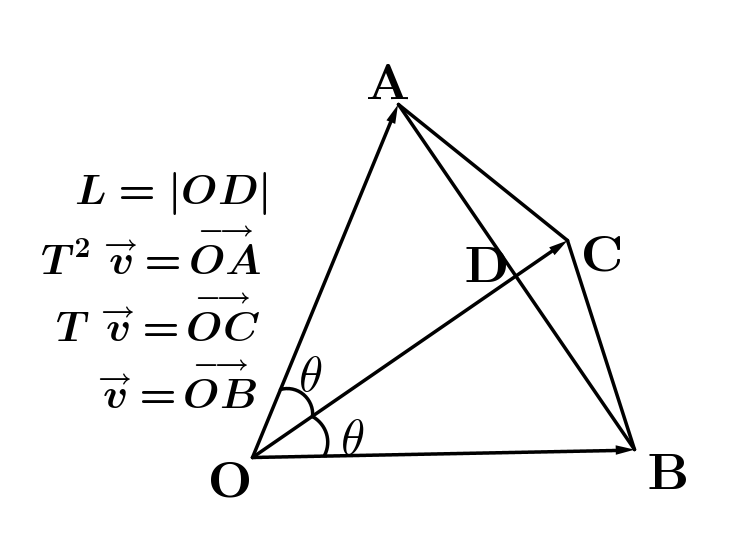
\includegraphics[width=4.4cm,height=3.2cm,scale=0.22]{diagram2.png}\par\vspace{-70pt}\quad
\hspace{180pt}{$\MathLeftMid{l}{Tv=\Frac{\left|\overset{\rightarrow}{v}\right|}{2L}\Par{T^2 v+v}\Rightarrow T=\Frac{\left|\overset{\rightarrow}{v}\right|}{2L}\Par{T^2+I}\\\vspace{8pt} L=\left|\overset{\rightarrow}{v}\right|\cos\theta\Rightarrow\Frac{\left|\overset{\rightarrow}{v}\right|}{2L}=\Frac{1}{2\cos\theta}}$}\par\quad
Hence $p\Par{T}=T^2-2\cos\theta\, T+I=0$ and $z^2-2\cos\theta\;z+1$ is the mini poly of $T.$\PfEnd\vspace{6pt}\quad
\Or Let $\Par{e_1,e_2}$ be the standard basis of $\Rbb^2.$ We use the pattern shown in [8.44].\par\quad
Because $Te_1=\cos\theta\;e_1+\sin\theta\;e_2,\;T^2e_1=\cos2\theta\;e_1+\sin2\theta\;e_2.$\par\vspace{2pt}\quad
Thus \;$ce_1+bTe_1=-T^2 e_1\Longleftrightarrow{}${\small$\begin{pmatrix}
	1 & \cos\theta\\
	0 & \sin\theta
\end{pmatrix}\begin{pmatrix}
	c \\ b
\end{pmatrix}$}${}={}${\small$\begin{pmatrix}
-\cos2\theta\\
-\sin2\theta
\end{pmatrix}$}. Now $\det=\sin\theta\neq 0,c=1,b=2\cos\theta.$\PfEnd\vspace{12pt}\quad
\Or $\Mt[\BigPar]{T,\Par{e_1,e_2}}={}${\small$\begin{pmatrix}\Blind{-}\cos\theta & \sin\theta\\-\sin\theta & \cos\theta
\end{pmatrix}$}. By (4E 5.B.11), the mini poly is $\Par{z\pm 1}$ or $\Par{z^2-2\cos\theta\,z+1}.$\PfEnd
\SepLine\pagebreak

\ProblemBnoor{\hypertarget{5BI4e11}{4E 5.B.11}}{
	\TextB{Suppose $V$ is a two-dim vecsp, $T\in\Lm{V}$, and the matrix of $T$}
	\TextB{with resp to some basis of \,$V$ is {\large$\begin{pmatrix} a & c\\ b & d\end{pmatrix}.$}}
	(a) \TextB{Show that $T^2 - \Par{a + d}T + \Par{ad - bc}I = 0.$}
	(b) \TextB{Show that the mini poly of $T$ equals}
	\TextB{\large\envFontDefault\centerline{$\MathLeftBrace{l}{z-a\qquad\qquad\qquad\qquad\qquad$ if $b=c=0$ and $a=d$,$\\ z^2-\Par{a+d}z+\Par{ad-bc}\quad$ \,\,otherwise.$}$}}
}\par\quad
(a) Suppose the basis is $\Par{v,w}$. Because $\MathLeftBrace{l}{Tv=av+bw\Rightarrow\Par{T-aI}v=bw,$ then apply $\Par{T-dI}$ to both sides. $\\ Tw=cv+dw\Rightarrow \Par{T-dI}w=cv,$ then apply $\Par{T-aI}$ to both sides. $}$\par\vspace{6pt}\quad\Ha
Hence $\Par{T-aI}\Par{T-dI}=bc I\Rightarrow T^2 - \Par{a + d}T + \Par{ad - bc}I = 0.$\par\quad
(b) If $b=c=0$ and $a=d.$ Then $\Mt{T}=${\small$\begin{pmatrix}a & 0\\ 0 & a\end{pmatrix}$}$=a\Mt{I}$. Thus $T=aI.$ Hence the mini poly is $z-a.$\par\quad\Hb
Otherwise, by (a), $z^2-\Par{a+d}z+\Par{ad-bc}$ is a poly multi of the mini poly.\par\quad\Hb
Now we prove that $T\not\in\Span{I},$ so that then the mini poly of $T$ has exactly degree $2.$\par\quad\Hb
( At least one of the assumption of (I),(II) below is true. )\par\quad\Hb
(I) Suppose $a=d,$ then $Tv=av+bw\not\in\Span{v},Tw=cv+aw\not\in\Span{w}.$\par\qquad
(II) Suppose at most one of $b,c$ is not $0.$ If $b=0,$ then $Tw\not\in\Span{w};$ If $c=0,$ then $Tv\not\in\Span{v}.$\PfEnd
\SepLine

\ProblemB{
	\TextB{Suppose $S,T\in\Lm{V},S$ is inv, and $p\in\PoF{}$. Prove that $Sp\Par{TS}=p\Par{ST}S.$}
}\par\quad
We prove $S\Par{TS}{^m}=\Par{ST}{^m} S$ for each $m\in\Nbb\,$ by induction.\par\quad
(i) If $m=0,1.$ Then $S\Par{TS}{^0}=I=\Par{ST}{^0}S;\;S\Par{TS}{^1}=\Par{ST}S.$\par\quad\Endi
(ii) If $m>1.$ Assume that $S\Par{TS}{^m}=\Par{ST}{^m} S.$\par\quad\Hii
Then $S\Par{TS}{^{m+1}}=S\Par{TS}{^m}\Par{TS}=\Par{ST}{^m} STS=\Par{ST}{^{m+1}}S.$\par\quad
Hence $\forall p\in\PoF{},Sp\Par{TS}=\sum_{k=1}^ma_kS\Par{TS}{^k}=\sum_{k=1}^ma_kp\Par{ST}{^k}S=\Sbra{\sum_{k=1}^ma_k\Par{TS}{^k}}S.$\PfEnd\vspace{2pt}
\Comment \,\,\,$p\Par{TS} = S^{-1} p\Par{ST}S,\;p\Par{ST} = Sp\Par{TS}S^{-1}.$\par
\Corollary \,\,\,\ProblemN[]{\hypertarget{5BI5}{5}}{
	Because $S$ is inv, $T\in\Lm{V}$ is arbitrary $\Longleftrightarrow R=ST$ is arbitrary.\TextN{}
	\Blind{\Corollary \,\,\,} Hence $\forall R\in\Lm{V},$ inv $S\in\Lm{V},p\Par{S^{-1}RS}=S^{-1}p\Par{R}S.$\TextN{\vspace{-4pt}}
}\SepLine

\ProblemBnoor{\hypertarget{5BI4e7}{4E 5.B.7}}{
	\TextB{Suppose $S, T\in\Lm{V}.$ Let $p,q$ be the mini polys of $ST,TS$ respectively.}
	(a) \TextB{If $V=\Fbb^2.$ Give an example such that $p\neq q;$ \;{\large\tgnr(b)} If $S$ or $T$ is inv. Prove that $p=q.$}
}\par\quad
(a) %Let $V=\Fbb^{\infty},$ $S\in\Lm{\Fbb^\infty}$ is the forward shift operator, $T\in\Lm{\Fbb^\infty}$ is the backward shift operator.\par\quad\Ha
%Then $ST(x_1,x_2,x_3,\dots)=(0,x_2,x_3,\dots)\Rightarrow 0,1$ are all the eigvals of $ST,$ $(ST)^2-(ST)=0.$\par\quad\Ha
%$TS(x_1,x_2,\dots)=(x_1,x_2,\dots)\Rightarrow 1$ is the only eigval of $TS,$ $TS=I.$\par\quad\Ha
Define $S$ by $S\Par{x,y}=\Par{x,x}.$ Define $T$ by $T\Par{x,y}=\Par{0,y}.$\par\quad\Ha
Then $ST\Par{x,y}=0,\,\,TS\Par{x,y}=\Par{0,x}$ for all $\Par{x,y}\in\Fbb^2.$ Thus $ST=0\neq TS$ and $\Par{TS}^2=0.$\par\quad\Ha
Hence the mini poly of $ST$ does not equal to the mini poly of $TS.$\par\quad
(b) Suppose $S$ is inv. Because $p,q$ are monic.\par\quad\Hb
$\MathRightBrace{l}{$
$p\Par{ST}=0=S p\Par{TS}S^{-1}\Rightarrow p\Par{TS}=0,p$ is a poly multi of $q\\ $
$q\Par{TS}=0=S^{-1} q\Par{ST}S\Rightarrow q\Par{ST}=0,q$ is a poly multi of $p$
$}\Rightarrow p=q.$\par\vspace{6pt}\quad\Hb
Reversing the roles of $S$ and $T$, we conclude that if $T$ is inv, then $p=q$ as well.\PfEnd
\SepLine

\ProblemN{\hypertarget{5BI11}{11}}{
	\TextNL{Suppose $\Fbb = \Cbb,$ $T\in\Lm{V}, p\in\PoC{}$, and $\alpha\in\Cbb.$}
	\TextNL{Prove that $\alpha$ is an eigval of $p\Par{T}$ $\Longleftrightarrow$ $\alpha = p\Par{\lambda}$ for some eigval $\lambda$ of $T$.}
}\par\quad
(a) Suppose $\alpha$ is an eigval of $p\Par{T}\Leftrightarrow \BigPar{p\Par{T}-\alpha I}$ is not inje.\par\quad\Ha
Write $p\Par{z}-\alpha=c\Par{z-\lambda_1}\cdots\Par{z-\lambda_m}\Rightarrow p\Par{T}-\alpha I=c\Par{T-\lambda_1 I}\cdots\Par{T-\lambda_m I}.$\par\quad\Ha
By \TIPS, $\exists\,\Par{T-\lambda_j I}$ not inje. Thus $p\Par{\lambda_j}-\alpha=0.$\par\quad
(b) Suppose $\alpha=p\Par{\lambda}$ and $\lambda$ is an eigval of $T$ with an eigvec $v.$ Then $p\Par{T}v=p\Par{\lambda}v=\alpha v.$\PfEnd\vspace{3pt}\quad\Hb
\Or Define $q$ by $q\Par{z}=p\Par{z}-\alpha.$ $\lambda$ is a zero of $q.$\par\quad\Hb
Because $q\Par{T}v=\BigPar{p\Par{T}-\alpha I}v=q\Par{\lambda}v=\BigPar{p\Par{\lambda}-\alpha}v=0.$\par\quad\Hb
Hence $q\Par{T}$ is not inje $\Rightarrow \BigPar{p\Par{T}-\alpha I}$ is not inje.\PfEnd
\SepLine

\ProblemNor{\hypertarget{5BI12}{12}}{4E.5.B.6}{
	\TextNL{Give an example of an operator on $\Rbb^2$}
	\TextNL{that shows the result above does not hold if $\Cbb$ is replaced with $\Rbb$.}
}\par\quad
Define $T\in\Lm{\Rbb^2}$ by $T\Par{w,z}=\Par{-z,w}.$\par\quad
By Problem (4E 5.B.11), $\Mt[\BigPar]{T,\Par{\Par{1,0},\Par{0,1}}}=\,${\small$\begin{pmatrix}0 & -1\\ 1 & 0\end{pmatrix}$}$\Rightarrow$ the mini poly of $T$ is $z^2+1.$\par\quad
Define $p$ by $p\Par{z}=z^2.$ Then $p\Par{T}=T^2=-I.$ Thus $p\Par{T}$ has eigval $-1.$\par\quad
While $\nexists\,\lambda\in\Rbb$ such that $-1=p\Par{\lambda}=\lambda^2.$\PfEnd
\SepLine

\ProblemBnoor{\hypertarget{5BI4e17}{4E 5.B.17}}{
	\TextB{Suppose $V$ is finite-dim, $T\in \Lm{V},\lambda\in\Fbb$, and $\,p\,$ is the mini poly of $T$.}
	\TextB{Show that the mini poly of $\Par{T - \lambda I}$ is the poly $q$ defined by $q\Par{z} = p\Par{z + \lambda}.$}
}\par\quad
$q\Par{T-\lambda I}=0\Rightarrow q$ is poly multi of the mini poly of $\Par{T-\lambda I}.$\par\quad
Suppose the degree of the mini poly of $\Par{T-\lambda I}$ is $n,$ and the degree of the mini poly of $T$ is $m.$\par\quad
%Write $q(z)=p(z+\lambda)=a_0+a_1(z+\lambda)+\dots+a_{m-1}(z+\lambda)^{m-1}+(z+\lambda)^m.$\par\quad
By definition of mini poly,\par\quad
$n$ is the smallest such that $\Par{T-\lambda I}^n\in\Span{I,\Par{T-\lambda I},\dots,\Par{T-\lambda I}^{n-1}};$\par\quad
$m$ is the smallest such that $T^m\in\Span{I,T,\dots,T^{m-1}}.$\par\quad
又 $T^k\in\Span{I,T,\dots,T^{k-1}}\Longleftrightarrow \Par{T-\lambda}^k\in\Span{I,\Par{T-\lambda I},\dots,\Par{T-\lambda I}^{k-1}}.$\par\quad
Thus $n=m.$ 又 $q$ is monic. By the uniqnes of mini poly.\PfEnd
\SepLine

\ProblemBnoor{\hypertarget{5BI4e18}{4E 5.B.18}}{
	\TextB{Suppose $V$ is finite-dim, $T\in \Lm{V},\lambda\in\Fbb\backslash\zeroSubs$, and $\,p\,$ is the mini poly of $T$.}
	\TextB{Show that the mini poly of $\lambda T$ is the poly q defined by $q\Par{z} = \lambda^{\deg p} p\Par{\frac{z}{\lambda}}$.}
}\par\quad
$q\Par{\lambda T}=\lambda^{\deg p}p\Par{T}=0\Rightarrow q$ is a poly multi of the mini poly of $\lambda T.$\par\quad
Suppose the degree of the mini poly of $\lambda T$ is $n,$ and the degree of the mini poly of $T$ is $m.$\par\quad
By definition of mini poly,\par\quad
$n$ is the smallest such that $\Par{\lambda T}^n\in\Span{\lambda I,\lambda T,\dots,\Par{\lambda T}^{n-1}};$\par\quad
$m$ is the smallest such that $T^m\in\Span{I,T,\dots,T^{m-1}}.$\par\quad
又 $\Par{\lambda T}^k\in\Span{\lambda I,\lambda T,\dots,\Par{\lambda T}^{k-1}}\Longleftrightarrow T^k\in\Span{I,T\dots,T^{k-1}}.$\par\quad
Thus $n=m.$ 又 $q$ is monic. By the uniqnes of mini poly.\PfEnd
\SepLine

\ProblemNor{\hypertarget{5BI18}{18}}{\hypertarget{5BI4e15}{4E 5.B.15}}{
	\TextNL{Suppose $V$ is a finite-dim complex vecsp with $\dim V > 0$ and $T\in\Lm{V}$.}
	\TextNL{Define $f:\Cbb\rightarrow\Rbb$ by $f\Par{\lambda} = \dim \range\Par{T-\lambda I}$.}
	\TextNL{Prove that $f$ is not a continuous function.}
}Note that $V$ is finite-dim.\par\quad
Let $\lambda_0$ be an eigval of $T.$ Then $\Par{T-\lambda_0 I}$ is not surj. Hence $\dim\range\Par{T-\lambda_0 I}<\dim V.$\par\quad
Because $T$ has finitely many eigvals. There exist a sequence of number $\Bra{\lambda_n}$ such that $\lim\limits_{n\rightarrow\infty}\lambda_n=\lambda_0$.\par\quad
And $\lambda_n$ is not an eigval of $T$ for each $n\Rightarrow\dim\range\Par{T-\lambda_n I}=\dim V\neq \dim\range\Par{T-\lambda_0 I}.$\par\quad
Thus $f\Par{\lambda_0}\neq \lim\limits_{n\rightarrow\infty}f\Par{\lambda_n}.$\PfEnd
\SepLine

\ProblemBnoor{\hypertarget{5BI4e9}{4E 5.B.9}}{
	\TextB{Suppose $T\in\Lm{V}$ is such that with resp to some basis of \,$V$,}
	\TextB{all entries of the matrix of $T$ are rational numbers.}
	\TextB{Explain why all coefficients of the mini poly of $T$ are rational numbers.}
}\par\quad
Let $\Par{v_1,\dots,v_n}$ denote the basis such that $\Mt[\BigPar]{T,\Par{v_1,\dots,v_n}}_{j,k}=A_{j,k}\in\Qbb$ for all $j,k=1,\dots,n$.\par\quad
Denote $\Mt[\BigPar]{v_j,\Par{v_1,\dots,v_n}}$ by $x_j$ for each $v_j.$\par\quad
Suppose $p$ is the mini poly of $T$ and $p\Par{z}=z^m+\dots+c_1 z+c_0.$ Now we show that each $c_j\in\Qbb.$\par\quad
Note that $\forall s\in\Nbp,\Mt{T^s}=\Mt{T}^s=A^s\in\Qbb^{n,n}$ and $T^s v_k=A^s_{1,k} v_1+\dots+A^s_{n,k}v_n$ for all $k\in\Bra{1,\dots,n}.$\par\vspace{6pt}\quad
Thus $\MathLeftBrace{l}{
\Mt{p\Par{T}v_1}=\Par{A^m+\dots+c_1 A+c_0 I}x_1=\sum\limits_{j=1}^n\Par{A^m+\dots+c_1 A+c_0 I}_{j,1}x_j=0;\\ \qquad\qquad\vdots \\
\Mt{p\Par{T}v_n}=\Par{A^m+\dots+c_1 A+c_0 I}x_n=\sum\limits_{j=1}^n\Par{A^m+\dots+c_1 A+c_0 I}_{j,n}x_j=0;
}$\par\quad
More clearly, $\MathLeftBrace{l}{
\Par{A^m+\dots+c_1 A+c_0 I}_{1,1}=\cdots=\Par{A^m+\dots+c_1 A+c_0 I}_{n,1}=0;\\\hspace{130pt}\vdots\hspace{8pt}\ddots\hspace{8pt}\vdots\\
\Par{A^m+\dots+c_1 A+c_0 I}_{1,n}=\cdots=\Par{A^m+\dots+c_1 A+c_0 I}_{n,n}=0;
}$\par\quad
Hence we get a system of $n^2$ linear equations in $m$ unknowns $c_0,c_1,\dots,c_{m-1}.$\par\quad
We conclude that $c_0,c_1,\dots,c_{m-1}\in\Qbb.$\PfEnd
\SepLine

\ProblemBnoor{\OR (\hypertarget{5BI4e16}{4E 5.B.16}), \OR (8.C.18)}[\Sbra]{
	\TextB{Suppose $a_0 ,\dots, a_{n-1}\in\Fbb.$ Let $T$ be the operator on $\Fbb^n$ such that\vspace{2pt}}
	\TextB{$\Mt{T}=\,${\normalsize$\begin{pmatrix}
	0 &   &        &  &   & -a_0     \\
	1 & 0 &        &  &   & -a_1     \\
	  & 1 & \ddots &  &   & \vdots   \\
	  &   & \ddots &  & 0 & -a_{n-2} \\
	0 &   &        &  & 1 & -a_{n-1}
\end{pmatrix} $}, with resp to the standard basis $\Par{e_1,\dots,e_n}$.\vspace{4pt}}
	\TextB{Show that the mini poly of $T$ is $\,p\,$ defined by $p\Par{z}=a_0 + a_1 z + \dots + a_{n-1} z^{n-1} + z^n$.}
	\vspace{-2pt}\TextB{\small $\Mt{T}$ is called the {\tgsc companion matrix} of the poly above. This exercise shows that every monic poly is the mini poly of some operator.}
	\vspace{-2pt}\TextB{\small Hence a formula or an algorithm that could produce exact eigvals for each operator on each $\Fbb^n$ could then produce exact zeros for}
	\vspace{-2pt}\TextB{\small each poly  $[$ by 8.36(b) $]$. Thus there is no such formula or algorithm. However, efficient numeric methods exist for obtaining very good}
	\TextB{\small approximations for the eigvals of an operator.}
}Note that $\Par{e_1,Te_1,\dots,T^{n-1}e_1}$ is linely inde. 又 The deg of mini poly is at most $n.$\par\quad
$T^n e_1=\cdots=T^{n-k}e_{1+k}=\cdots=T e_n=-a_0 e_1-a_1 e_2-a_2 e_3-\dots-a_{n-1}e_n$\par
$=\Par{-a_0 I-a_1 T-a_2 T^2-\dots-a_{n-1}T^{n-1}}e_1.$ Thus $p\Par{T}e_1=0=p\Par{T}e_j$ for each $e_j=T^{j-1}e_1.$\PfEnd
\SepLine

\BulletPointX{\Large\textsc{Eigenvalues On Odd-Dimensional Real Vector Spaces}}\par
\ProblemB{
	\textsc{Even-Dimensional Null Space}\TextB{}
	\TextB{Suppose $\Fbb=\Rbb,$ $V$ is finite-dim, $T\in\Lm{V}$ and $b, c\in\Rbb$ with $b^2 < 4c$.}
	\TextB{Prove that $\dim\null\Par{T^2 + bT + cI}$ is an even number.}
}\par\quad
Denote $\null\Par{T^2 + bT + cI}$ by $R.$ Then $T\mmid_R+bT\mmid_R+cI_R=\Par{T+bT+cI}\mmid_R=0\in\Lm{R}.$\par\quad
Suppose $\lambda$ is an eigval of $T_R$ with an eigvec $v\in R.$\par\quad
Then $0=\Par{T\mmid_R^2+bT\mmid_R+cI_R}\Par{v}=\Par{\lambda^2+\lambda b+c}v=\BigPar{\Par{\lambda+b}^2+c-\Frac{b^2}{4}}v.$\par\quad
Because $c-\Frac{b^2}{4}>0$ and we have $v=0.$ Thus $T_R$ has no eigvals.\par\quad
Let $U$ be an invar subsp of $R$ that has the largest, even dim among all invar subsps.\par\quad
Assume that $U\neq R.$ Then $\exists\,w\in R$ but $w\not\in U.$ Let $W$ be such that $\Par{w,T\mmid_R w}$ is a basis of $W.$\par\quad
Because $T\mmid_R^2 w=-bT\mmid_R w-cw\in W.$ Hence $W$ is an invar subsp of dim $2.$\par\quad
Thus $\dim \Par{U+W}=\dim U+2-\Dim\Par{U\cap W},$ where $U\cap W=\zeroSubs,$\par\qquad\qquad
for if not, because $w\not\in U,T\mmid_R w\in U,$\par\qquad\qquad $U\cap W$ is invar under $T\mmid_R$ of one dim ( impossible because $T\mmid_R$ has no eigvecs ).\par\quad
Hence $U+W$ is even-dim invar subsp under $T\mmid_R$, contradicting the maximality of $\dim U.$\par\quad
Thus the assumption was incorrect. Hence $R=\null\Par{T^2+bT+cI}=U$ has even dim.\PfEnd
\SepLine

\ProblemB{
	\textsc{Operators On Odd-Dimensional Vector Spaces Have Eigenvalues}\TextB{}
	(a) \TextB{Suppose $\Fbb=\Cbb.$ \tgnr\large Then by [5.21], we are done.}
	(b) \TextB{Suppose $\Fbb=\Rbb,$ $V$ is finite-dim, and $\dim V=n$ is an odd number.}
	\Hb\TextB{Let $T\in\Lm{V}$ and the mini poly is $\,p\,$. Prove that $T$ has an eigval.}
}\par\quad
(i) If $n=1,$ then we are done.\par\quad\Endi
(ii) Suppose $n\geqslant 3.$ Assume that every operator, on odd-dim vecsps of dim less than $n,$ has an eigval.\par\quad\Hii
If $p$ is a poly multi of $\Par{x - \lambda}$ for some $\lambda\in\Rbb,$ then by [8.49] $\lambda$ is an eigval of $T$ and we are done.\par\quad\Hii
Now suppose $b, c\in\Rbb$ such that $b^2 < 4c$ and $p$ is a poly multi of $x^2 + bx + c$ (see [4.17]).\par\quad\Hii
Then $\exists\,q\in\PoR{}$ such that $p\Par{x} = q\Par{x}\Par{x^2 + bx + c}$ for all $x\in\Rbb.$\par\quad\Hii
Now $0 = p\Par{T} = \BigPar{q\Par{T}}\Par{T^2 + bT + cI},$ which means that $q\Par{T}\mmid_{\range\Par{T^2+bT+cI}}=0.$\par\quad\Hii
Because $\deg q < \deg p$ and $p$ is the mini poly of $T$, hence $\range\Par{T^2 + bT + cI}\neq V$.\par\quad\Hii
又 $\dim V$ is odd and $\dim\null\Par{T^2 +bT+cI}$ is even ( by our previous result ).\par\quad\Hii
Thus $\dim V - \dim \null\Par{T^2 + bT + cI}=\dim \range\Par{T^2 + bT + cI}$ is odd.\par\quad\Hii
By [5.18], $\range\Par{T^2 + bT + cI}$ is an invar subsp of $V$ under $T$ that has odd dim less than $n.$\par\quad\Hii
Our induction hypothesis now implies that $T\mmid_{\range\Par{T^2 + bT + cI}}$ has an eigval.\par\quad
By mathematical induction.\PfEnd
\SepLine

\ProblemBnoor{\hypertarget{5BI2e24}{2E Ch5.24}}{
	\TextB{Suppose $\Fbb=\Rbb,T\in\Lm{V}$ has no eigvals.} \TextB{Prove that every invar subsp of \,$V$ under $T$ is even-dim.}
}\par\quad
Suppose $U$ is such a subsp. Then $T\mmid_U\in\Lm{U}.$
We prove by contradiction.\par\quad
If $\dim U$ is odd, then $T\mmid_U$ has an eigval and so is $T,$ so that $\exists$ invar subsp of $1$ dim, contradicts.\PfEnd
\SepLine

\ProblemBnoor{\hypertarget{5BI4e29}{4E 5.B.29}}{
	\TextB{Show that every operator on a finite-dim vecsp of dim $\geq 2$ has a $2$-dim invar subsp.}
}\par\quad
Using induction on $\dim V.$\par\quad
(i) $\dim V=2,$ we are done.\par\quad\Endi
(ii) $\dim V>2.$ Assume that the desired result is true for vecsp of smaller dim.\par\quad\Hii
Suppose $p$ is the mini poly of degree $m$ and $p\Par{z}=\Par{z-\lambda_1}\cdots\Par{z-\lambda_m}.$\par\quad\Hii
If $\,T=\lambda I\,\Par{\,\Leftrightarrow m=1\,\vee\,m=-\infty\,},$ then we are done. ( $m\neq 0$ because $\dim V\neq 0.$ )\par\quad\Hii
Now define a $q$ by $q\Par{z}=\Par{z-\lambda_1}\Par{z-\lambda_2}$.\par\quad\Hii
By assumption, $T\mmid_{\null q\Par{T}}$ has an invar subsp of dim $2.$\PfEnd
\SepLine

\ChEnd

% 6h
\ChDecl{Ch5BII}{5.B: II}{}\orMode{\hLk{5BII9}{9}\;\;\hLk{5BII14}{14}\;\;\hLk{5BII15}{15}\;\;\hLk{5BII20}{20}\;\;|\;\;\hLk{5BII4e1}{4E: 1,}\;\;\hLk{5BII4e2}{2,}\;\;\hLk{5BII4e3}{3,}\;\;\hLk{5BII4e4}{4,}\;\;\hLk{5BII4e5}{5,}\;\;\hLk{5BII4e6}{6,}\;\;\hLk{5BII4e7}{7,}\;\;\hLk{5BII4e8}{8,}\;\;\hLk{5BII4e9}{9,}\;\;\hLk{5BII4e10}{10}\;\;\hLk{5BII4e11}{11,}\;\;\hLk{5BII4e12}{12,}\;\;\hLk{5BII4e13}{13,}\;\;\hLk{5BII4e14}{14}}{[1]: ; [2]: ; [3]: .}

\ProblemBnoor{\hypertarget{5BII4e1}{4E 5.C.1}}{
	\TextB{Prove or give a counterexample\hspace{1pt}$:$}
	\TextB{If $T\in \Lm{V}$ and $T^2$ has an upper-trig matrix, then $T$ has an upper-trig matrix.}
}\par
\SepLine

\ProblemBnoor{\hypertarget{5BII4e2}{4E 5.C.2}}{
	\TextB{Suppose $A$ and $B$ are upper-trig matrices of the same size,}
	\TextB{with $\alpha_1 , \dots , \alpha_n$ on the diag of $A$ and $\beta_1 , \dots , \beta_n$ on the diag of $B$.}
	(a) \TextB{Show that $A + B$ is an upper-trig matrix with $\alpha_1 + \beta_1 , \dots , \alpha_n + \beta_n$ on the diag.}
	(b) \TextB{Show that $AB$ is an upper-trig matrix with $\alpha_1 \beta_1 , \dots , \alpha_n \beta_n$ on the diag.}
}\par
\SepLine

\ProblemBnoor{\hypertarget{5BII4e3}{4E 5.C.3}}{
	\TextB{}
	\TextB{Suppose $T\in \Lm{V}$ is inv and $B=\Par{v_1 , \dots , v_n}$ is a basis of \,$V$ such that}
	\TextB{$\Mt{T,B}=A$ is upper trig, with $\lambda_1 , \dots , \lambda_n$ on the diag.}
	\TextB{Show that the matrix of $\Mt{T^{-1},B}=A^{-1}$ is also upper trig, with
{\normalsize$\Frac{1}{\lambda_1},\dots,\Frac{1}{\lambda_n}$} on the diag.}
}\par
\SepLine

\ProblemNnoor{\hypertarget{5BII9}{9}}{\hypertarget{5BII4e7}{4E 5.C.7}}{
	\TextN{Suppose $V$ is finite-dim, $T\in \Lm{V}$, and $v \in V$.}
	(a) \TextN{Prove that $\exists\,!$ monic poly $p_v$ of smallest degree such that $p_v \Par{T}v = 0$.}
	(b) \TextN{Prove that the mini poly of $T$ is a poly multi of $p_v$.}
}
\SepLine


\ProblemNor{\hypertarget{5BII14}{14}}{\hypertarget{5BII4e4}{4E 5.C.4}}{
	\TextNL{ Give an operator $T$ such that with resp to some basis,}
	\TextNL{$\Mt{T}_{k,k}=0$ for each $k$, while $T$ is inv.}
}
\par
\SepLine

\ProblemNor{\hypertarget{5BII15}{15}}{\hypertarget{5BII4e5}{4E 5.C.5}}{
	\TextNL{Give an operator $T$ such that with resp to some basis,}
	\TextNL{$\Mt{T}_{k,k}\neq 0$ for each $k$, while $T$ is not inv.}
}\par


\par
\SepLine

\ProblemNor{\hypertarget{5BII20}{20}}{\normalsize \OR \hypertarget{5BII4e6}{4E 5.C.6}}{
	\TextNL{}
	\TextNL{Suppose $\Fbb=\Cbb,$ $V$ is finite-dim, and $T\in\Lm{V}$.}
	\TextNL{Prove that if $k\in\Bra{1,\dots,\dim V},$ then \,$V$ has a $k$ dim subsp invar under $T$.}
}\par
\SepLine

\ProblemBnoor{\hypertarget{5BII4e8}{4E 5.C.8}}{
	\TextB{Suppose $V$ is finite-dim, $T\in \Lm{V}$, and $\exists\,v \in V\backslash\zeroSubs$ such that $T^2 v + 2Tv = -2v$.}
	(a) \TextB{Prove that if $\Fbb=\Rbb,$ then $\nexists$ a basis of \,$V$ with resp to which $T$ has an upper-trig matrix.}
	(b) \TextB{Prove that if $\Fbb=\Cbb$ and $A$ is an upper-trig matrix that equals the matrix of $T$}
	\Hb\TextB{with resp to some basis of \,$V$, then $-1 + \i$ or $-1 - \i$ appears on the diag of $A$.}
}\par
\SepLine

\ProblemBnoor{\hypertarget{5BII4e9}{4E 5.C.9}}{
	\TextB{Suppose $B\in\Fbb^{n,n}$ with complex entries.}
	\TextB{Prove that $\exists$ inv $A\in\Fbb^{n,n}$ with complex entries such that $A^{-1} BA$ is an upper-trig matrix.}
}\par

\par
\SepLine

\ProblemBnoor{\hypertarget{5BII4e10}{4E 5.C.10}}{
	\TextB{Suppose $T\in \Lm{V}$ and $\Par{v_1,\dots,v_n}$ is a basis of \,$V$.}
	\TextB{Show that the following are equi.}
	(a) \TextB{The matrix of $T$ with resp to $\Par{v_1,\dots,v_n}$ is lower trig.}
	(b) \TextB{$\Span{v_k,\dots,v_n}$ is invar under $T$ for each $k=1,\dots,n$.}
	(c) \TextB{$Tv_k\in\Span{v_k,\dots,v_n}$ for each $k=1,\dots,n$.}
}\par
\SepLine

\ProblemBnoor{\hypertarget{5BII4e11}{4E 5.C.11}}{
	\TextB{Suppose $\Fbb=\Cbb$ and $V$ is finite-dim.}
	\TextB{Prove that if $T\in \Lm{V}$, then $T$ has a lower-trig matrix with resp to some basis.}
}\par
\SepLine

\ProblemBnoor{\hypertarget{5BII4e12}{4E 5.C.12}}{
	\TextB{}
	\TextB{Suppose $V$ is finite-dim, $T\in \Lm{V}$ has an upper-trig matrix with resp to some basis,}
	\TextB{and $U$ is a subsp of \,$V$ that is invar under $T$.}
	(a) \TextB{Prove that $T\mmid_U$ has an upper-trig matrix with resp to some basis of $U$.}
	(b) \TextB{Prove that $T\mySlash U$ has an upper-trig matrix with resp to some basis of \,$V\mySlash U$.}
}\par


\par
\SepLine

\ProblemBnoor{\hypertarget{5BII4e13}{4E 5.C.13}}{
	\TextB{Suppose $V$ is finite-dim, $T\in \Lm{V}$. Suppose $U$ is an invar subsp of \,$V$ under $T$}
	\TextB{such that $T\mmid_U$ has an upper-trig matrix and also $T\mySlash U$ has an upper-trig matrix.}
	\TextB{Prove that $T$ has an upper-trig matrix.}
}\par


\par
\SepLine

\ProblemBnoor{\hypertarget{5BII4e14}{4E 5.C.14}}{
	\TextB{Suppose $V$ is finite-dim and $T\in \Lm{V}$.}
	\TextB{Prove that $T$ has an upper-trig matrix $\Longleftrightarrow$ $T\apostrophe$ has an upper-trig matrix.}
}\par


\par
\SepLine

\ChEnd

\ChDecl{Ch5C}{5.C} % 10h

XXXX


\par
\SepLine

\ChEnd
\ChDecl{Ch5E}{5.E* (4E)}{}\orMode{\hLk{5E1}{1}\;\;\hLk{5E2}{2}\;\;\hLk{5E3}{3}\;\;\hLk{5E4}{4}\;\;\hLk{5E5}{5}\;\;\hLk{5E6}{6}\;\;\hLk{5E7}{7}\;\;\hLk{5E8}{8}\;\;\hLk{5E9}{9}\;\;\hLk{5E10}{10}}{}
% 0.5h/4h

\ProblemN{1}{
	\TextN{Give an example of two commuting operators $S, T\in\Fbb^4$ such that}
	\TextN{there is an invar subsp of $\Fbb^4$ under $S$ but not under $T$}
	\TextN{and an invar subsp of $\Fbb^4$ under $T$ but not under $S$.}
}
\par
\SepLine

\ProblemN{2}{
	\TextN{Suppose $\mathcal{E}$ is a subset of $\Lm{V}$ and every element of $\mathcal{E}$ is diagable.}
	\TextN{Prove that $\exists$ a basis of \,$V$ with resp to which}
	\TextN{every element of $\mathcal{E}$ has a diag matrix $\Longleftrightarrow$ every pair of elements of $\mathcal{E}$ commutes.}
	\TextN{{\normalsize This exercise extends [5.76], which considers the case in which $\mathcal{E}$ contains only two elements.}}\hspace{0.5pt}
	\TextN{{\normalsize For this exercise, $\mathcal{E}$ may contain any number of elements, and $\mathcal{E}$ may even be an infinite set.}}
}\par
\SepLine

\ProblemN{3}{
	\TextN{Suppose $S, T\in\Lm{V}$ are such that $ST = TS$. Suppose $p\in\PoF{}$.}
	(a) \TextN{Prove that $\null p\Par{S}$ is invar under $T$.}
	(b) \TextN{Prove that $\range p\Par{S}$ is invar under $T$.}
	\TextN{See \NOTEFOR [5.17] for the special case $S = T$.}
}\par
\SepLine

\ProblemN{4}{
	\TextN{Prove or give a counterexample\hspace{1pt}$:$}
	\TextN{A diag matrix $A$ and an upper-trig matrix $B$ of the same size commute.}
}\par
\SepLine

\ProblemN{5}{
	\TextN{Prove that a pair of operators on a finite-dim vecsp commute $\Longleftrightarrow$ their dual operators commute.}
}\par
\SepLine

\ProblemN{6}{
	\TextN{Suppose $V$ is a finite-dim complex vecsp and $S, T\in\Lm{V}$ commute.}
	\TextN{Prove that $\exists\,\alpha,\lambda\in\Cbb$ such that $\range\Par{S -\alpha I} + \range\Par{T -\lambda I}\neq V$.}
}\par
\SepLine

\ProblemN{7}{
	\TextN{Suppose $V$ is a complex vecsp, $S\in\Lm{V}$ is diagable, and $T$ commutes with $S$.}
	\TextN{Prove that $\exists$ basis $B$ of $V$ such that $S$ has a diag matrix with resp to $B$}
	\TextN{and T has an upper-trig matrix with resp to $B$.}
}\par
\SepLine

\ProblemN{8}{
	\TextN{Suppose $m = 3$ in Example [5.72]}
	\TextN{and $D_x , D_y$ are the commuting partial differentiation operators on $\Po_3\Par{\Rbb^2}$ from that example.}
	\TextN{Find a basis of $\Po_3\Par{\Rbb^2}$ with resp to which $D_x$ and $D_y$ each have an upper-trig matrix.}
}\par
\SepLine

\ProblemN{9}{
	\TextN{Suppose $V$ is a finite-dim nonzero complex vecsp.}
	\TextN{Suppose that $\mathcal{E}\subseteq\Lm{V}$ is such that $S$ and $T$ commute for all $S, T\in\mathcal{E}$.}
	(a) \TextN{Prove that $\exists\,v\in V$ is an eigvec for every element of $\mathcal{E}$.}
	(b) \TextN{Prove that $\exists$ a basis of \,$V$ with resp to which every element of $\mathcal{E}$ has an upper-trig matrix.}
}\par
\SepLine

\ProblemN{10}{
	\TextNL{Give an example of two commuting operators $S, T$ on a finite-dim real vecsp such that}
	\TextNL{$S + T$ has a eigval that does not equal an eigval of $S$ plus an eigval of $T$}
	\TextNL{and $ST$ has a eigval that does not equal an eigval of $S$ times an eigval of $T$.}
}
\par
\SepLine
\ChEnd

